\documentclass[11pt,a4paper]{article}

\usepackage[a4paper,margin=0.9in,footskip=0.20in]{geometry}

% those are the packages loaded
\usepackage[T1]{fontenc}
\usepackage[utf8]{inputenc}
\usepackage{authblk}
%\usepackage{hyperref}
\usepackage[xindy]{glossaries}
\usepackage{graphicx}
\usepackage{mathtools}
\usepackage{courier}
\usepackage[titletoc,toc,title]{appendix}
\usepackage{lineno}
\usepackage{tipa}
\usepackage{dirtytalk}
\usepackage{array}
\usepackage{makecell}
\usepackage{longtable, tabu}

\usepackage{xargs} 
\usepackage[pdftex,dvipsnames]{xcolor}
\usepackage[colorinlistoftodos,prependcaption,textsize=tiny]{todonotes}
\newcommandx{\unsure}[2][1=]{\todo[linecolor=red,backgroundcolor=red!25,bordercolor=red,#1]{#2}}
\newcommandx{\change}[2][1=]{\todo[linecolor=blue,backgroundcolor=blue!25,bordercolor=blue,#1]{#2}}
\newcommandx{\info}[2][1=]{\todo[linecolor=OliveGreen,backgroundcolor=OliveGreen!25,bordercolor=OliveGreen,#1]{#2}}
\newcommandx{\improvement}[2][1=]{\todo[linecolor=Plum,backgroundcolor=Plum!25,bordercolor=Plum,#1]{#2}}
\newcommandx{\thiswillnotshow}[2][1=]{\todo[disable,#1]{#2}}

%\usepackage{algorithm}
%%\usepackage{algpseudocode}
%\usepackage{algorithmic}

\usepackage{algorithm}
\usepackage{caption}
\usepackage{algorithmic}
%\usepackage{algpseudocode}

\newcommand{\norm}[1]{\left\lVert#1\right\rVert}
\newcommand{\CC}{C\nolinebreak\hspace{-.05em}\raisebox{.4ex}{\tiny\bf +}\nolinebreak\hspace{-.10em}\raisebox{.4ex}{\tiny\bf +}}
\renewcommand\theadalign{cb}
\renewcommand\theadfont{\bfseries}
\renewcommand\theadgape{\Gape[4pt]}
\renewcommand\cellgape{\Gape[4pt]}
%\renewcommand{\abstractname}{Executive Summary}

% silvio
\usepackage{color}
\definecolor{Red}{rgb}{1.0,0.0,0.0}
\newcommand\silvio[1]{\textcolor{Red}{(Silvio: #1)}}

% url cites
\usepackage{url}

% Use nameref to cite supporting information files (see Supporting Information section for more info)
\usepackage{nameref,hyperref}

% this is for the title
\title{Towards a Massively Scaling \gls{cpu} Implementation of Cortical Dynamics, a Phonetic Invariance Case Study Explanation}

% those are the authors
\author[1]{Dario Dematties \thanks{Corresponding author \\ E-mail: ddematties@fi.uba.ar}}
\author[2]{George K. Thiruvathukal}
\author[3]{Silvio Rizzi}
\author[5]{Alejandro Wainselboim}
\author[1,4]{B. Silvano Zanutto}

%those are the authors' affiliations
\affil[1]{Instituto de Ingeniería Biomédica, Facultad de Ingeniería, Universidad de Buenos Aires,
Ciudad Autonoma de Buenos Aires, Argentina}
\affil[2]{Computer Science Department, Loyola University Chicago, Chicago, Illinois, United States}
\affil[3]{Argonne National Laboratory, Lemont, Illinois, United States}
\affil[4]{Instituto de Biología y Medicina Experimental-CONICET,
Ciudad Autonoma de Buenos Aires, Argentina}
\affil[5]{Instituto de Ciencias Humanas, Sociales y Ambientales, Centro Cient\'ifico Tecnol\'ogico-CONICET,
Ciudad de Mendoza, Mendoza, Argentina}

% this command generates the glossary:
\makeglossaries

\loadglsentries{acronyms.tex}

% here is where the document starts
\begin{document}

\linenumbers

%\glsaddall

% the title is inserted here
\maketitle

%this is a kind of abstract called executive summary
\begin{abstract}

\end{abstract}



















% this is the first section in my paper; it is called "Introduction"
\section{Introduction}

%\subsection{Motivation}

%Behavioral evidence shows that humans and other animals can classify phonemes as well as other linguistic units categorically. They can also generalize in the presence of the variability imposed by different speakers with different pitches and prosody, even in noisy and reverberant environments~\cite{kuhl_1975, kuhl_1983, kluender_1998, pons_2006, hienz_1996, dent_1997, lotto_1997}.

%Neurophysiological evidence support such behavior revealing the existence of spectro-temporal tuning in naive ferrets' \gls{a1}. Cortical activations measured in such animals support phonetic discrimination~\cite{mesgarani_2008}, even when stimuli is distorted by additive noise and reverberation \cite{mesgarani_2014A}.

%Which are the neuroanatomical and neurophysiological features in cortical tissue that support such evidence? Although many computational theories have been developed, they only explain relevant aspects of phonetic acquisition~\cite{rasanen_2012}. Others are mainly proposed to improve audio classification accuracy using \glspl{cdbn} \cite{Lee:2009:UFL:2984093.2984217} and \glspl{dmn}~\cite{silos_2016}. Such approaches neglect important biological properties recently found in cortical tissue.

%Instead, we implemented a computational theory which incorporates specific properties present in the mammalian cortex. We foresee such properties as relevant for the acquisition of the sequential phonotactic rules of a language. 

%\subsection{Neuroanatomical and neurophysiological features in mammalian cortical tissue}

%\begin{itemize}

%\item First, cortical cells are aligned into restricted domains for common receptive field locations called \glspl{cc}~\cite{mountcastle_1955, mountcastle_1957, hubel_1962, hubel_1968}. \glspl{cc} are internally composed by cortical mini-columns. Cortical mini-columns are clusters of cells which respond to stimuli with similar characteristics (Fig. \ref{fig:Biological}).

%\begin{figure}[h!]
    %\centering
    %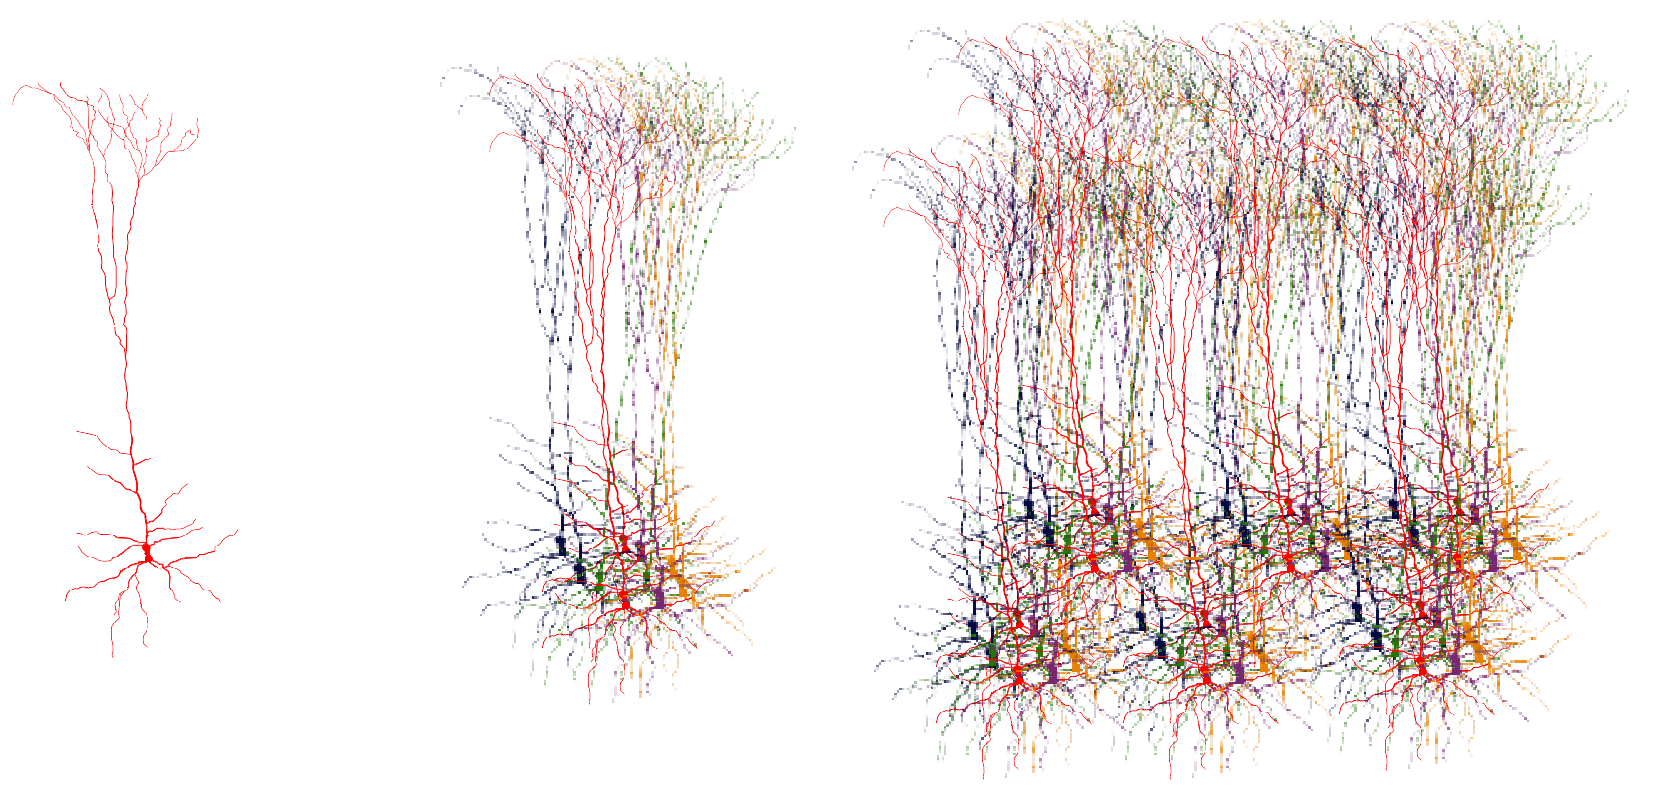
\includegraphics[width=0.6\textwidth]{Biological.png}
    %\caption{Cortical tissue organization. Left: Pyramidal cell. The most common excitatory neuron in cortical tissue.
    %Center: Cortical mini-column. A cluster on neural cells which responds to stimuli of similar characteristics.
    %Right: Cortical Column. A group of mini-columns with a common receptive field location.
    %Adapted from (Fabuio, Own work, CC BY 4.0, \url{https://commons.wikimedia.org/w/index.php?curid=60707501)}}
    %\label{fig:Biological}
%\end{figure}


%\item Second, cortical adaptation to contextual stimuli \cite{KRAUSE201436,doi:10.1167/16.13.1} is thought to enhance efficiency in the codification of sensory information. In this manner, a reduction in the responses to frequent sounds by means of inhibitory networks, may enhance cortical sensitivity to rare sounds that may represent unexpected events~\cite{Natan2015ComplementaryCO,nachum_2003,Javitt11962}.

%\item Third, the mammalian cortex processes information by means of \glspl{sdr}~\cite{barth_2012}. This mechanism, found in mice and humans, allows robust and low-error-rate discrimination of stimuli representations minimizing the neuronal activation required during the task in relation to the neural resources available for the representation~\cite{ahmad_2016}.

%\item Finally, in Hawkins et al. \cite{hawkins_2016} it is hypothetized that \glspl{sdr} arise from partial and extended depolarization of cells soma as the result of independent dendritic \gls{nmda} branch activations. In this mechanism, dendrites behave like independent learning elements becoming active by the excitation of certain number of distal synapses~\cite{antic_2010, major_2013}.

%\end{itemize}




\subsection{Our Contributions}

%\begin{itemize}

%\item We implemented a completely unsupervised and biologically inspired computational model which incorporates the above mentioned cortical features. Our model returns phonetic classification accuracy levels similar to those of state-of-the-art deep pattern classification approaches.

%\item We implemented our algorithms in standard \CC14 using \gls{stl} containers and the \gls{oop} paradigm in a set of classes interrelated by inheritance and composition.
%\item We parallelized the code by means of a hybrid \gls{mpi}+\gls{omp} paradigm and used \gls{mpi} I/O parallel file system.
%\item We implemented our own set of libraries in order to save the model status in Matlab/Octave file formats.
%\item Our implementation has Checkpoint and Restart capacity in its training stage where there is total flexibility in terms of the number of ranks with which the execution is restarted.
%\item In order to produce the inputs from auditory streams we followed main guidelines from Chi T. et al.~\cite{chi_2005}. To that end, we implemented an algorithm called \gls{mrstsa}. Our implementation follows primarily the cortical section in~\cite{chi_2005} rather than its sub-cortical counterpart. We implemented the algorithm in C and parallelized it by means of \gls{mpi}-\gls{omp} hybrid paradigm using \gls{omp} parallel sections.
%\item In order to generate the corpora audio files we call a Festival text to speech synthesizer~\cite{festival2014} implementing a Python code parallelized by means of \gls{mpi} package for Python called mpi4py.
%\item We performed all computational experiments on Cooley, a visualization and analysis cluster at Argonne National Laboratory.

	%\begin{itemize}
		%\item We ran science simulations using up to 49 nodes (one \gls{mpi} rank per node) and 9 \gls{omp} threads per node/rank. We tested the phonetic feature invariance capacity of our cortical implementation--in a stage called \gls{el}--in several word classification tasks.
		%\item We ran science tests on several models with different sizes and implemented a procedure similar to \emph{Self-taught Learning} developed in \cite{Raina:2007:SLT:1273496.1273592}. 
		%\item We compared the \gls{el} performance with the performance of the features returned by the \gls{mrstsa} algorithm by means of \gls{svm} classification of the features delivered by each algorithm (Fig. \ref{fig:Experiment}).
		%\item We ran performance tests on the \gls{el} using up to 64 nodes (one \gls{mpi} rank per node) and 12 \gls{omp} threads per node/rank. We performed strong and weak scaling tests on Cooley nodes.
		%\item We ran performance tests on audio corpora generation algorithm in python using up to 6 nodes running 64 \gls{mpi} processes on 64 \glspl{cpu}. We performed strong and weak scaling tests on Cooley nodes.
		%\item We ran performance tests on the \gls{mrstsa} algorithm using up to 64 nodes (one \gls{mpi} rank per node) and up to 5 \gls{omp} threads per node/rank. We performed strong and weak scaling tests on Cooley nodes.

	%\end{itemize}

%\end{itemize}





\section{Literature Review}

%To understand how phonetic categories and word-like units are acquired, several computational theories have been developed \cite{rasanen_2012}. In the context of such theories, the main idea has been to explain relevant aspects of phonetic acquisition by means of human engineered features. Nevertheless, \emph{lack of invariance} phenomenon in speech perception \cite{appelbaum_1996} seems to be one of those scientific problems which cannot be solved by spontaneous human reasoning, given the immense amount of interrelated variables involved in phonetic categorization processes. In that sense, \emph{deep learning} architectures--as a subfield inside of \emph{representation learning}--have shown unprecedented performance in the assistance of conventional machine learning techniques, which for decades  required careful engineering in order to reach an effective feature extraction design \cite{lecun_2015}.


\subsection{\glspl{cpu} vs. \glspl{gpu} for \gls{ai} applications}

\glspl{cpu} pipeline their instructions to the extreme in order to keep all the datapath in the chip busy. Superscalar designs in \glspl{cpu} allow each processor to actually have multiple datapaths, in this way multiple instructions can be exectuted simultaneously, one in each datapath. It is not uncommon for a superscalar \gls{cpu} to have multiple \glspl{alu} and \glspl{fpu}, for each datapath. Vector processors, or \gls{simd} processors--which are a more specific variant of superscalar architectures--have specialized hardware for performing vector operations such as vector addition, vector multiplication, and other operations. Vector processors perform an instruction on all data elements of a vector or  array simultaneously--in parallel. In a superscalar or similar processor design, there are multiple execution units that can be used to process pieces of data simultaneously. However, these execution units are not always used at the same time, and some processing power is lost. It is possible to feed instructions to all the execution units by taking the instructions out of their original order. \gls{oooe} is a mechanism that a processor has for executing instructions out of their original order, in an attempt to do more work in parallel and execute programs faster. Hyperthreading is the name for a technology developed by Intel which works by duplicating some architectural components of the processor, such as the status flags, the control registers, and the general purpose registers. Hyperthreading does not, however, duplicate any of the execution units. In a hyperthreaded system, it appears to the operating system that there are two or more separate processors, when there is only one processor. The \gls{oooe} engine feeds instructions from multiple separate execution threads to the execution cores, in an atempt to keep all of the cores simultaneously busy. In general hyperthreading increases performance, although in some cases this additional complexity could actually ending up decreasing it. Taking the idea of superscalar operations to the next level, companies put multiple microprocessor cores onto a single chip and make the cores run in parallel.

Modern \glspl{gpu} are highly parallel programmable processors which reach peak arithmetic and memory bandwidth that could substantially outpace its \gls{cpu} counterparts for some specific tasks. Programmable units in a \gls{gpu} follow a \gls{spmd} programming model. For efficiency, the \gls{gpu} processes many elements (vertices or fragments in an image for example) in parallel using the same program. Each element is independent from the other elements, and in the base programming model, elements cannot communicate with each other. All \gls{gpu} programs must be structured in this way: many parallel elements, each processed in parallel by a single program. A code written in this manner is considered \gls{simd}.

\glspl{gpgpu} is a methodology for \gls{hpc} that uses graphics processing units to process data. The characteristics of graphics algorithms that have enabled the development of extremely high-performance special purpose graphics processors are obviously useful for other \gls{hpc} algorithms. This same special-purpose hardware approach can be used to accelerate those algorithms as well. Algorithms well-suited to \gls{gpgpu} implementation are those that are data parallel and throughput intensive. On the one hand, data parallel allows a processor execute the operation on different data elements simultaneously. On the other hand, throughput intensive comes from the fact that the algorithm is going to process many of data elements, in this way there will be plenty to operate in parallel. Taking advantage of these two properties, \glspl{gpu} achieve extreme performance by incorporating lots of relatively simple processing units to operate on many data elements simultaneously.

Pixel-based applications such as computer vision and video and image processing are very well suited to \gls{gpgpu} technology. From its origins, \glspl{gpu} computational requirements were centered in real-time rendering which requires billions of pixels per second, and each pixel requires hundreds or more operations. \glspl{gpu} must deliver an enormous amount of compute performance to satisfy the demand of complex real-time applications. In this manner, throughput ended up being more important than latency. \gls{gpu} implementations prioritize throughput over latency because the human visual system operates on millisecond time scales, while operations within a modern processor take nanoseconds. This six-order-of-magnitude gap between such operations leads to the important conclusion that the latency of any individual operation is unimportant on such applications.

Architecturally speaking, \glspl{cpu} tend to have a smaller number of cores than \glspl{gpu} but with lots of cache memory that can handle a relatively small number of software threads at a time. In contrast, \glspl{gpu} have more cores than \glspl{cpu} and can handle thousands of threads simultaneously thanks to the fact that \glspl{gpu} take their superscalar (vector) architecture to the extreme. Nevertheless, each thread in a \gls{gpu} does not have a so complex low latency cache memory hierarchy system as \glspl{cpu} do have. A comparison between 2 high end computing devices is shown in Table \ref{CPU_GPU_Comparison}. 

\begin{table}[h!]
\centering
\caption{High end \gls{cpu} vs. \gls{gpu} comparison}
\begin{tabular}{|l|l|l|}
\hline
                     & Intel® Xeon® Processor E7-8894 v4 & NVIDIA® Tesla™ P100 GPU \\ \hline
Number of Cores      & 24 Hyper-Threading Cores          & 56 Streaming Multiprocessors   \\ \hline
Number of Threads    & 48 Threads                        & 3584 CUDA Cores    \\ \hline
Max Memory Bandwidth & 85 GB/s                           & 732 GB/s                \\ \hline
Price                & 9K                                & 7K                      \\ \hline
\end{tabular}
\label{CPU_GPU_Comparison}
\end{table}

As can be seen in the table, there is a very important parameter that matters to most of the applications on \gls{hpc}. This parameter is the available memory bandwidth between the processors and the pull of memory in the device. Trying to ignore any other specification we can concentrate on this factor of about 9 units of the \gls{gpu} outperforming the \gls{cpu} in terms of memory bandwidth. Based on this factor now we can calibrate our expectations and see if it is really convenient to adapt our code to run on \gls{gpu} devices in order to get a speed improvement factor of--at best--9. Yet, such factor of 9 comes from peak bandwidths and it is very difficult to achieve peak bandwidths, instead only a fraction of those peaks is generally achievable. From a theoretical perspective it will be always easier to be closer to a \gls{cpu} peak bandwidth than to a \gls{gpu} peak bandwidth taking into account the cache hierarchy present on \glspl{cpu}. In fact, general experience shows that a fraction of 50 to 60 percent approximation is really achievable to the peak bandwidth on \glspl{gpu} \cite{}. On these circumstances, we can aspire to a factor of just 5 in the speed increase of our code by running it on \gls{gpu} devices in comparison to \glspl{cpu}.

The \gls{cpu} has 24 hyper-threading cores while the \gls{gpu} has 56 streaming multiprocessors which can be taken as equivalent to \gls{cpu} cores. Even though NVIDIA claims 3584 \gls{cuda} cores in front of just 48 threads from Intel, the truth is that \gls{cuda} cores can not be directly compared to \glspl{cpu} threads. The complex cache memory system present in \glspl{cpu} provides \gls{cpu} threads with a powerful independence no achievable for \gls{gpu} cores. The complexity of \gls{cpu} instructions enable \gls{cpu} threads to do quite a lot in an extremely independent way. On the other hand, even when  3584 \gls{gpu} cores could be seen as astronomic next to the 48 threads available in a \gls{cpu}, they run at a much lower clock speed and do not have the independence \gls{cpu} threads do have.

Recapitulating we can say that original design goals on \glspl{cpu} were mainly directed towards making single threads very fast by means of reducing latency through large cache systems and speculative execution including branch and memory dependence prediction in pipelined processors. In contrast, for \glspl{gpu} throughput matters more than single threads, hiding memory latency through massive parallelism and avoiding in this way the high frequency clock speeds present in \glspl{cpu}. In Fig.~\ref{fig:CPU_to_GPU_metamorphosis} it can be seen the metamorphosis process of ideas in order to get to the current \gls{gpu} architecture from \glspl{cpu}.

\begin{figure}[h!]
    \centering
    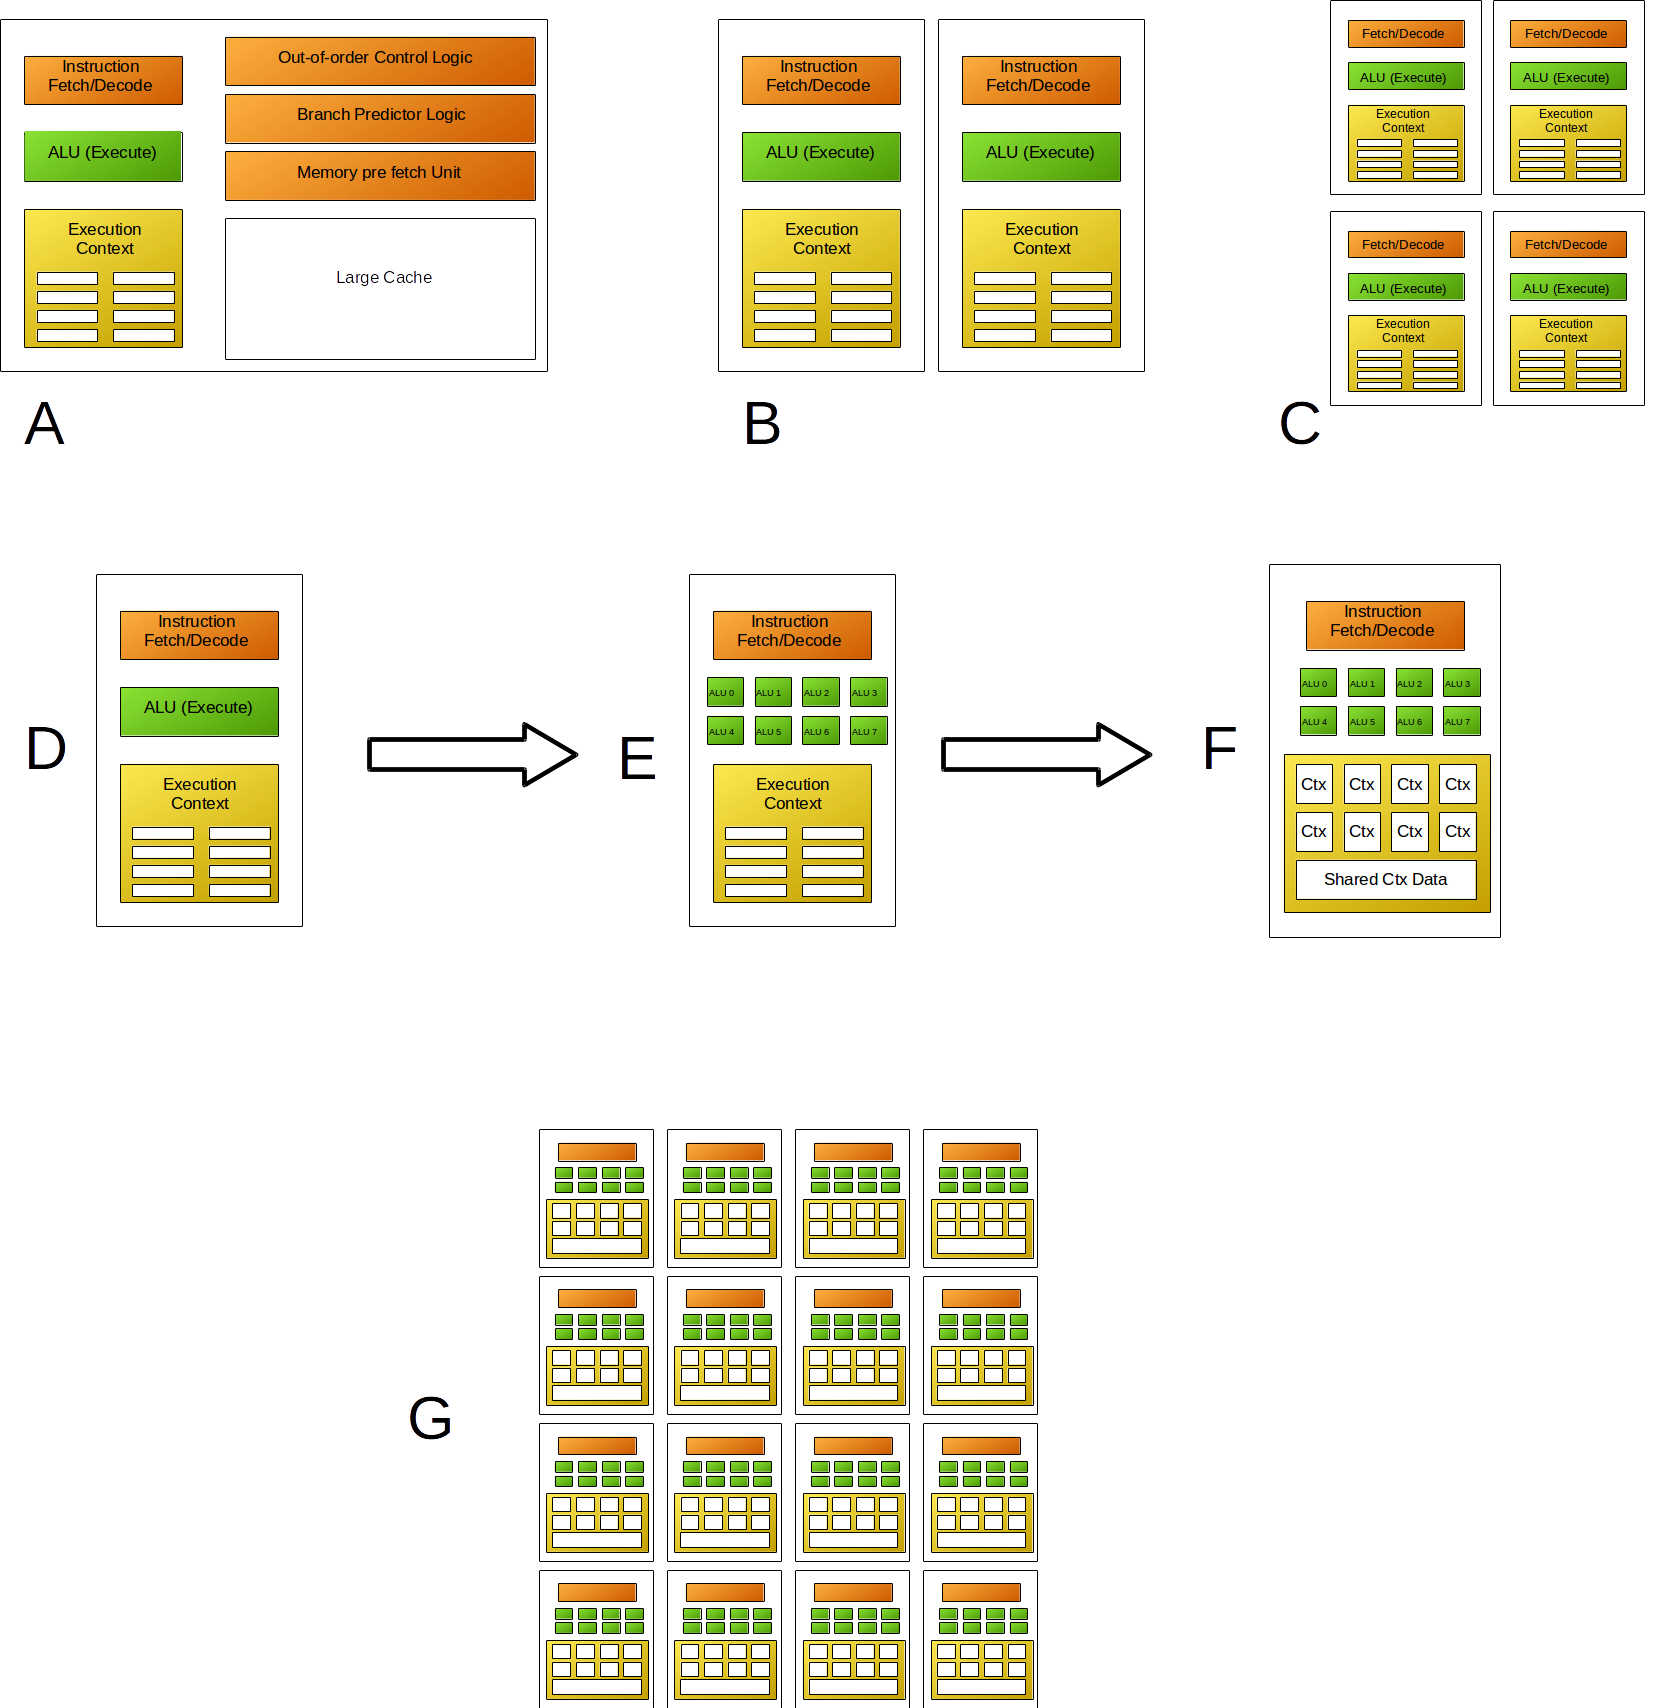
\includegraphics[width=0.8\textwidth]{CPU_to_GPU_metamorphosis.png}
    \caption{\gls{cpu} to \gls{gpu} metamorphosis. The first big idea that differentiates the \gls{cpu} in (A) from the \gls{gpu} in (B) is to slim down the footprint of each core removing all the units that help a single instruction to execute fast by getting rid of great part of the data path administration. Then since each simplified core takes less space it could be doubled up as in (C). Yet since in each pixel the program do the same sequence of operations, then \gls{gpu} rendering instructions streams are typically very similar and it is convenient to take superscalar strategy from \glspl{cpu} to the extreme in \glspl{gpu} (from D to E). In this way the \gls{gpu} ends up having one Instruction Fetch/Decode unit feeding for example 8 \glspl{alu}. This is the \gls{simd} model which shares the cost of the instruction streams across many \glspl{alu}. Finally each \gls{simd} group has to be provisioned with shared memory which has to keep a different context for each \gls{alu} operation as shown in (F). And since these are light weight cores then they can be massively allocated in a \gls{gpu} (G). \gls{cpu} cores do not have as many registers as the \gls{gpu} cores. As an example an Skylake core has 180 integer registers and 168 floating point registers while a Maxwell core has about 16k registers.}
    \label{fig:CPU_to_GPU_metamorphosis}
\end{figure}

Essentially, every operation on a \gls{gpu} is parallel. On a \gls{cpu} instead, the compiler has to actually be persuaded that an operation can be vectorized. In order to do that, the operation on the \gls{cpu} has to satisfy some criteria, for example, the data used for the operation has to be aligned in memory in a certain way. That is a pretty big restriction. At the core level every operation on a \gls{gpu} is vectorized, there is no alternative. There is no need of persuading the compiler on order to make vector operations on a \gls{gpu}. Then each \gls{cpu} core executes scalar or vector operations while each \gls{gpu} core only executes vector instructions. 

As a final aside note that matters for \gls{gpu} market and its relationship to \gls{dl} applications, NVIDIA--unlike AMD--has been pushing a lot in the last years for \gls{dl}. A lot of engineering effort has been invested by NVIDIA to make their hardware better suited for \gls{dl}. As an example of that we can cite the last Volta tensor cores which can do an $A*B+C$ 4 by 4 matrix operation completely in parallel. As a result NVIDIA is pretty dominant in \gls{dl} currently.





















































\subsection{Software approaches for \gls{dl} applications}

In reference to general purpose software tools which could be utilized for \gls{dl}, \gls{cuda} is a parallel computing platform and \gls{api} model created by NVIDIA. By means of \gls{cuda} developers can write code that looks like C but executes directly on \glspl{gpu}. Nevertheless,  writing \gls{cuda} code could end up being a real challenge, since it is very difficult to get a code with good performance, i.e. a code that takes the maximum advantage from all the \glspl{gpu}. Memory hierarchy has to be carefully managed trying to avoid cache mises and branch mispredictions. Then it is actually really hard to write performant \gls{cuda} code. As a result NVIDIA has released many libraries that implement common computational primitives which are highly optimized for \glspl{gpu}. Among such libraries, cuBLAS is an implementation of \gls{blas} on top of the NVIDIA \gls{cuda} runtime. It allows the user to access the computational resources of NVIDIA \gls{gpu}. Another library is cuFFT which is the NVIDIA \gls{cuda} \gls{fft} product. Such libraries are super optimized and run very well on \glspl{gpu}  getting very close to theoretical peak hardware specifications. Another \gls{gpu}-accelerated library is cuDNN which has primitives for deep neural networks. cuDNN provides highly tuned implementations for standard routines such as forward and backward convolution, pooling, normalization, and activation layers. So, in practice nobody tends to write his own \gls{cuda} code, instead everybody will typically be just mostly calling into extremely optimized software that other people have already written.

There is another language called \gls{opencl} which is a framework for writing programs that execute across heterogeneous platforms consisting of \glspl{cpu}, \glspl{gpu}, \glspl{dsp},  \glspl{fpga} and other processors or hardware accelerators. Yet, nobody has really spent a great effort trying to get optimized \gls{dl} primitives for this \gls{api}. As a result \gls{opencl} tends to be considerably less performant than the super optimized libraries in \gls{cuda}.

Referring to \gls{dl} frameworks more specifically, the landscape of those frameworks is very dynamic and great changes can be seen year after year. The first generation of \gls{dl} frameworks--which had wide adoption in the scientific community--was built mainly in academia. \gls{caffe} was from Berkeley, Torch was developed originally in \gls{nyu} in collaboration with Facebook and Theano was mostly built at University of Montreal. Yet, the next generation of \gls{dl} frameworks all originated in industry, \gls{caffe}2 and Pytorch are from Facebook while TensorFlow is from Google. It is an interesting shift in the landscape given in the last couple of years (Fig.~\ref{fig:ML_Frameworks}).

\begin{figure}[h!]
    \centering
    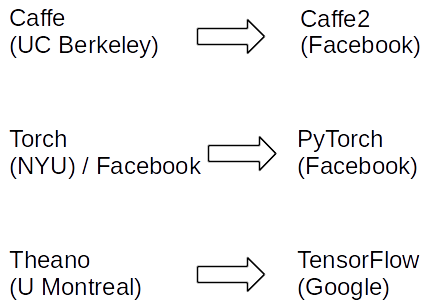
\includegraphics[width=0.35\textwidth]{ML_Frameworks.png}
    \caption{Interesting shift from Academia to Industry given in the last couple of years in the development of \gls{dl} frameworks.}
    \label{fig:ML_Frameworks}
\end{figure}

Whenever working on \gls{dl}, there is an important concept called \emph{computational graph} which computes all the functions to be run in the model. In the case of a linear classifier for example, certain data $x$ is combined with certain weights $W$ on the network using a matrix multiplier, there will be a computation of some kind of \emph{hinge loss} and a regularization computation too. Sticking together all these different operations emerges the graph structure of the network to be implemented. These graph structures can be pretty complex especially in the case of big \glspl{nn} with many different layers, many different operations and with many different weights spread throughout the network. Hence, the point of \gls{dl} frameworks is really simple. There are three main reasons that could lead to the use of one of those frameworks rather than just writing the code from scratch. 

\begin{itemize}
	\item The first reason is that these frameworks enable to easily deal and work with these big computational graphs without worrying about all those bookkeeping details.
	\item The second reason is that whenever working in \gls{dl} it will be always necessary to compute gradients, i.e. to compute some loss and then to compute the gradients about weights with respect to the loss. It would be better to make these operations as automated as possible. After all, nobody wants to struggle writing such code. Everyone wants the framework to handle all these backpropagation details. So the common scenario is writing only the forward pass of the network and having the backward pass sort of free without any significant addition to the code.
	\item And finally it is desirable to have all this stuff running efficiently on \glspl{gpu} so nobody have to worry to much about those low level hardware details such as cuBLAS and cuDNN in \gls{cuda}, moving data between the \gls{cpu} and the \gls{gpu}, etc. Everybody can keep all those messy details hidden by these tools which take care of them.
\end{itemize}

Suppose you want to execute a simple computational graph, one having some kind of matrix multiplications and additions. Using Numpy it is extremely simple, but suppose that you want to compute the gradients of a scalar output from the graph with respect to the input vectors. If you are working in Numpy you need to write this backward pass yourself. It can be kind of a pain and a little bit annoying and messy once you get really big and complicated graphs. The other problem with Numpy is that it does not run on \glspl{gpu}, i.e. Numpy is definitely \gls{cpu} only and you are never going to be able to experience or take advantage of these \glspl{gpu} accelerated speedups if you keep working in only Numpy. The goal of most \gls{dl} frameworks these days is to let you write code in the forward pass that looks very similar to Numpy, but letting to run it on \glspl{gpu} and automatically compute all the gradients. That is kind of the picture goal of most of these frameworks. So the general pattern in these frameworks is that you will have to define the variables initializing them and write the forward pass in a very similar fashion to Numpy, in the case of Pytorch the forward pass will be exactly the same than in Numpy. Then using a magic single line of code you will be able to compute all the gradients. The area of variable initialization is where an extremely simple tweak will allow you to cast your variables in order to instruct the compiler to run the code on \glspl{gpu}. In this way the frameworks solve two problems, first you are running your code transparently on \glspl{gpu} and second you are having the frameworks compute all the gradients automatically for you. So for example you will end up having a code written in TensorFlow or Pytorch which looks almost exactly the same than Numpy, which is great because Numpy is a beautiful \gls{api} and is really easy to work with, but you can also compute gradients automatically and you can run on \glspl{gpu} automatically too. 

The prototypical programing paradigm in TensorFlow is to divide the code into two major stages. First some code is devoted to define the computational graph and then, after the graph is defined, another code will run such graph over and over again feeding data into it in order to perform the necessary computations for the network. This is kind of the big common pattern in TensorFlow. First a bunch of code builds the graph and then another code run the graph reusing it many times. In the section that build the graph, firstly some variables are defined. For example some sets of vectors $x$s for the inputs and the intermediate outputs in the network and a some sets of $w$s for the different weights. In TensorFlow, \texttt{placeholder} and \texttt{Variable} objects are going to be the input nodes to the graph. They are like entry points where the graph is run feeding in data and putting them into these input slots.

When a placeholder or a Variable is defined, they are not allocated in memory. They are just defining those input slots in the graph. The difference between a placeholder and a Variable is the memory in which they will be allocated once the graph is run. In the case of a placeholder the consecutive runs will end up copying data back and forth between the \gls{cpu} and the \gls{gpu} in every time step. These objects are generally used to feed the networks with the input and the labels. A Variable on the other hand is a value that lives inside the computational graph--in \gls{gpu} memory--and will persist inside the graph across different time steps when such graph is run. These objects are generally used to store the weights of the network. Since all Variable data lives inside the computational graph, their initialization and update has to be specified inside the graph too in order to avoid great volumes of data movement between the \gls{cpu} and the \gls{gpu}. Those input slots--which are like symbolic variables--are going to be used to perform different TensorFlow operations. It is important to know that such lines of code are not actually computing anything, there is no data in the system since such code is just building up this computational graph data structure telling TensorFlow how is the structure of the network and which operations will be run once real data is put inside the graph. After the loss is computed, TensorFlow is generally instructed to compute all the gradients of the loss with respect to the weights $w$s in the graph using a single line of code. In all this configuration there is no actual computation happening, this is just sort of adding extra operations to the computational graph structure in memory which knows which operations has to be performed once the graph is run.

The next section of the code enters in a TensorFlow session that runs the computational graph and feed it with data. TensorFlow just expects to receive data from Numpy arrays in most cases. Then the different variables are stored in a dictionary and the graph is run with a special function of the session in which the user can specify which part of the graph actually wants as output. TensorFlow offers a lot of tools to make the programmer's life easier, from optimizers to run the complete graph even when it is only necessary to compute some intermediated value--TensorFlow is intelligent enough to implement only the necessary sections of the graph based in the outputs asked by the user--to tools to automate the computation of losses and higher level libraries to handle a lot of details to implement weights configurations of the different layers and activation functions. These libraries manage a lot of architectural details of the graph implementation.

There are many different higher level libraries that programmers build on top of TensorFlow. When working with higher level abstractions such as neural networks some abstract concepts like layers and weights could result really messy and inconvenient in a row computational graph without the use of some wrappers. So there are several packages to help to make the code stile cleaner. There are very popular packages such as Keras which is an open source neural network library written in Python and is capable of running on top of TensorFlow, Microsoft Cognitive Toolkit, or Theano. Keras is designed to enable fast experimentation with deep neural networks and focuses on being user-friendly, modular, and extensible. Keras builds all these computational graphs in the backend. It is important to take into account that there are a great variety of wrapper libraries which work on top of TensorFlow and that even people within Google cannot agree in which one is the right to be used. Tensorflow has also a distributed version which allows programmers to split one graph over multiple machines. As a side note, a lot in the design of TensorFlow is inspired in an earlier framework called Theano from University of Montreal. Generally speaking, the code from a Theano program ends up looking very similar to code in TensorFlow.

In reference to Pytorch, it is different from TensorFlow. There are three explicit different layers of abstraction inside Pytorch. Pytorch has an object called Tensor, which is just like a Numpy array, it is a imperative \texttt{ndarray} and does not know anything about \gls{dl} but it can run on \glspl{gpu}. Another object is the Variable object which is a node in a computational graph and builds up computational graphs, enables the use of gradients, etc. Finally, Pytorch also offers Module objects which are neural network layers which can store state or learnable weights and can be used to compose big networks in a modular way. Fig.~\ref{fig:Pytorch_TensorFlow} shows a simplified equivalence between Pytorch and TensorFlow in terms of the objects and libraries each tool utilizes.

\begin{figure}[h!]
    \centering
    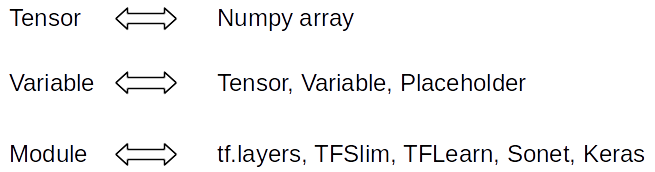
\includegraphics[width=0.5\textwidth]{Pytorch_TensorFlow.png}
    \caption{Row equivalence between Pytorch and TensorFlow objects and libraries.}
    \label{fig:Pytorch_TensorFlow}
\end{figure}

As can be seen in the figure, Pytorch is very simple and has less choices involved, which is better in some way since the user does not have to worry about--for example--which higher level wrapper to use. The major difference between Pytorch Tensors and Numpy arrays is that Pytorch Tensors run on \glspl{gpu}. Then having a code that is completely written in Numpy the programmer can make this code running on \glspl{gpu} simply by casting all the Numpy arrays to a different data type by means of just a single line of code. So Pytorch Tensors are Numpy arrays plus \glspl{gpu}, nothing specific to \gls{dl}. The next level of abstraction in Pytorch is the Variable. Moving from Tensors to Variables enables the built of computational graphs which are able to take gradients automatically. Then if \texttt{x} is a Variable, \texttt{x.data} is a Tensor and \texttt{x.grad} is another Variable containing the gradients of the loss with respect to that Tensor in a way that \texttt{x.grad.data} is a Tensor containing those gradients. Pytorch Tensors and Variables have the same \gls{api}, so in any code that works on Pytorch Tensors such Tensors can be casted to Variables and run exactly the same code but in this case the code is running a computational graph rather than just running this imperative operations. So the code ends of looking quite like the Numpy case except that all the gradients come for free.

In Pytorch you can define new autograd functions writing a class with forward and backward functions in terms of Tensors but most of the time you will probably not need to define your own autograd operations since such operations will be already implemented for you. In TensorFlow you can move to something like Keras or TFLearn which give you a higher level \gls{api} to work with rather than has to deal with those row computational graphs. In a similar way in Pytorch you will use the nn package which provides high level for working with layers and weights in networks. Like TensorFlow, Pytorch also has optimizers that--after computing the gradients--optimize all the parameters of the model for you. In Pytorch you will also define your nn Modules where a Module is kind of a neural network layer that can contain either other Modules or trainable weights. The characteristic scenario in Pytorch is defining your own class, defining your model that contains other Modules or not and then you will have some explicit training loop that updates the parameters of the model. One nice quality feature that is offered by Pytorch are DataLoaders. A DataLoader can handle data providing minibatching, shuffling, multithreading, etc for you. This tool can actually use multiple threads in the background to build minibatches offering a continuoum stream input data from disk. As an aside note Pytorch is kind of a newer updated version of an older framework called Torch. Pytorch is pretty much better in a lot of ways than Torch but they actually share a lot of the backend core for computing the Tensors and \gls{gpu} operations on Tensors. Some of the high level differences between Pytorch and Torch is that while Torch is based in Lua Pytorch is obviously based on Python and learning Lua could be kind of a turn off for some people, Torch does not have Autograd, but Torch is also older which could offer a more stable framework with less code to debug and maybe more examples to offer. Nevertheless, such scenario is changing quickly.

One important difference between Pytorch and TensorFlow is that in TensorFlow case you are first building an explicit graph and then running the graph many times. In Pytorch instead, you are building up a new graph every time you do a forward pass. This is one of the main distinguishing features between Pytorch and TensorFlow and this is called \emph{Static} vs \emph{Dynamic} computational graphs. This fact makes the code in Pytorch to look a bit cleaner in principle but it has other very important implications. For a very simple feed-forward neural network this issue does not make a huge difference, the code ends up looking very similar between the two frameworks and it runs in a similar way too. To talk a little bit about those two scenarios, in the static framework since the graph is built just once and then reused many times the framework may have the opportunity to do all kind of optimizations on the graph, i.e. fusing some operations, reordering some other operations, figuring out the most efficient way in which to operate the graph in order to make it really efficient. Since you are going to reuse the graph many times, that optimization process could be expensive at first but that cost could be amortized with the speedup you have gotten when you run the graph many times. As can be deduced, those kind of expensive optimizations could not be very well suited for dynamic graphs specially making reference to the natural approach of rebuilding the graph in each iteration. Another subtle point in terms of static vs dynamic is the idea of serialization. With static graphs once you build the graph you can have that data structure in memory which represents the complete structure of your network. Then you can take that data structure and just serialize it at the disk saving it in some file in order to reload it later to run such computational graph without access to the original code that built it. This could be kind of an advantage for a deployment scenario where you can train your network in Python because it is maybe easy to work with but then, after you serialized that network you can deploy it maybe in a \CC~scenario in which you will not need to use the original code that built the graph. In a dynamic graph scenario since you are interleaving those stages of graph building and graph execution you will end up needing the original code to reuse that model in the future.

An advantage for dynamic graphs--on the other hand--is that this framework makes your code much cleaner and easier to comprehend. For example, inserting conditionals in the graph section of the code is very straightforward in Pytorch--exactly as it is in Numpy. In TensorFlow the situation is more complicated since you build the graph once and these control flow operations will need to be explicit operators in the graph. Since you build all the graph once all the potential paths from the control flow need to be dug into the graph at the time you construct it--before you ever run it. Then any control flow operation in TensorFlow cannot be a simple Python control flow operation. It will be necessary to use kind of special TensorFlow operations. As can be deduced, static graphs can also be very problematic in recursive loops were the input to the loop could vary its length a lot in each iteration. Summarizing, we end up having the sense that TensorFlow is almost building its own entire programming language, using the language of computational graphs. In this way, any kind of control flow operator needs to be rolled into the computational graph so you will end up learning a complete set of control flow operators--a new language. Finaly there actualy is a library called TensorFlow Fold that is another kind of layer on top of TensorFlow that lets you implement dynamic graphs.

In reference to Caffe, this is different from the other \gls{dl} frameworks in which--in many cases--you can train networks without writing any code yourself. As a first step you will convert your data into some format such as LMDB. There are some scripts inside Caffe for that. Then you will need to define a text file (prototxt) which sets the structure of the computational graphs which is completely described in this text file. One downside of these files is that can be really ugly for very large networks. A ResNet with 152 layers results in a prototxt file with 6775 lines. Obviously, people are not writing it by hand and they are writing Python scripts to generate these prototxt files which means that they are running into their own computational graph structure which ends up not being a really good idea. Instead of having some optimizer objects Caffe has some kind of solver which defines the learning rate, the optimization algorithm to use, etc. Finaly, once you have done all those things you can run the Caffe binary with a \texttt{train} command and all happens magically. As a general evaluation Caffe could be good for feedforward models, is good for production scenarios since it does not depend on Python. Nevertheless Caffe is not being used for research very much, but it is pretty commonly used in industry or production. In reference to Caffe2, it is a successor from Caffe from Facebook that uses static graphs as TensorFlow which prevents you from writing those scripts in order to generate prototxt files. In Caffe2 you can define your computational graph structures all in Python using an \gls{api} that looks like TensorFlow but you can serialize this computational graph structure to a prototxt file. So you do not need the original training code in order to deploy a trained model.

One last interesting thing is the way in which companies approach the development of those frameworks. Google tends to have one major \gls{dl} framework which is TensorFlow while Facebook has two which are Pytorch and Caffe2. These are different philosophies, on the one hand, Google tries to build one framework to rule them all and which maybe works for every possible scenario for \gls{dl}. This philosophy is good because it is consolidating all efforts onto one framework that works on many different scenarios--including distributed systems, production, deployment, mobile, research, etc--and prevents people from learning many languages since there is just one framework for everything. On the other hand, Facebook is taking a different approach where Pytorch is really more geared towards research since in terms of writing research code and quickly iterating through ideas is super easy in Pytorch but for things like running in production or in mobile devices Pytorch does not have a lot of great support. Instead Caffe2 is kind of geared towards those more production oriented use cases. 




































%\subsection{Human Engineered Features}

%Among the computational theories developed to understand human phonetic acquisition, some models bypass the initial speech signal processing and, instead of dealing with the complexity and variability of real speech at the prelexical level, they use an artificial, often hand-crafted,  idealized discrete (prelexical) representation of the acoustic signal as an input to the lexical level \cite{scharenborg_2010}. In other works \cite{dominey_2000}, although some biological observations are made, the input components are syllable representations from specific corpora.

%In the works by de Boer and Kuhl \cite{boer_2003} and Vallabha, McLelland, Pons, Werker and Amano \cite{vallabha_2007}, the models classify some vowels through statistical mechanisms which consider formant components and \gls{vl}. In Toscano and McMurray \cite{toscano_2010}, statistical methods are used to classify consonantal phonetic characteristics, by means of \gls{vot}, \gls{vl}, pitch and first formant onset frequency.

%In Kouki et al. \cite{kouki_2010}, the use of \gls{mfcc} strategy presupposes a more biologically accurate input stream. In a subsequent work, Kouki et al. \cite{kouki_2011}, designed a method to separate “stable” and “dynamic” speech patterns.

%The statistical methods used in such works make different features extracted from acoustic speech signals interrelate. Those features are carefully weighted by means of human engineering and domain expertise, which evaluate their relevance in order to include them in the computations. Some features, as \gls{vl} and \gls{vot}, refer to highly abstract dynamic characteristics which are taken as available parameters without any previous natural processing.

%\subsection{Machine Engineered Features}

%The possibility of the existence of other features which can escape from human expertise and the fact that some hidden features could be a constituent part of those abstract features evaluated by humans allowed the advent of deep learning approaches which have fairly gained outstanding interest as a way of building hierarchical representations from unlabeled and labeled data.

%Referring to multilayer supervised learning, the fact that such architectures can be trained by simple stochastic gradient descent, and that they work remarkably well, was discovered independently by different groups during the 1970s and 1980s \cite{noauthor_9_nodate,noauthor_parker_nodate,lecun_procedure_1985,rumelhart_learning_1986}.

%However, a first widespread acceptance hit of these architectures had to wait until 2006 \cite{hinton_what_2005,hinton_fast_2006,bengio_greedy_2006,ranzato_efficient_2006} when a group of researchers introduced deep unsupervised learning procedures which initially pre-train the network for finally fine-tune it by means of standard backpropagation \cite{bengio_greedy_2006,ranzato_efficient_2006,hinton_reducing_2006}. It returned record-breaking results--as a constituent part of a complete system--on a standard speech recognition benchmark for small \cite{mohamed_acoustic_2012} and then for large \cite{dahl_context-dependent_2012} vocabulary tasks.

%Despite of the success in the application of \glspl{cnn}--since 2000--to  traffic sign recognition \cite{ciresan_multi-column_2012}, segmentation of biological images \cite{ning_toward_2005,turaga_convolutional_2010}, detection of faces, text, pedestrians and human bodies in natural images \cite{sermanet_pedestrian_2012,vaillant_original_1994,nowlan_convolutional_1995,garcia_convolutional_2004,osadchy_synergistic_2007,tompson_efficient_2014}, face recognition  \cite{taigman_deepface:_2014} and despite of its successful applications in technology, including autonomous mobile robots and self-driving cars \cite{hadsell_learning_nodate,farabet_scene_2012} as well as natural language understanding  \cite{collobert_natural_2011} and speech recognition \cite{noauthor_deep_nodate}, those approaches had to wait until 2012 to be widely accepted by the mainstream computer-vision and machine-learning communities, when in the ImageNet competition in 2012 deep convolutional networks achieved spectacular results, almost doubling the accuracy rates respecting to the best competing approaches \cite{krizhevsky_imagenet_2012}.

%In reference to distributed representations in language processing, and in the context of very large corpora in real text, deep neural networks are trained to predict the next word from a chain of words by taking into account the most recent words in the neighborhood inside the sequence. Some times the only premise is to take into account the previous and the next words in relation to the word that want to be predicted. It is striking that from too simple premises can arise insightful distributed semantic representations in which the learned word vectors for Tuesday and Wednesday--for example--are very similar, as are the word vectors for Sweden and Norway  \cite{bengio_neural_2003}. Semantic features learned by such networks are not determined by experts in advance, instead, they are automatically discovered by the neural network.

%Very simple mechanisms carried out by \glspl{rnn} for sentence translation and automatic image caption generation raised incriminating doubts about the need of internal symbolic expressions manipulated by inference rules. In that sense, it is highlighted that everyday reasoning might involve many simultaneous analogies, each contributing with plausibility to a conclusion \cite{noauthor_metaphors_nodate,rogers_precis_2008}.

%\gls{lstm}--an improved version of conventional \glspl{rnn}--can be applied in the implementation of complete speech recognition systems  \cite{graves_speech_2013} and has also been used for the encoder and decoder networks at machine translation  \cite{sutskever_sequence_2014,cho_learning_2014,bahdanau_neural_2014}. Turing machines and memory networks are \gls{lstm} improvements that have been used for tasks that would normally require reasoning and symbol manipulation  \cite{graves_neural_2014,weston_memory_2014,weston_towards_2015}.

%\subsection{Biological Plausibility}

%Even though \glspl{cnn} are inspired by the phenomena developed by simple and complex cells in the visual pathway and is reminiscent of the LGN–V1–V2–V4–IT hierarchy in the visual cortex ventral pathway  \cite{felleman_distributed_1991}, the mainstreams in the development of such tools has virtually ignored biological counterparts as to find support which explains--at least in part--the outstanding performance of such approaches. In that sense,  and in terms of the enormous influence of deep supervised neural networks during the last years, there are researchers who support the hypothesis that backpropagation could be carried out in neural tissue \cite{guerguiev_towards_2017}. In that work, the credit assignment problem is explained in terms of biological plausibility implementing a network which--layer by layer--clusters visual information with increasing abstract representations of digit categories. 

%In another proposal \cite{hinton_matrix_2018,sabour_dynamic_2017}, Geoffrey Hinton tries to tackle biological plausibility in a top-down fashion highlighting important drawbacks in \glspl{cnn} as the lack of pose (translational and rotational) relationship between simpler features that make up a higher level feature and the fact that max pooling provides an artificially forced invariance to the network at expenses of valuable information. Inspired by how computer graphics construct a visual image from its internal hierarchical representation of geometric data, Hinton instead alleges that our brain do kind of a reverse rendering process--inverse graphics as he calls it--from visual information received by eyes. For Hinton, our brain extracts a hierarchical representation of the world and tries to match it with already learned patterns and relationships previously stored in the brain. The main idea behind this theory is that representation of objects in the brain does not depend on view angle and in this way they have a more naturally sourced invariance property. This network has reached state-of-the-art performance in a simple data set using just a fraction of the training examples that would need a \gls{cnn}. In this sense, the capsule theory is much closer to what the human brain does in practice.  Beyond this encouraging outcome, current implementations are much slower than other modern deep learning models in order to be trained.

%Biological entities discover the structure of the world without being told how, interacting with it and receiving reward and punishment in the best cases--reinforcement learning--while in other cases learning without any clue beyond the statistical structure in the data itself in a completely unsupervised fashion. Reinforcement learning seems to be the conditions under which animals are most often exposed to.  In that sense, a combination of supervised learning from human expert games, and reinforcement learning from games of self-play was used to train AlphaGo, a \glspl{dnn} \cite{silver_mastering_2016} that achieved a 99.8\% winning rate against other Go programs, and defeated the human European Go champion by 5 games to 0. Then, in \cite{silver_mastering_2017} AlphaGo became its own teacher by means of an algorithm based solely on reinforcement learning. Without human data, guidance or domain knowledge beyond game rules, this neural network was trained to predict AlphaGo’s own move selections and also the winner of AlphaGo’s games. This neural network improves the strength of the tree search, resulting in higher quality move selection and stronger self-play in each iteration. Starting tabula rasa, the new program AlphaGo Zero achieved superhuman performance, winning 100–0 against the previously published, champion-defeating AlphaGo.

%Beyond the fact that reinforcement learning could be thought as an ubiquitous mechanism in complex biological systems, it is important to highlight that unsupervised techniques could lead the learning processes in many cases in biological agents too. Regarding this, Jeff Hawkins et al. \cite{noauthor_why_nodate} have developed a computational approach which gather precise biological properties from cortical tissue. This work shows how a biologically detailed model of pyramidal neurons with thousands of synapses and \glspl{sdr} can learn transitions of patterns and can form a powerful and robust sequence memory \cite{noauthor_htm_nodate}. They propose that such form of sequence memory could be a universal property of all neocortical tissue. The same group is currently developing a compelling approach \cite{noauthor_theory_nodate} by means of a network model that learns the structure of objects through movement. In such research it is foreseen that grid cells could lead that acquisition of the structure of the world in the mammalian cortex. 































\section{\gls{cstm}}
%\section{Algorithmic Implementation}

%\subsection{Data Flow}

Our \gls{cstm} simulates a patch of cortical tissue in the mammalian brain~\cite{dematties2018}. Fig. \ref{fig:DataFlow} shows the data flow of the information converging to the \glsfirst{el}--the main algorithm in this model. Sound waves are firstly processed by the \gls{mrstsa} algorithm. We followed the main guidelines in the implementation of the cortical section of Chi T. et al. \cite{chi_2005} model in order to implement the \gls{mrstsa} algorithm.

\begin{figure}[h!]
    \centering
    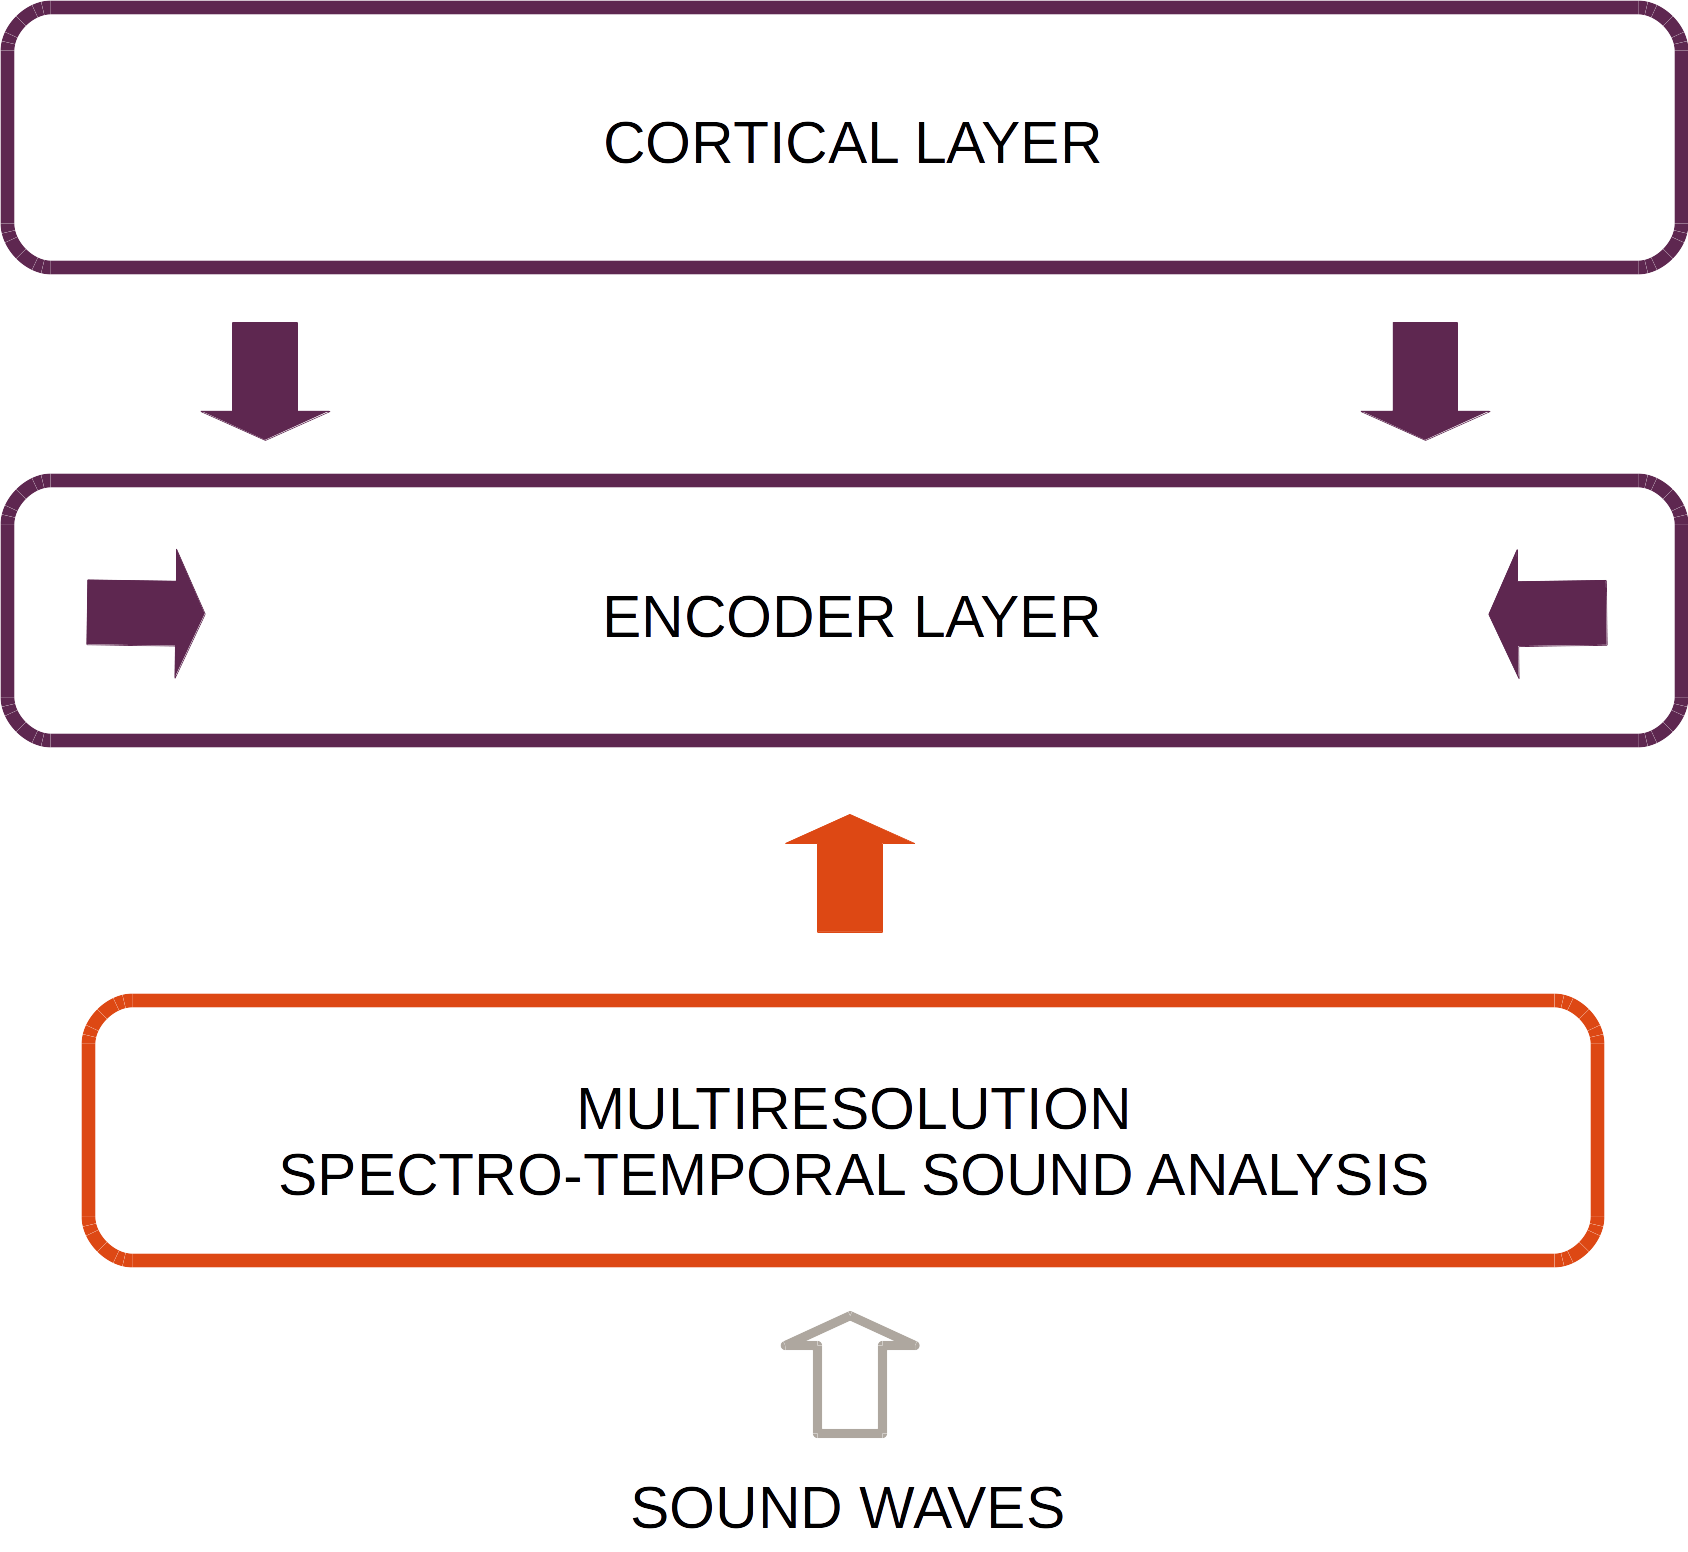
\includegraphics[width=0.3\textwidth]{DataFlow.png}
    \caption{Firstly, the \gls{mrstsa} processes the sound waves in a sequence of temporal windows and obtains a sequence of arrays of real numbers. Such sequence of arrays is received by the \gls{el} by means of proximal afferent connections. The \gls{el} also receives distal lateral connections which bring information from its self processing and distal apical connections which bring information from other cortical layers above the \gls{el}.}
    \label{fig:DataFlow}
\end{figure}

%We simulate pyramidal cells with proximal connections from afferent dendritic branches and distal connections from lateral and apical dendritic branches (Fig. \ref{fig:Pyramidal_Cell}).

%\begin{figure}[h!]
    %\centering
    %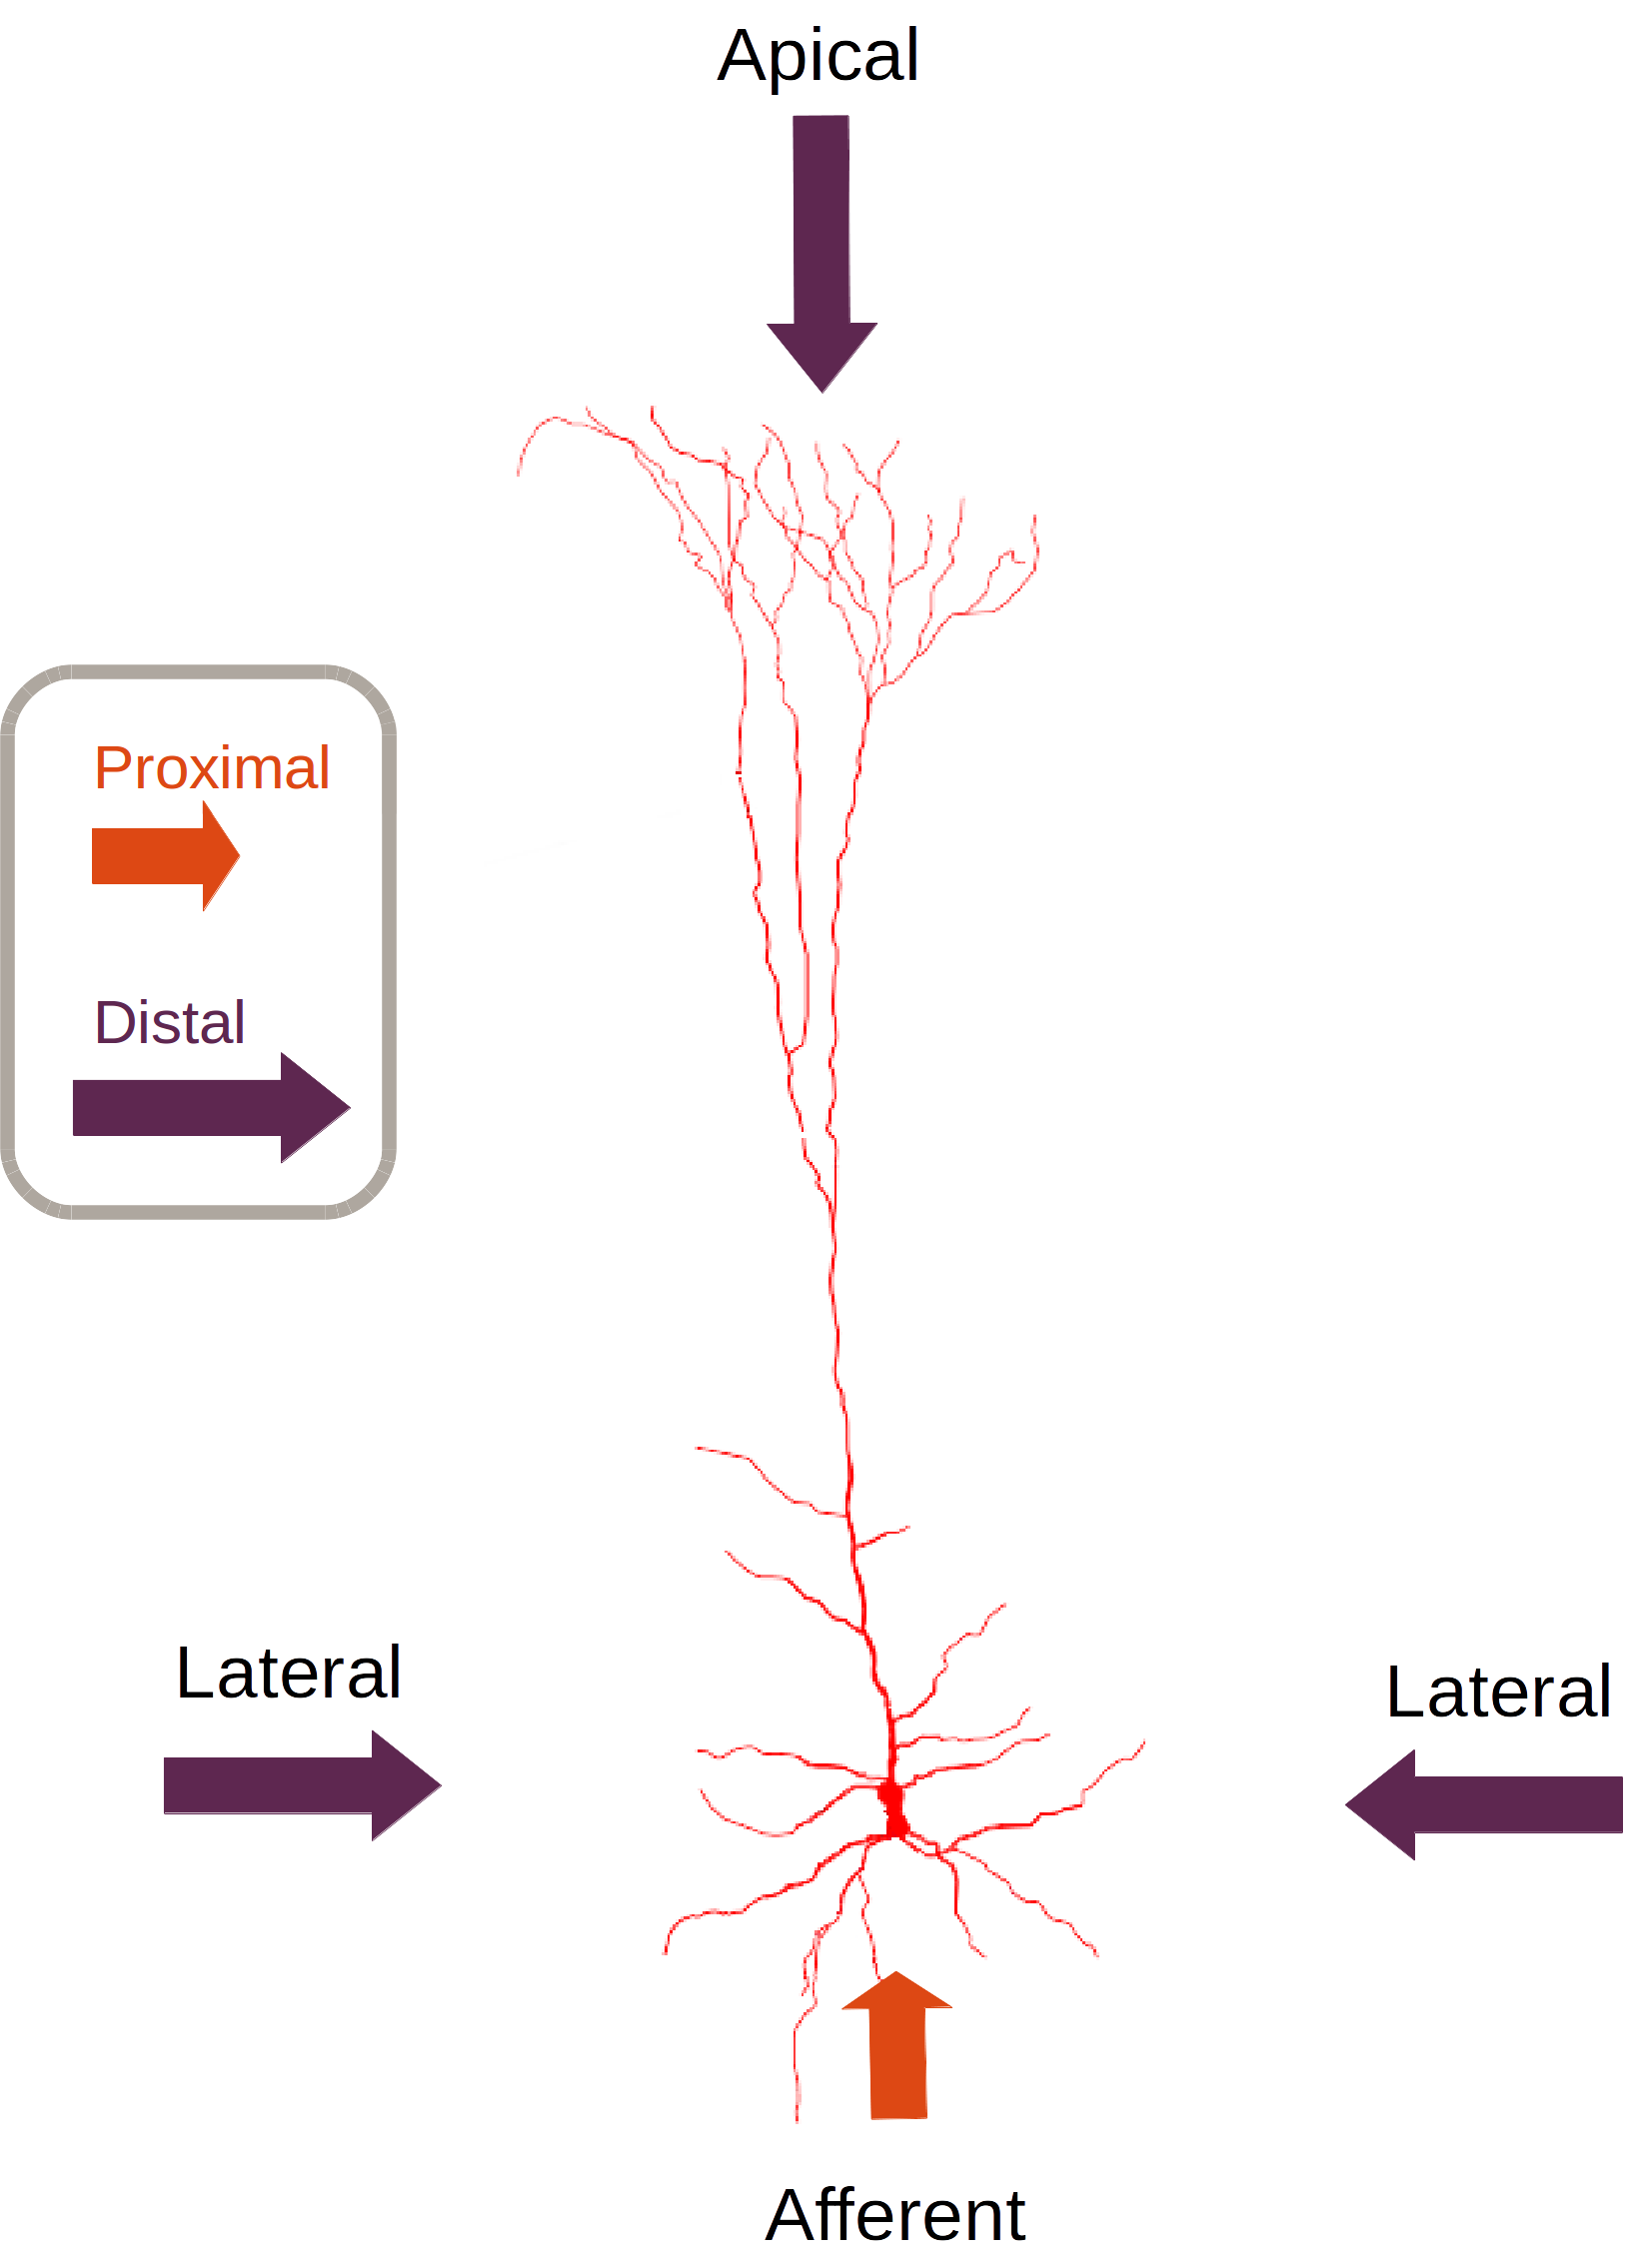
\includegraphics[width=0.4\textwidth]{Pyramidal_Cell.png}
    %\caption{Connectivity profile of a pyramidal neural unit in the \gls{el}. Proximal connections are composed only by afferent connections from the \gls{mrstsa} algorithm while distal connections are composed by lateral and apical connections from neighboring columns and    from columns in another cortical layer above respectively. Adapted from (Fabuio - Own work, CC BY 4.0, \url{https://commons.wikimedia.org/w/index.php?curid=60707501)}}
    %\label{fig:Pyramidal_Cell}
%\end{figure}

The \gls{el} simulates a patch of cortical tissue using an n-dimensional array of complex structures called \glspl{csom} that simulate \glspl{cc} in the brain. The \gls{el} generates \glspl{sdr} \cite{ahmad_2016} from the inputs delivered by the \gls{mrstsa} stage and from the activation history in its own \glspl{cc}. 

Each cell unit in a \gls{cc} has two types of dendritic branches; proximal and distal. Proximal and distal dendritic branches lead to proximal and distal connections in a cell unit respectively~\cite{dematties2018}. Neural units in the \gls{el} simulates pyramidal cells in cortical tissue in the brain (Fig \ref{fig:Pyramidal_Cell}). 

\begin{figure}[h!]
    \centering
    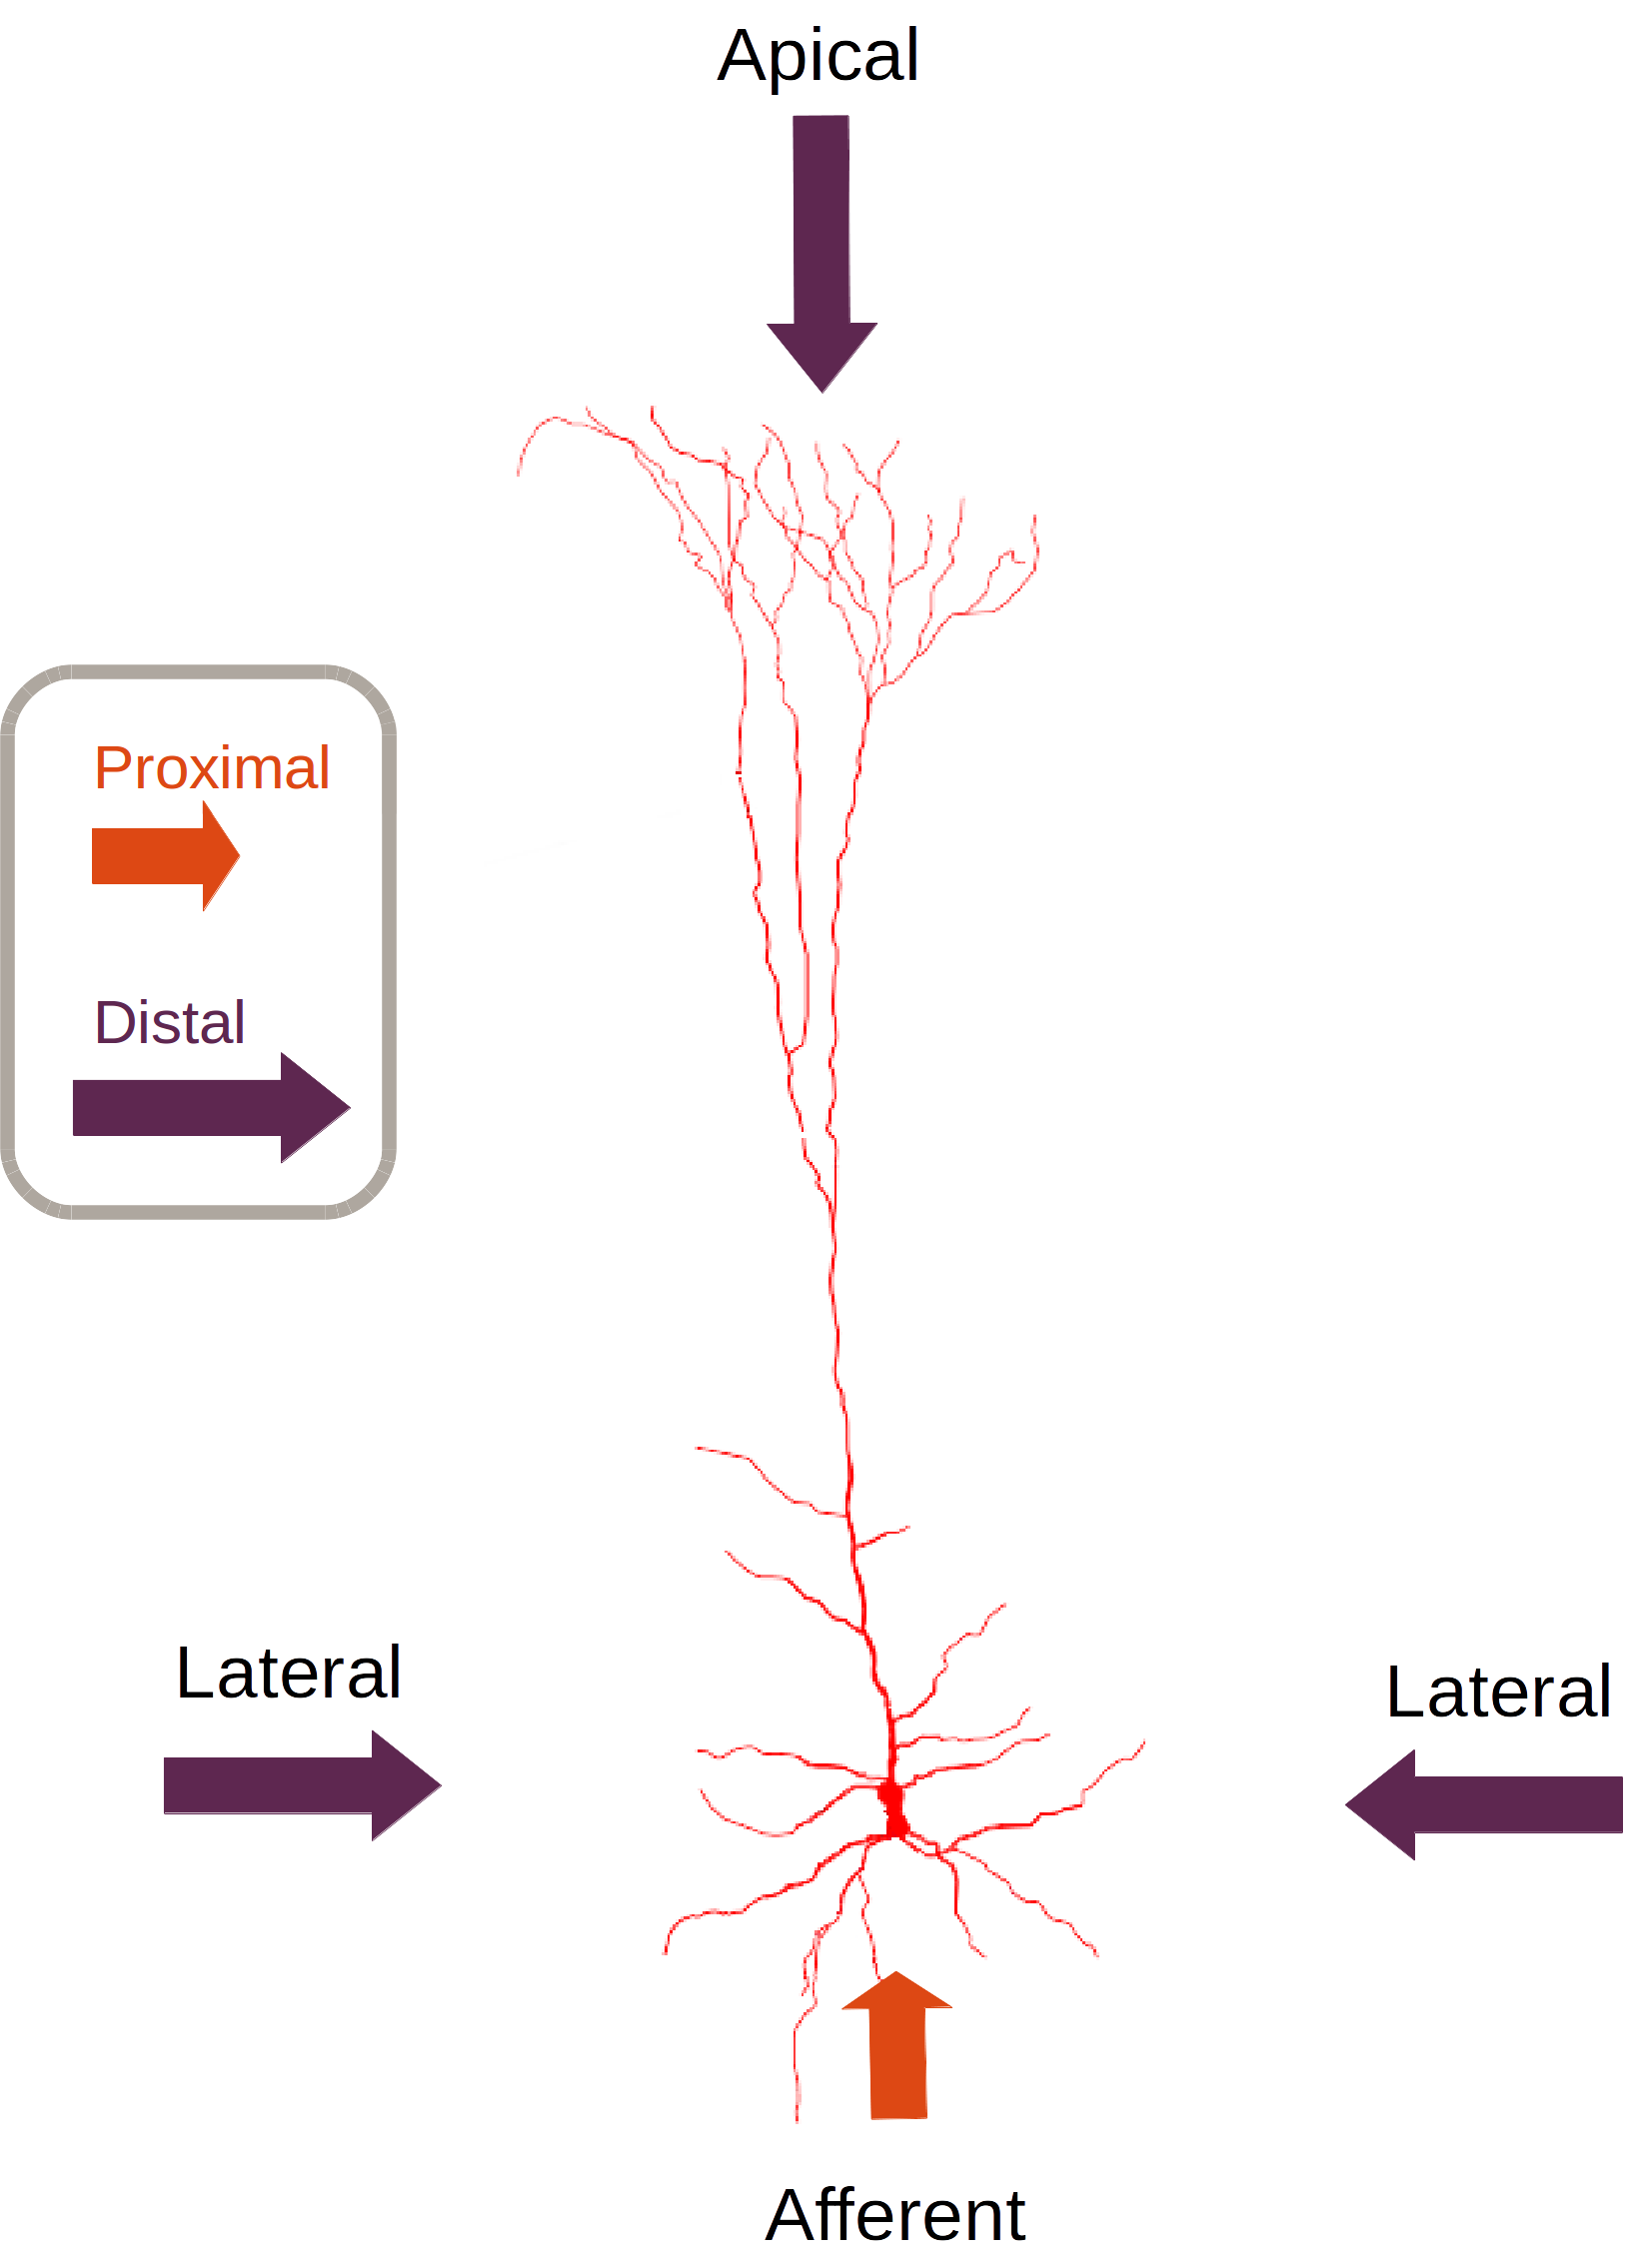
\includegraphics[width=0.3\textwidth]{Pyramidal_Cell.png}
    \caption{Connectivity profile of a pyramidal neural unit in the \gls{el}. Proximal connections are composed only by afferent connections from the \gls{mrstsa} algorithm while distal connections are composed by lateral and apical connections from neighboring columns and    from columns in another cortical layer above respectively. Adapted from (Fabuio - Own work, CC BY 4.0, \url{https://commons.wikimedia.org/w/index.php?curid=60707501)}}
    \label{fig:Pyramidal_Cell}
\end{figure}

%Each cell unit in a \gls{cc} has two types of dendritic branches; proximal and distal. Proximal and distal dendritic branches lead to proximal and distal connections in a cell unit respectively. Proximal and distal connections produce different effects on a neural unit's plasticity and activation. Neural units in the \gls{el} simulates pyramidal cells in cortical tissue in the brain. Fig \ref{fig:Pyramidal_Cell} shows the connectivity profile in such units. 

%Each \gls{cc} in the \gls{el} is connected to the \gls{mrstsa} below by means of afferent connections. It is also connected to neighboring \glspl{cc}--including possibly itself--in the \gls{el} by means of lateral connections and to \glspl{cc} from other \glspl{cl} above by means of apical connections. Such connection scheme is shown in Fig \ref{fig:DataFlow}.

%Similar afferent stimuli activate clusters of neurons with proximal physical locations in a \gls{cc} in the same way that afferent information activates the mini columns found in cortical tissue. Afferent information activates different clusters of units in a \gls{cc} establishing a first and raw approximation of the phonetic features abstracted from the input auditory stream. Our model fine-tunes such raw features by means of previous contextual activations produced in the same and/or in neighboring \glspl{cc}. Such contextual information is sent to each \gls{cc} by means of lateral distal dendritic branches which work as independent processing elements in a cell. Current activation in such dendritic elements will affect the way in which cells receives future afferent information. Such connections damp the activity of some units allowing only the precise activations of specific neural units in an afferently excited \gls{cc}. Such precise activations match the sequential paradigms learned by the network.

%Recent findings in neuroscience \cite{Marques2018} support the idea that feedback could potentially enhance visual representations in time and space damping the activity of certain cells while allowing the activation of others in agreement with its predictions. In this paper we only implement lateral connections since there are no upper layers from which to bring apical information in the present implementation.

%Novel computational theories have posited a feasible explanation about the role of distal synapses related to \gls{nmda} phenomenon \cite{hawkins_2016} by combining it with \glspl{sdr} \cite{ahmad_2016}. In our model, we adopt a similar approach to the one in \cite{hawkins_2016} in which current activation patterns produce partial depolarization of certain cells by means of distal dendritic branch connections. A state of partial depolarization is sustained in time in some cells within future afferently excited clusters of neurons. Partially depolarized cells fire in advance with respect to other cells in the excited clusters, thereby preventing other cells from firing by means of proximal lateral GABAergic inhibition, obtaining in this way, \glspl{sdr}.

%In addition, we simulate the growth of distal dendritic branch synapses by means of \gls{stdp} mechanisms together with homeostatic regulations. In this way, distal synapses will be established only among pyramidal cells with sequential patterns of activation. Afferently excited clusters which do not have partially depolarized cells, will fire together producing a \gls{mfe} (lack of inhibition) as a response to a prediction fault (unexpected sequential stimuli in the stream of data); otherwise they will respond with normal firing events (inhibition and therefore \glspl{sdr}) when the sequential stimulus is correctly predicted.

%\glspl{sdr} exhibit interesting mathematical properties which give them high noise rejection and fault tolerance \cite{ahmad_2015}. These are typical characteristics in cortical tissue where individual cells are far from 100\% reliable and the cells die and regenerate continuously. To simulate this phenomenon, we incorporate stochastic characteristics by which neural cells inside afferently activated clusters are chosen to be active by a discrete distribution whose probabilities are determined by the afferent excitability of individual cells during training.

%Hence, the evolution of our network does not predetermine a neuron to fire but biases its probability of doing so during training. Additionally and under specific conditions, afferent dendritic arborizations activate themselves at random with levels whose boundary values are established by learning. 

%It has been shown that overfitting--a phenomenon in which a statistical model describes random error or noise instead of the underlying relationship--is greatly reduced by stochastic properties in training procedures applied to neural networks (dropout)~\cite{JMLR:v15:srivastava14a}.






















%\subsection{\glsfirst{mrstsa}}
%\label{mrstsa}

%We implemented the initial stage in the \gls{mrstsa} with the application of \gls{fft} to the audio vector with a different sample window for each resolution. We then extracted the power spectral density from each resolution. We applied \gls{fft} to the audio files with a sample period of 8 milliseconds, to that end we used the FFTW package \cite{FFTW05, fftw} with time windows of 8, 16, 32, 64 and 128 milliseconds. In this way we obtained a multiresolution spectral analysis of the audio signal, with high spectral and low temporal resolution for wider sample windows and vice versa. Such different time windows in the \gls{fft}, incorporated--at the same time--leakage low-pass filters with a time constant for each resolution accounting for decrease of phase-locking in the auditory nerve. We then applied a \gls{mfb} with 128 elements to each spectrum in order to represent the spectral analysis performed by the cochlear filter bank (Fig.\ref{fig:MRSTSA}).

%\begin{figure}[h!]
    %\centering
    %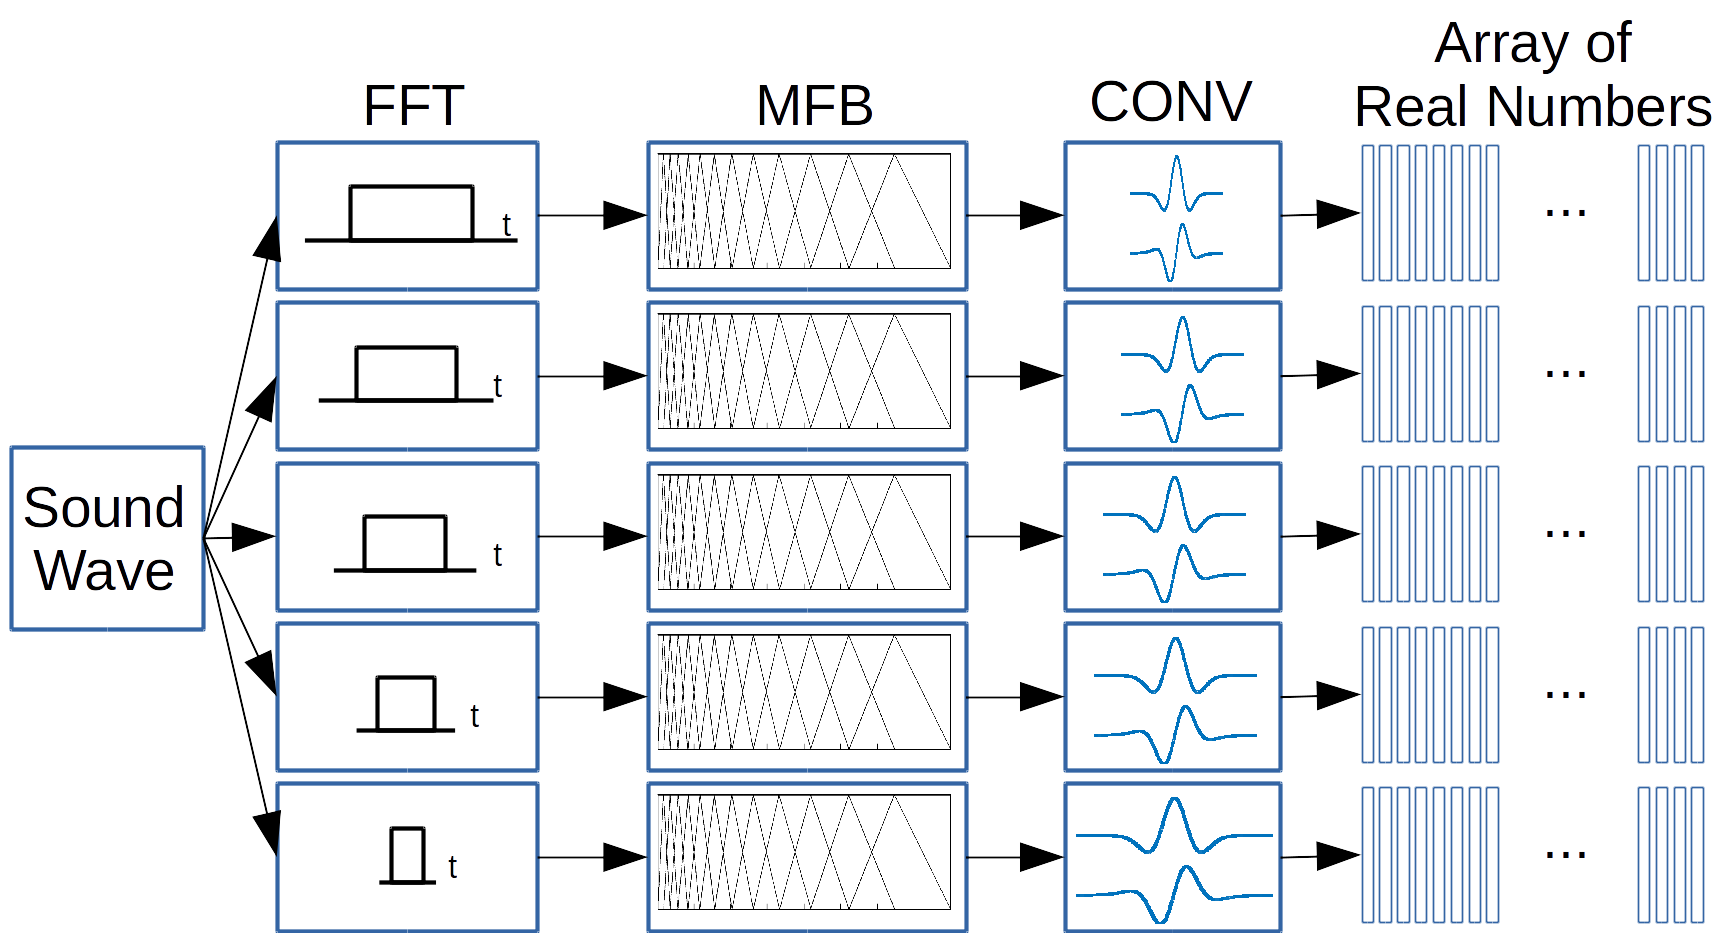
\includegraphics[width=0.8\textwidth]{MRSTSA.png}
    %\caption{\glsfirst{mrstsa} algorithm. Sound waves are processed by \glspl{fft} with different time windows, then each spectrum is processed by
    %a \glsfirst{mfb} and each resolution is convolved with a complex signal with a different coefficient. Then, each filter coefficient
    %is obtained computing the modulus from the convolution and then applying a authomatic gain control.}
    %\label{fig:MRSTSA}
%\end{figure}

%Then, we convolved each resolution obtained in the last step along its tonotopic axis with a complex multiresolution function whose real part was a symmetric Mexican hat function and its imaginary part was its antisymmetric Hilbert transform. The function coefficients are 10 for the 8 ms time window, 8 for the 16 ms time window, 6 for the 32 ms time window, 4 for the 64 ms time window and 2 for the 128 ms time window (Fig.\ref{fig:MRSTSA}). With this strategy we incorporated the phenomena of symmetry \cite{shamma_1993}, bandwidth \cite{schreiner_1990} and frequency modulation selectivity \cite{shamma_1993,heil_1992,mendelson_1985} found in \gls{a1} and incorporated in the original algorithms \cite{wang_1995}.

%We obtained the magnitude of each convolution and applied normalization to each time window as a mean of automatic gain control in order to prioritize the information delivered by the spectral configuration and not the absolute values delivered by the filters. By means of this constraint we account for the mechanical and chemical properties of hair cells in the mammalian inner ear which constitute a transduction mechanism that appears to adapt to recent stimulus history in a way that can affect its gain \cite{eatock_2000,holt_2000,le_goff_2005}. We decided to be conservative, not including sound intensity dimension but just the shape of the filter responses.

%By this procedure we obtained from the audio file a multiresolution spectro-temporal response composed by an array of 128 columns--one column per filter--and 5 rows--one row per resolution--with real numbers which range from 0 to 1, for each time step.




















%\subsection{\glsfirst{el} proximal dendritic connections plasticity}
%\label{proximal_dendrites}

%In reference to proximal connections in the \gls{el}, each neural unit in a \gls{cc} has the same set of proximal connections to the \gls{mrstsa} (Fig. \ref{fig:DataFlow}). This situation is depicted in Fig. \ref{fig:EncoderProximalConnections} and such connections constitute a multidimensional space of real numbers (Fig. \ref{fig:MRSTSA}). In order to acquire the statistical distribution in such multidimensional real space we use a multidimensional \gls{som} in each cortical column whose algorithm is depicted in Alg. \ref{csom_proximal_synapses}. Each neural unit has a synaptic weight per input dimension and the set of synaptic weights in a neural unit determines its position in the input space. Such synaptic weights try to copy the input vector events as they happen in the input space. 

%\begin{figure}[h!]
    %\centering
    %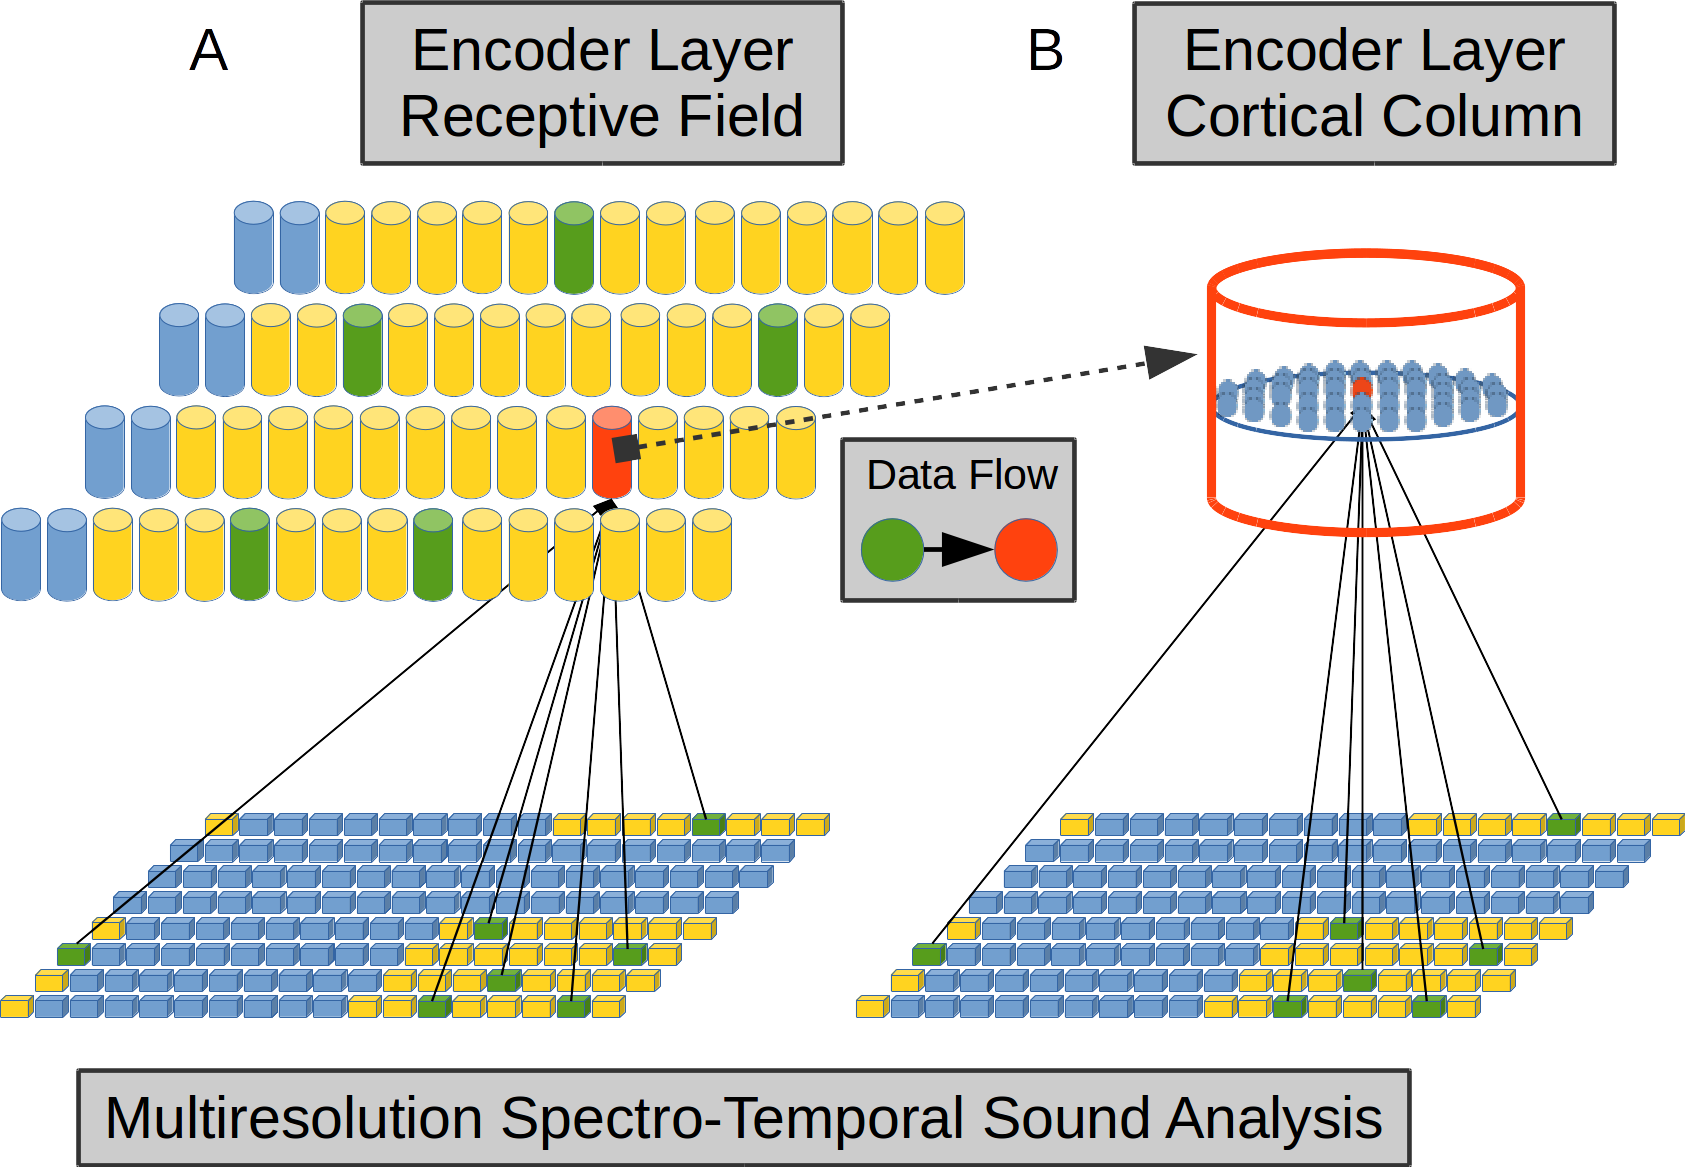
\includegraphics[width=0.6\textwidth]{EncoderProximalConnections.png}
    %\caption{\glsfirst{el} proximal connections. Each \gls{cc} in the \gls{el}--exemplified here in red--has its receptive field over the \gls{mrstsa}--in yellow.
    %(A) A set of \gls{mrstsa} components--in green inside the receptive field--is randomly chosen to be connected with such \gls{cc}.
    %(B) Each neural unit in such \gls{cc} is connected with the same set of \gls{mrstsa} components.}
    %\label{fig:EncoderProximalConnections}
%\end{figure}

%\begin{algorithm}
	%\caption{\texttt{Plasticity in Proximal Synapses}. This algorithm (a \gls{som}) is an unsupervised clustering algorithm which distributes a continuous multidimensional distribution in a discrete multidimensional distribution of units \cite{Kohonen:1989:SAM:69371, kohonen_2082}. In this way we ended up with an array of units of $m$ dimensions in which each unit represents a set of vectors from the continuous distribution in an input space of $n$ dimensions. Generally, $m < n$ in order to reduce the dimensionality in the discrete representation. We added such restriction in our columnar algorithm.}
%\label{csom_proximal_synapses}
%\begin{algorithmic}[1]
	%\STATE{given an \texttt{input} vector, find the nearest \texttt{unit} to such \texttt{input} vector in the input space}
	%\STATE{move such \texttt{unit} towards the \texttt{input} vector in the input space (the magnitude of such movement depends on the learning rate)}
	%\STATE{also move neighbor \texttt{units} to the nearest one towards the \texttt{input} vector (the magnitude of such movement depends on the learning rate and on a neighborhood measure over the topology of the network of units)}
%\end{algorithmic}
%\end{algorithm}

%Fig. \ref{fig:SOM} shows a bi-dimensional network which is a lattice of 35 by 35 (1225) units. The bi-dimensional geometry of the network will try to copy the semantic of the statistical distribution embedded in the input space. That is, all the statistical events in the input will have a representative unit in the network. The bi-dimensional structure of the network will do the best in order to find the semantical structure embedded in the three-dimensional input space. 

%\begin{figure}[h!]
    %\centering
    %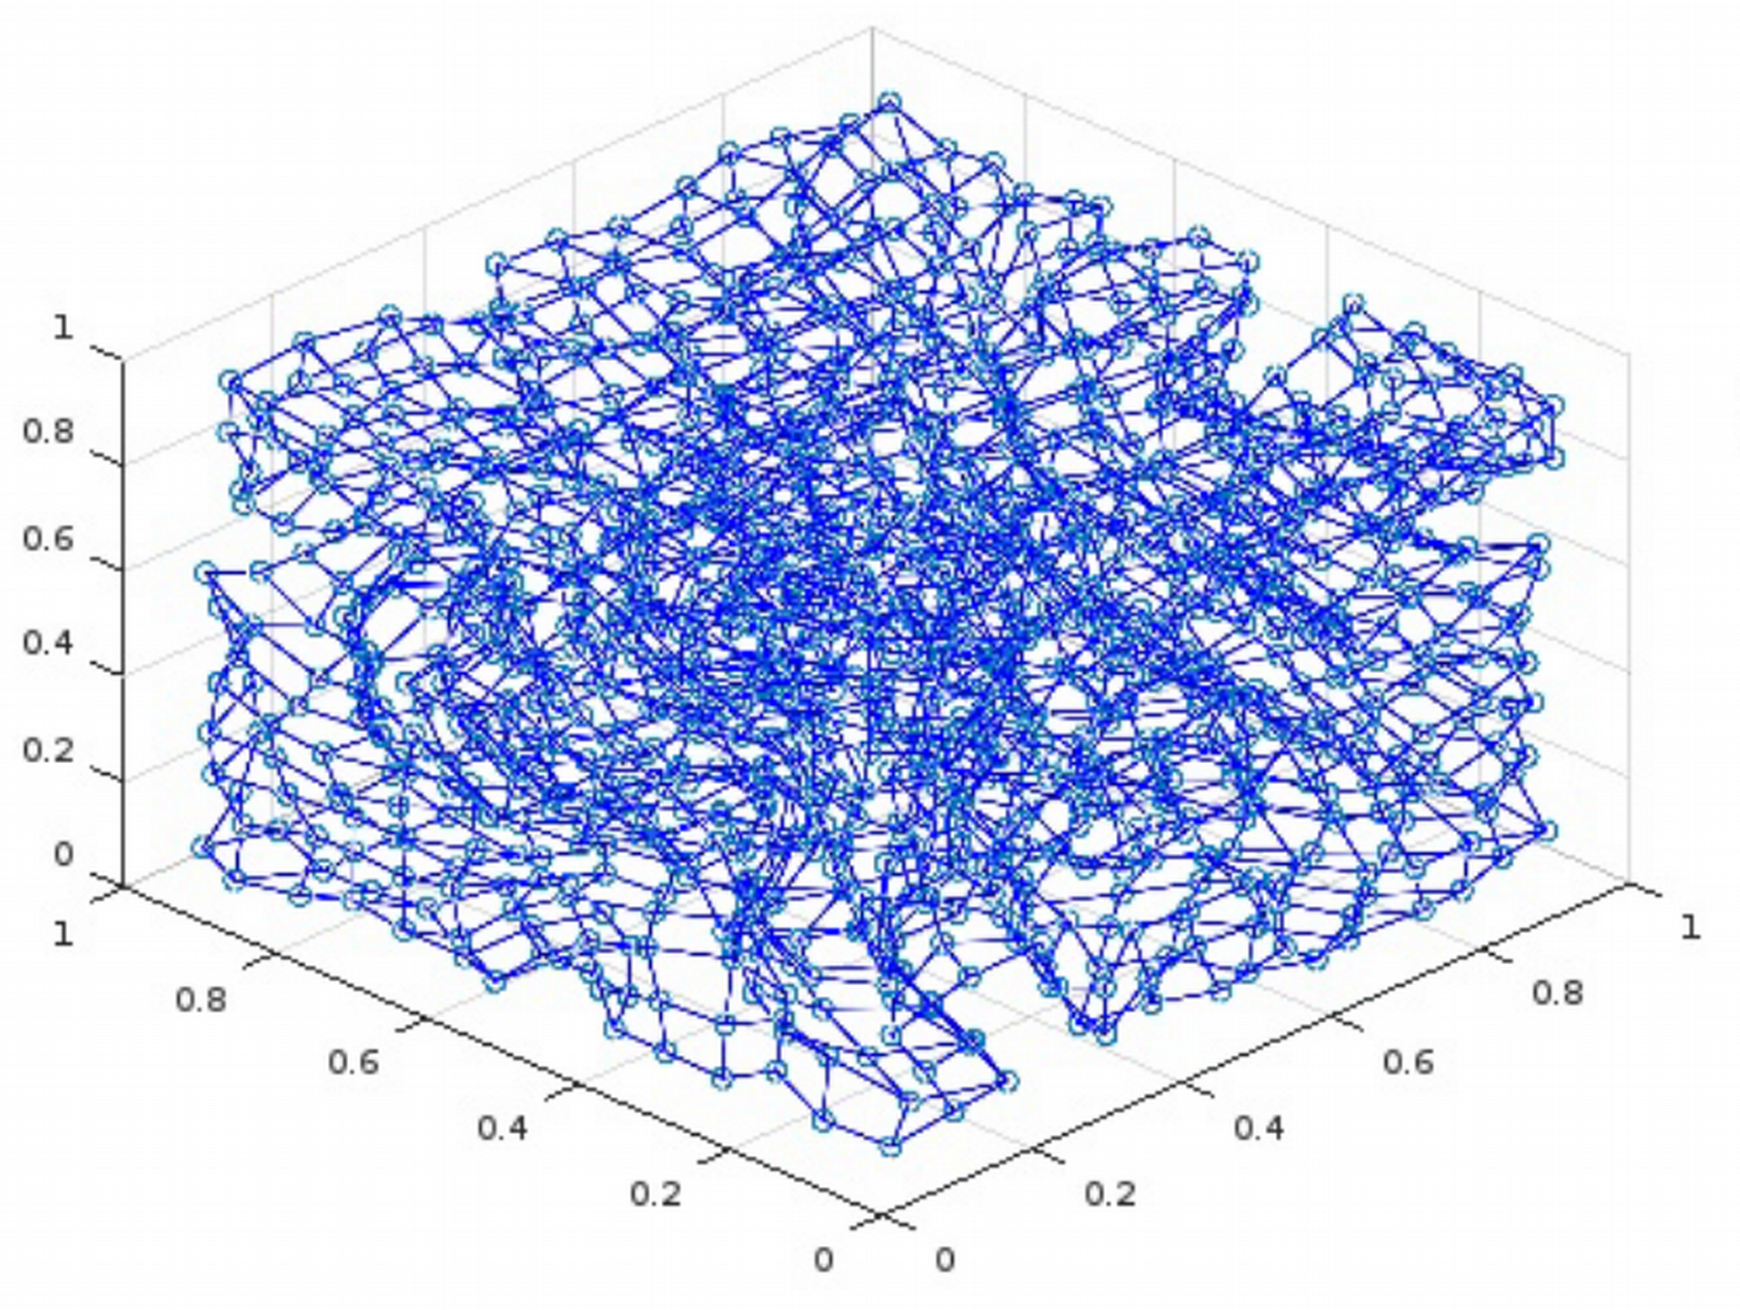
\includegraphics[width=0.4\textwidth]{SOM.png}
    %\caption{\glsfirst{som}. In the input, vectors are generated by a unit cube three-dimensional uniform distribution.
    %The array of neural units is a bi-dimensional lattice of 35 by 35 units which--by means of Alg. \ref{csom_proximal_synapses}--
    %tries to adapt to the input geometry in order to represent the input vectors as faithfully as possible.
    %The neural units are distributed in accordance with the statistical distribution in the input space.}
    %\label{fig:SOM}
%\end{figure}

%We call our implementation of the \gls{som} algorithm, \gls{ssom}. The \gls{ssom} algorithm accounts for proximal lateral intra-column interaction, \gls{ltp} and \gls{ltd}. It also dissociates proximal dendritic inputs from distal dendrites, since it modifies proximal connections following the statistical distribution from the \gls{mrstsa} independently of the units that fire in such \gls{cc}. This independence in the plasticity of the proximal dendritic inputs is supported by the property found in cortical tissue by means of which there is dendritic plasticity in the context of partial depolarization of the soma \cite{reiter_1998}--that is, without an \gls{ap}.

%The term \textit{static} comes from the fact that the patterns learned from proximal afferent dendrites do not account for the contextual history in the dynamic evolution of the algorithm.






%\subsection{\glsfirst{el} distal dendritic connections plasticity}
%\label{distal_dendrites}

%In terms of distal dendritic branches, each \gls{cc}--in this case we exemplify such \gls{cc} in red in Fig. \ref{fig:DistalDendrites}--in the \gls{el} is connected to other \glspl{cc}--in green in Fig \ref{fig:DistalDendrites}--by means of such branches inside the \gls{cc} receptive field--in yellow in Fig. \ref{fig:DistalDendrites}--from the same \gls{el} and from another \gls{cl} above. Each link between the red \gls{cc} and a green \gls{cc}--Fig. \ref{fig:DistalDendrites} A--symbolizes the fact that each cell unit in the red \gls{cc} is linked with a different subset of cell units in the green \gls{cc}--Fig. \ref{fig:DistalDendrites} B. Such subset of--random chosen--cells constitutes certain percentage from the total number of cells in the \gls{cc}. Such percentage is a tunable parameter for the model and determines the number of potential connections each cell in the red \gls{cc} has with respect to a green \gls{cc} in Fig. \ref{fig:DistalDendrites} B.

%\begin{figure}[h!]
    %\centering
    %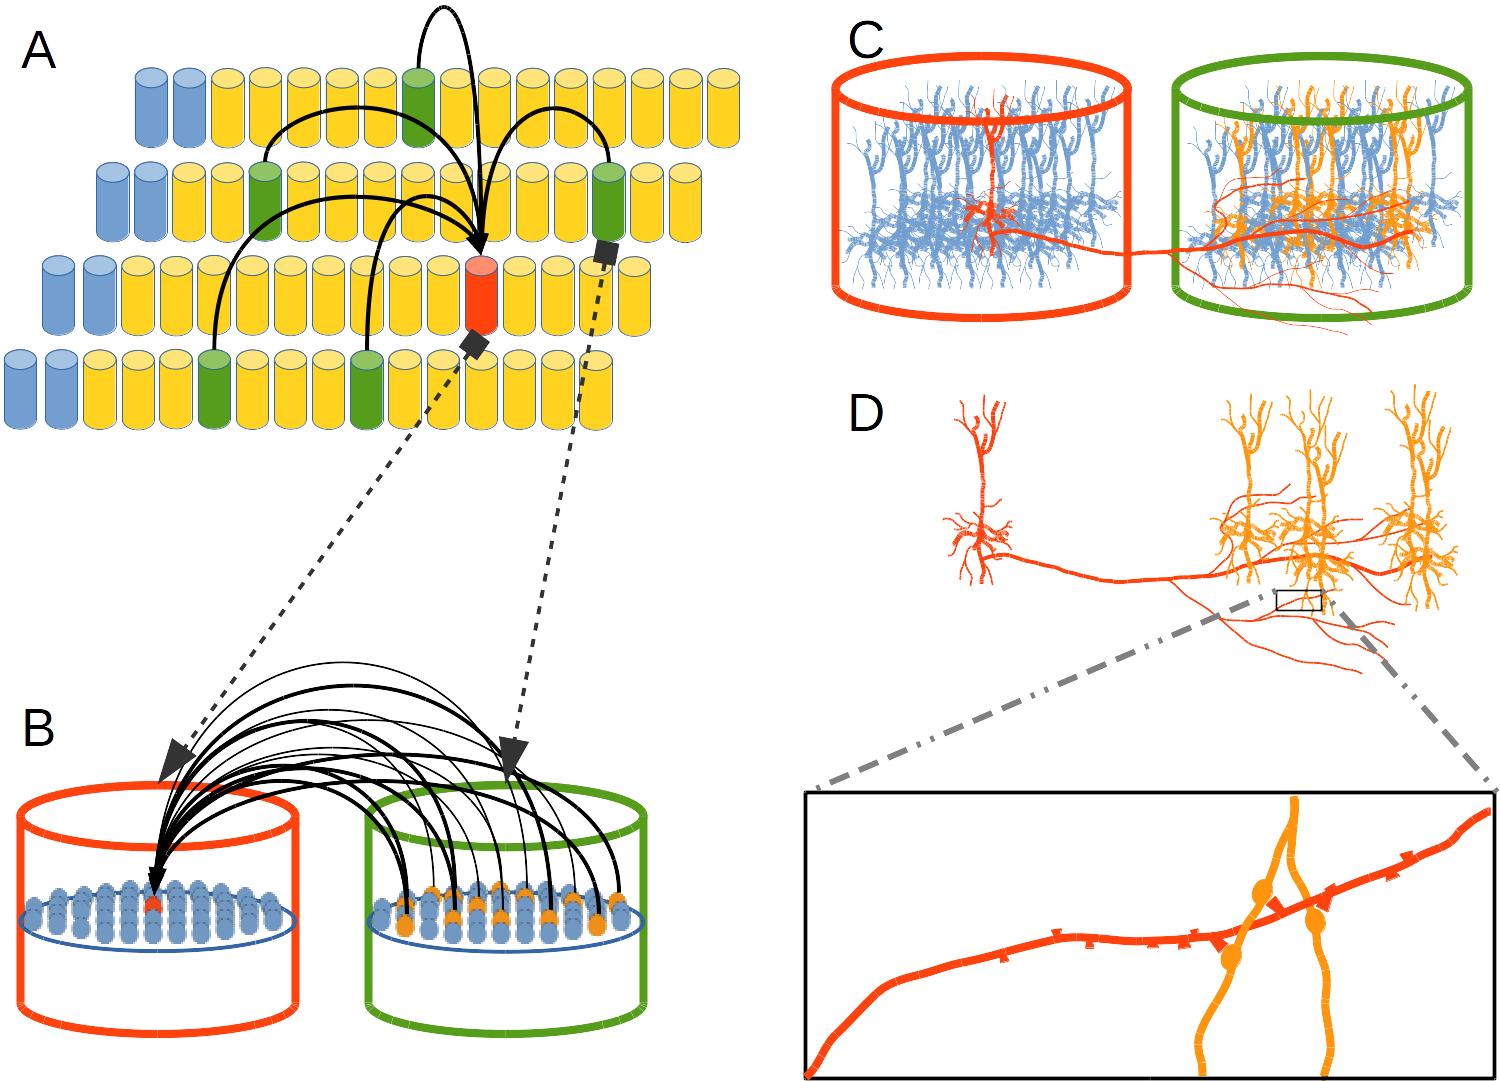
\includegraphics[width=0.7\textwidth]{DistalDendrites.png}
    %\caption{Distal dendrite connections. (A) Distal dendritic branches from neighboring \glspl{cc} inside the receptive field
    %of a \gls{cc} in the \gls{el}. A distal dendritic branch between the red \gls{cc} and a
    %green \gls{cc} means that every neural unit in the red \gls{cc} is linked with a different
    %subset of neural units in the green \gls{cc} by means of potential connections.
    %(B) Potential connections in a dendritic branch which link a neural unit in the red \gls{cc}
    %with a subset of neural units in a green \gls{cc}. The subset of potential connections comes from a percentage of neural units
    %inside the green \gls{cc}. Such percentage is a tunable parameter for the \gls{cc}.
    %(C) A distal dendritic branch between a pyramidal cell in a \gls{cc} and a 
    %sub-set of pyramidal cells in a neighboring \gls{cc} inside its receptive field
    %in the \gls{el}.
    %(D) Physical proximity of a dendritic branch from the red cell to axonal branches from yellow cells constitutes potential connections
    %which could prosper becoming in established synapses depending on the sequential activity among cells.}
    %\label{fig:DistalDendrites}
%\end{figure}

%Such links in Fig \ref{fig:DistalDendrites} A, represent dendritic branches in neural tissue and we call each connection in Fig. \ref{fig:DistalDendrites} B, potential connection. Potential connections represent synapses in the dendritic branch. A cell unit inside the red \gls{cc} ends up with as many dendritic branches as green \glspl{cc} inside its receptive field (Fig \ref{fig:DistalDendrites} A.)

%The term \emph{potential connection} is used, because it describes a pair of neural units linked by its physical location and dendritic and axonal disposition in cortical tissue (Fig. \ref{fig:DistalDendrites} C). However, an effective connectivity between such neurons will depend upon their sequential pattern of activation which will establish developed synapses between them. If two neural units--a red one and a yellow one in Fig. \ref{fig:DistalDendrites} D--are linked by means of a distal potential connection--produced by a synapse between a distal dendritic branch from the red one and an axonal branch from the yellow one--such connection will grow only if there is a sequential activation of the red cell after an activation of the yellow cell, in two consecutive time steps. If such phenomenon does not repeat itself over time, such synapse will decrease its strength with respect to other synapses in the dendritic branch in the red cell in Fig. \ref{fig:DistalDendrites} D. A simultaneous activation in both neural units--the red one and the yellow one in Fig. \ref{fig:DistalDendrites} D--will decrease the strength in such potential connection.

%We implemented distal dendritic synaptic plasticity mechanisms by means of an algorithm called \gls{dsom} (Alg. \ref{csom_distal_synapses}). The learning mechanisms implemented on such algorithm simulate neurophysiological phenomena such as \gls{stdp}, and homeostatic regulation plasticity in the synaptic strength regulation in distal dendritic branches.

%\begin{algorithm}
	%\caption{\texttt{Plasticity in Distal Synapses}. This algorithm plasticity and homeostatic phenomenon in distal dendritic synapses.}
%\label{csom_distal_synapses}
%\begin{algorithmic}[1]
	%\FOR{every active \texttt{unit} in this cortical \texttt{column}}
		%\FOR{every \texttt{dendrite} in this active \texttt{unit}}
			%\STATE {increment all the \texttt{synapses}--in this dendrite--potentially connected to \texttt{units} which were active in the last time step}
		%\ENDFOR
	%\ENDFOR
	%\FOR{every active \texttt{unit} in this cortical \texttt{column}}
		%\FOR{every \texttt{dendrite} in this active \texttt{unit}}
			%\STATE {decrement all the \texttt{synapses}--in this dendrite--potentially connected to \texttt{units} which are active in this time step}
		%\ENDFOR
	%\ENDFOR
	%\IF{updated \texttt{step} reaches certain value}
		%\FOR{every \texttt{unit} in this cortical \texttt{column}}
			%\FOR{every \texttt{dendrite} in this \texttt{unit}}
				%\IF{the sum of the \texttt{synapses} in this \texttt{dendrite} is greater than one}
					%\STATE {normalize all \texttt{synapses} in this \texttt{dendrite}}
				%\ENDIF
			%\ENDFOR
		%\ENDFOR
		%\STATE{updated \texttt{step} = 0}
	%\ENDIF
	%\STATE{updated \texttt{step}++} 
%\end{algorithmic}
%\end{algorithm}









%\subsection{\glsfirst{el} activation rules in a \gls{cc}}
%\label{activation_rules}

%In reference to the activation rules of neural units inside a \gls{cc} in the \gls{el},
%first a group of cell units in a \gls{cc} is partially depolarized 
%by distal connections among such neural units and cell units activated in the
%previous time step in the \gls{el}--Fig. \ref{fig:Activation} A.
%That is, neural units activated in time step $t=0$ in the \gls{el}, will partially depolarize
%a set of neural units in time step $t=1$ in such \gls{cc}, by means of distal--lateral and apical--
%dendritic branch synapses established by learning in the \gls{dsom} algorithm (Alg. \ref{csom_distal_synapses}).

%Second, afferent proximal connections from \gls{mrstsa} will tend to depolarize
%certain clusters of units in such \gls{cc} in time step $t=1$--Fig. \ref{fig:Activation} B.
%The tentative depolarization is produced by the inputs from the \gls{mrstsa} with
%proximal synapses established by learning in the \gls{ssom} algorithm (Alg. \ref{csom_proximal_synapses}). 
%Such group of neural units are randomly chosen from a discrete distribution
%whose probabilities are established by the state of excitation in afferent inputs.

%If a sufficient number of partially depolarized units are in the set of
%afferently excited units, such partially depolarized units
%will fire previously in the group--Fig. \ref{fig:Activation} B left.
%Those units--which fire before--prevent neighboring units in the excited clusters from firing,
%hyperpolarizing them by means of lateral inhibitory connections in the column.

%\begin{figure}[h!]
    %\centering
    %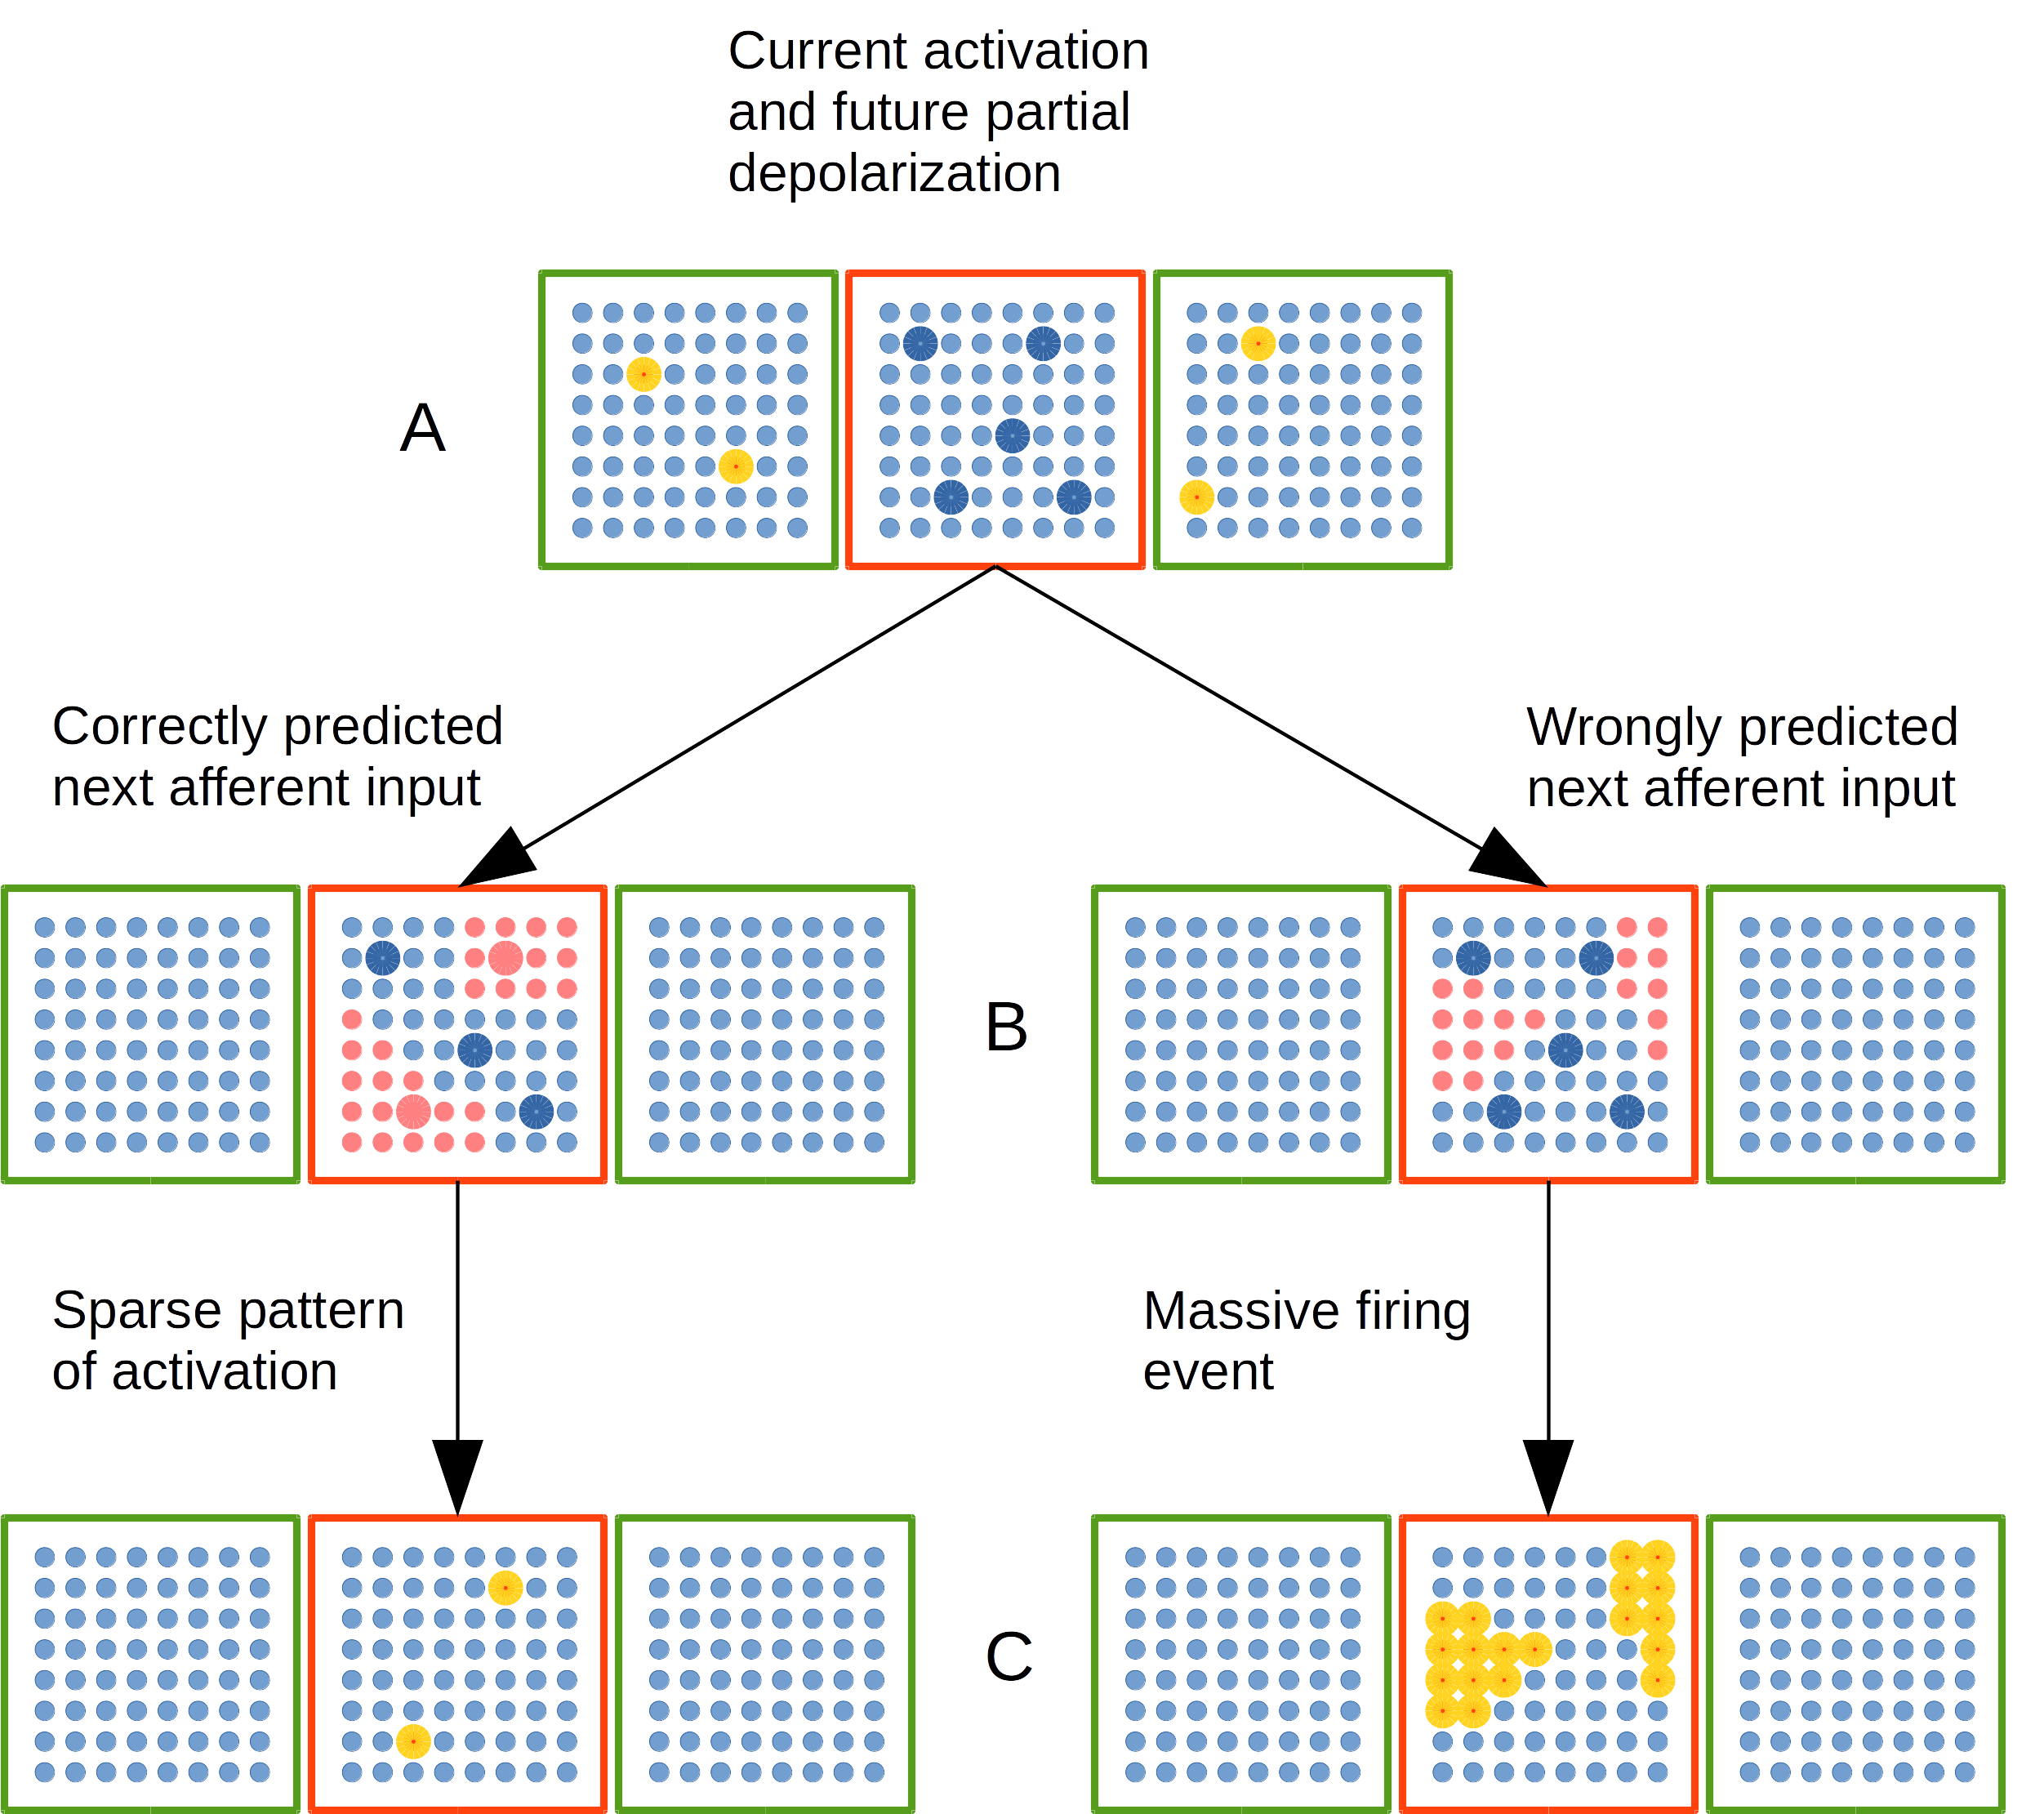
\includegraphics[width=0.7\textwidth]{Activation.png}
    %\caption{Dynamic cellular activation in a \gls{cc} in the \gls{el}.
    %A red cortical column is linked with two green cortical columns by means of distal dendrites.
    %(A) Cellular activation in green \glspl{cc}--highlighted yellow cells--puts neural units
    %in red \gls{cc} in a partially depolarized--predictive state highlighted in blue.
    %(B) Cluster of neural cells activated by afferent inputs.
    %Left: A substantial amount of partially depolarized cells are in the afferently excited cellular clusters.
    %Right: There is no substantial amount of partially depolarized cells inside afferently excited cellular clusters.
    %(C) \gls{cc} with active cellular units highlighted in yellow.
    %Left: Sparse pattern of cellular activation.
    %Right: Massive pattern of activation.}
    %\label{fig:Activation}
%\end{figure}

%Partial depolarization states put cell units in a predictive state generated by
%the activations produced in the \gls{el} in previous time steps.
%That is, lateral and apical activation in previous time steps constitutes a context in which
%current afferent inputs are received.

%From the group of units that tend to be depolarized by current afferent inputs from the \gls{mrstsa},
%only a reduced sub-set of those units are likely to fire in the previous contextual firing history
%in the \gls{el}--Fig. \ref{fig:Activation} C left.

%In case there is no context, that is, not enough number of the units which tend to be depolarized by afferent inputs
%is partially depolarized by previous--lateral and apical--activations--Fig. \ref{fig:Activation} B right--,
%all units in the afferent excited clusters will be active, covering more hypotheses for next inputs--Fig. \ref{fig:Activation} C right.

%Such activation mechanism is depicted in Alg. \ref{csom_activation}. In Alg. \ref{csom_activation} (Part 1) a ranking is established between neural units--inside a \gls{cc}--in terms of its afferent excitability, given the afferent inputs (lines 1 and 2). The \emph{number of afferently excited units} makes reference to the maximum number of  units that can be activated by the afferent input in a \gls{cc} and \emph{minimum number of active units} makes reference to the number of units that will be active in a \gls{cc} if a \gls{sdr} is achieved as a result of optimal prediction (lines 3 and 4 respectively).

%\begin{algorithm}
	%\caption{\texttt{Units activation (Part 1)}. This algorithm establishes the activation rules in a \gls{csom} object.}
%\label{csom_activation}
%\begin{algorithmic}[1]
	%\STATE{\texttt{distances} = given an \texttt{input} vector find the euclidean distance each \texttt{unit} has to such \texttt{input} in the input space from proximal afferent synapses}

	%\STATE {\texttt{ranking} = sort indexes from the smallest to the largest \texttt{distances}}

	%\STATE{number of afferently excited units = proximal activation percentage*number of units}

	%\STATE{minimum number of active units = (1-sparsity)*number of units}

	%\IF{randomness is disabled}
		%\STATE {excited \texttt{units} = gets the first \emph{number of afferently excited units} elements from \texttt{ranking}}
	%\ELSE
		%\STATE {excited \texttt{units} = gets \emph{number of afferently excited units} random indexes from \texttt{distances} with probabilities determined by the relative reciprocal of the \texttt{distances} element values}
	%\ENDIF

	%\FOR{\texttt{unit} = 0 \TO \texttt{unit} = number of units }
		%\STATE{auxiliary = 0}
		%\FOR{\texttt{dendrite} = 0 \TO \texttt{dendrite} = number of distal dendrites }
			%\STATE{\texttt{dendrite} accumulator = 0}
			%\FOR{\texttt{active unit} = 0 \TO \texttt{active unit} = number of linked active units}
				%\STATE{potential \texttt{index} = find the first coincident index in potential \texttt{connections[dendrite][unit]} with linking \texttt{units[dendrite][active unit]}}
				%\IF{there exist coincidence}
					%\STATE {\texttt{dendrite} accumulator += dynamic \texttt{synapses[dendrite][unit][\textnormal{potential} index]}}
				%\ENDIF
			%\ENDFOR
			%\IF{\texttt{dendrite} accumulator > 100*DISTAL\_SYNAPTIC\_THRESHOLD}
				%\STATE {auxiliary++}
			%\ENDIF
		%\ENDFOR
		%\STATE{total \texttt{responses[unit]} += auxiliary}
	%\ENDFOR
	%\STATE{updated \texttt{distances} = element wise quotient between \texttt{distances} and total \texttt{responses}}
	%\STATE {updated \texttt{ranking} = sort indexes from the smallest to the largest updated \texttt{distances}}

%\end{algorithmic}
%\end{algorithm}

%If randomness is enabled, \emph{number of afferently excited units} amount of units is chosen at random by means of a discrete distribution whose probabilities are the afferent excitation of each unit. If randomness is disabled, \emph{number of afferently excited units} first units are chosen from the ranking of afferently excited units (lines 5 to 9). 

%From line 10 to 25 each neural unit accumulates distal--lateral and apical--excitation in order to determine its partial depolarization from units which were active in the previous time step. For each neural unit in a \gls{cc}, for each distal dendrite in such unit and for each active unit in such distal dendrite the algorithm looks for coincidences between some potential connection in such distal dendrite in the neural unit and the active active unit in such distal dendrite. That is, in line 15, the algorithm ask if there is coincidence between some potential connection in this distal dendrite inside the unit and the neural unit activated in the previous time step in the \gls{cc} linked by such distal dendrite. If there is coincidence, the value of the synaptic weight in such potential connection is accumulated in a dendrite accumulator. After all active units are examined for this dendrite, if the dendrite accumulator is greater than certain threshold, such dendrite is considered active and the total response of the unit is incremented in one.

%Each neural unit ends up with an excitation value due to its distal dendrites. The unit distances vector is element wise divided by distal dendritic excitations vector to get the updated distances and an updated ranking of the units (lines 26 and 27). In this way, units with more distal excitation will decrease its distance more and will be put in a more favorable place in the ranking in order to be activated.

%In Alg. \ref{csom_activation} (Part 2) the minimum updated distance is found in the group of afferently excited units. Then, a set of units--inside the group of afferently excited units--is identified which have such minimum updated distance. While the number of identified units is less than \emph{minimum number of active units}, the next   minimum updated distance is found in the group of afferently excited units and a new set of units--inside the group of afferently excited units--is identified which have such next minimum updated distance. This new set is added to the previous one until the number of units in this accumulative set is greater than or equal to the minimum number of active units.

%\begin{algorithm}
%\ContinuedFloat
%\caption{\texttt{Units activation (Part 2)}. This algorithm establishes the activation rules in a \gls{csom} object.}
%\label{csom_activation}
%\begin{algorithmic}[1]
	%\STATE{new \texttt{distances} = get the updated \texttt{distances} elements whose indexes are in excited \texttt{units}}
	%\STATE{new minimum \texttt{distance} = get the minimum element from new \texttt{distances}}
	%\STATE{minimum \texttt{indexes} = get indexes from updated \texttt{distances} vector whose values are equal to new minimum \texttt{distance}}
	%\STATE{apt to be \texttt{active} = get the coincident indexes between excited \texttt{units} and minimum \texttt{indexes}}
	%\STATE{erase from new \texttt{distances} vector, all the elements whose value is equal to new minimum \texttt{distance}}

	%\WHILE{number of elements in apt to be \texttt{active} vector < \emph{minimum number of active units} and new \texttt{distances} has at least one element}
		%\STATE{new minimum \texttt{distance} = get the minimum element from new \texttt{distances}}
		%\STATE{minimum \texttt{indexes} = get indexes from updated \texttt{distances} vector whose values are equal to new minimum \texttt{distances}}
		%\STATE{partial apt to be \texttt{active} = get the coincident indexes between excited \texttt{units} and minimum \texttt{indexes}}
		%\STATE{incorporate partial apt to be \texttt{active} elements into apt to be \texttt{active} vector}
		%\STATE{erase from new \texttt{distances} vector, all the elements whose value is equal to new minimum \texttt{distance}}
	%\ENDWHILE

	%\IF{ENABLE\_RANDOM\_BEHAVIOUR}
		%\STATE {shuffle apt to be \texttt{active} vector}
	%\ENDIF

	%\FOR{\texttt{number} = 0 \TO \texttt{number} = number of apt to be \texttt{active} elements }
		%\STATE {incorporate to \texttt{output} the excited \texttt{units[\textnormal{apt to be} active[number]]}}
	%\ENDFOR

	%\RETURN \texttt{output}
%\end{algorithmic}
%\end{algorithm}

%The functional result of Alg. \ref{csom_activation} is that there must be a sufficient amount of--partially and previously depolarized-- neural units inside the afferently activated cluster of units in order to get a \gls{sdr} pattern of activation. Otherwise, the \gls{cc} will end up with a massive activation pattern \gls{mfe} in which more than a \emph{minimum number of active units} will be active. In the case of the occurrence of a \gls{mfe}, the synaptic plasticity is modulated in order to form stronger synapses of those neural units activated during such event. 

%Each neural unit in a \gls{cc} establishes its state of partial depolarization based on the contribution from distal dendritic branches from lateral and apical connections. A dendritic branch will contribute to the partial depolarization of the soma in such cell only if such dendritic branch exceeds an activation threshold by means of the contribution from its individual synapses in the context of the patterns of activation in the previous time step.

%This mechanism has compelling sequential properties \cite{hawkins_2016}, which have already been applied in the classification of artificially generated sequential data \cite{cui_2016}. We apply such mechanism in the \gls{dsom} algorithm by adding the contribution of synapses--in a dendritic branch--whose connections are linked with cells that were active in the previous time step in the \gls{el}.











%\subsection{\glsfirst{el} Class}

%The \gls{el} is a multidimensional array of \glspl{cc} that obtains \glspl{sdr} from proximal afferent connections from the \gls{mrstsa}, from distal lateral connections from the same \gls{el} and from distal apical connections from other \gls{cl} above the \gls{el}. In Fig. \ref{fig:EncoderColumnConnections} we exemplify the connectivity profile of a \gls{cc}--in red--inside the \gls{el} which is a bi-dimensional array of \glspl{cc}. Such red \gls{cc} has an afferent receptive field on the \gls{mrstsa}, a lateral receptive field on the same \gls{el} and an apical receptive field on another \gls{cl} above the \gls{el}. Receptive fields are highlighted in yellow in Fig. \ref{fig:EncoderColumnConnections}. The position of the red \gls{cc} above the \gls{mrstsa} and below the other \gls{cl} in Fig. \ref{fig:EncoderColumnConnections} determines its corresponding centers on the \gls{mrstsa} array and on the \gls{cl} above the \gls{el}. Each receptive field has a size which is developed about its \gls{cc} corresponding centers. In the case depicted in Fig. \ref{fig:EncoderColumnConnections} receptive fields have wraparound property. This property allows receptive fields to extend beyond the physical limits imposed by sides and/or corners, using space on opposite sides and corners in the layers. Wraparound property as well as size of the receptive fields are tunable parameters in the \gls{el}. If wraparound property is disabled, \glspl{cc} centers near sides and corners in the layer will receive less receptive field surface. \gls{cc} receptive fields determine the connectivity scope of such \gls{cc} in the different layers of the model. Inside each receptive field, there are some green modules in Fig. \ref{fig:EncoderColumnConnections} which represent elements which are really connected to the red \gls{cc} in such receptive fields. Each set of green elements constitutes certain percentage from the total number of elements in its corresponding receptive field. Such percentage is also a tunable parameter in the \gls{el}. 

%\begin{figure}[h!]
    %\centering
    %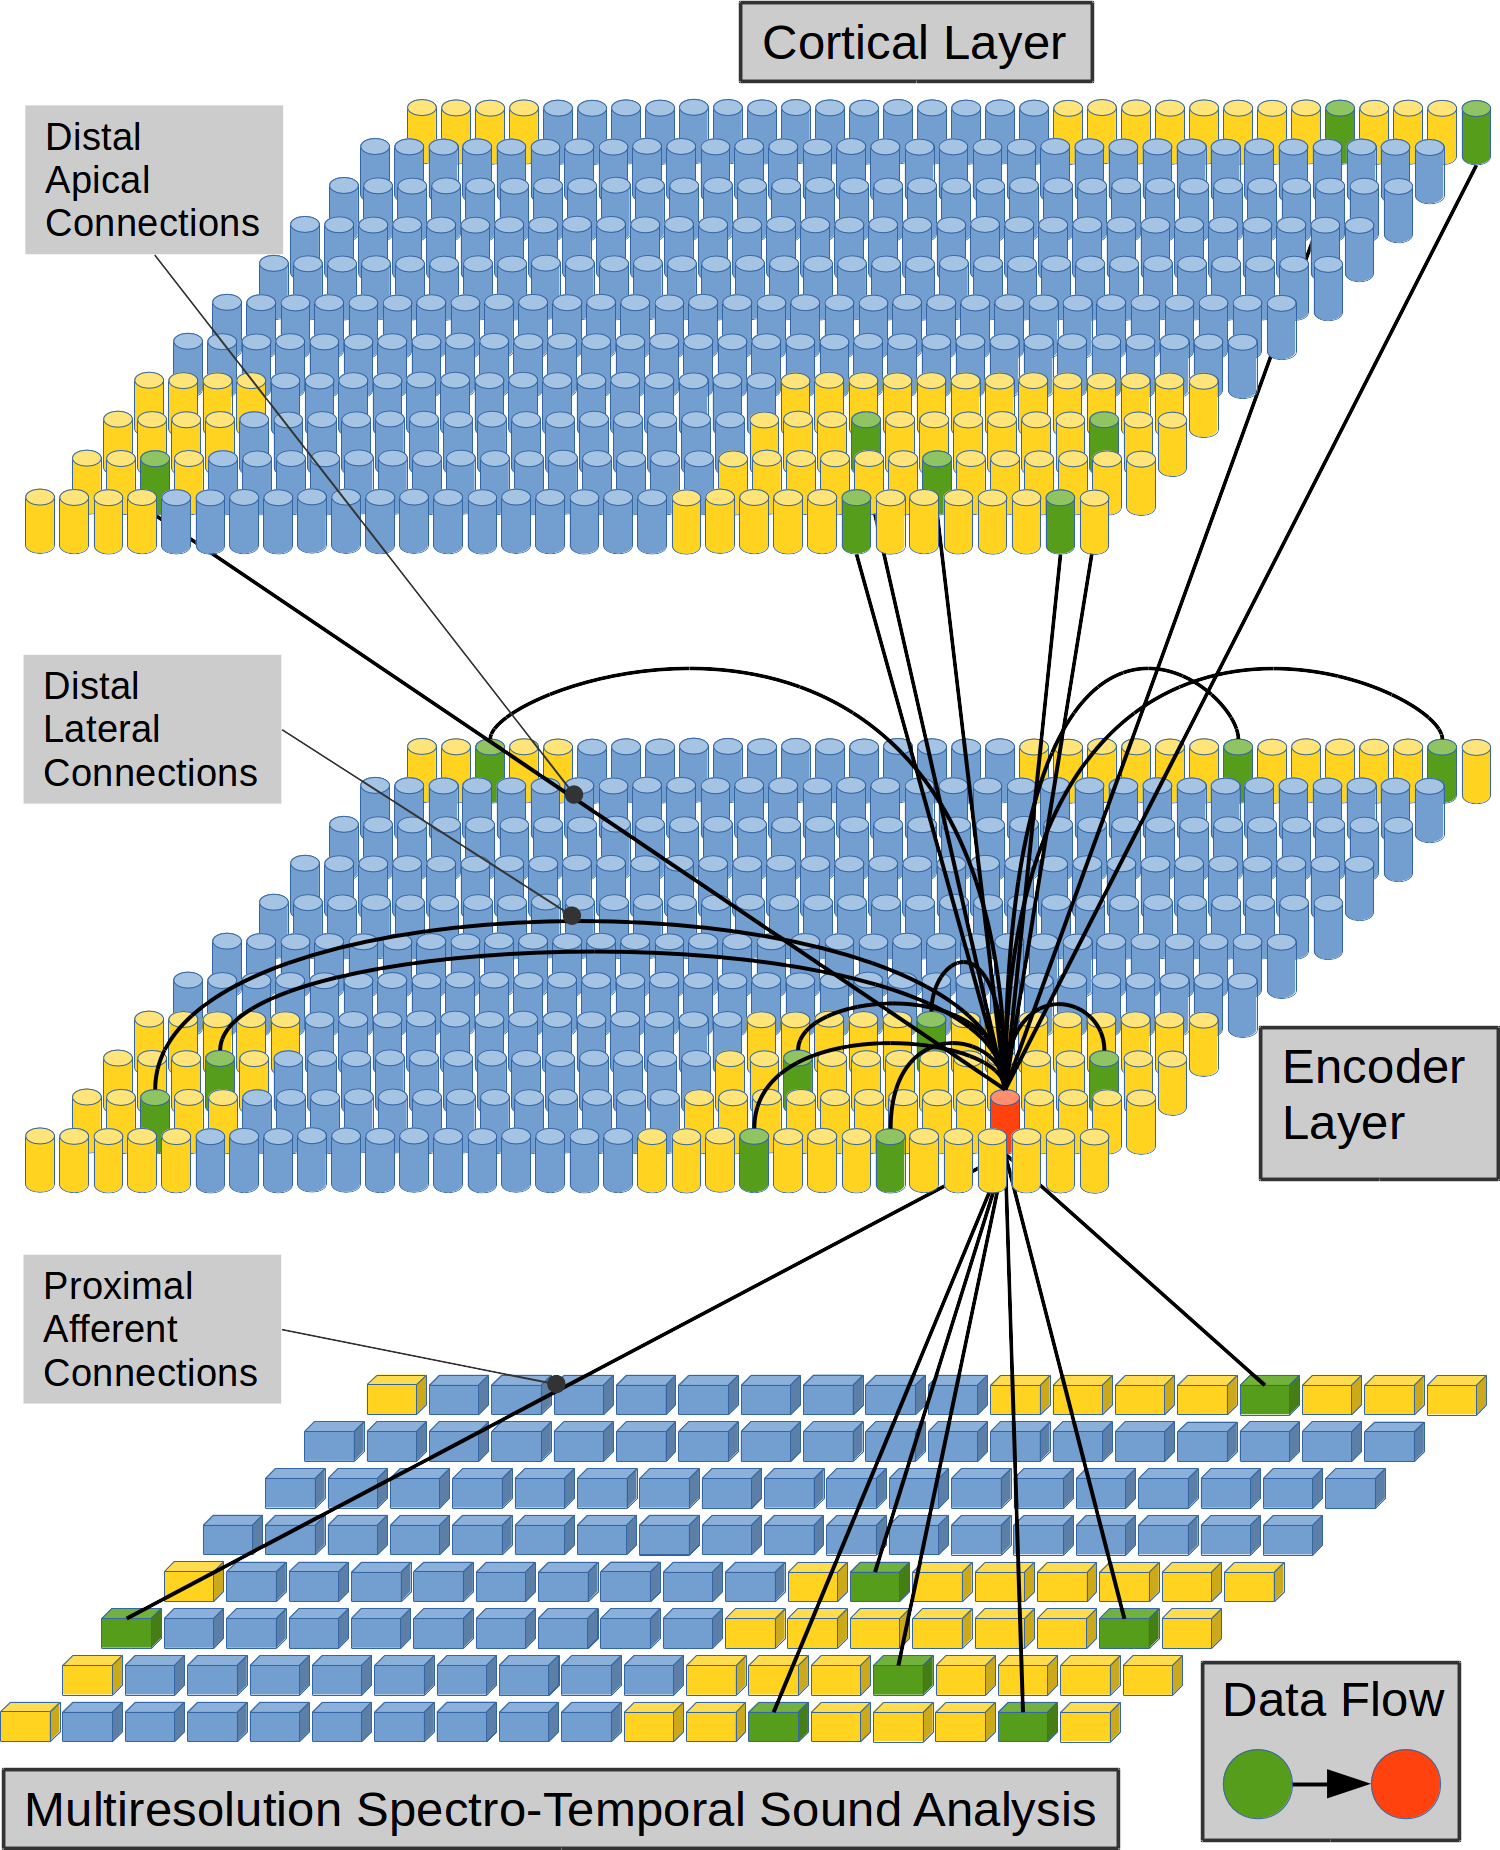
\includegraphics[width=0.6\textwidth]{EncoderColumnConnections.png}
    %\caption{Connection scheme for a cortical column in the Encoder Layer.
    %Each cylinder in the \gls{el} and in the \gls{cl} represents a \gls{cc} in neural tissue.
    %Each prism in the \gls{mrstsa} represents a real valued variable.
    %This is a visualization of a \gls{cc} (in red) and its three receptive fields (in yellow).
    %The receptive field of a \gls{cc} is an array that defines a set of \glspl{cc}
    %with which such column could be connected.
    %The receptive field of a \gls{cc} on the \gls{mrstsa} determines an array of real valued variables
    %with which such column could be connected.
    %A subset of \glspl{cc} in a receptive field (in green) represents the \glspl{cc} that are really
    %connected with the \gls{cc} in red. A similar scenario could be described for the green prisms on
    %the \gls{mrstsa}.
    %The size, wrap-around property and percentage of established links (in green) inside a receptive field are tunable parameters for the model.
    %In this work, only lateral connections have been implemented since in the current implementation there are no upper cortical layers from which
    %to bring apical connections.}
    %\label{fig:EncoderColumnConnections}
%\end{figure}

%Individual modules on the \gls{mrstsa} are very different from individual modules on the \gls{el} or on the \gls{cl} above. Individual modules on the \gls{mrstsa} are scalar--real valued--variables (section \ref{mrstsa}) while individual modules on the \gls{el} and \gls{cl} are \glspl{cc}. This circumstance determines that proximal afferent connections are very different from distal--lateral and/or apical--connections. While proximal afferent connections are individual synaptic weights (section \ref{proximal_dendrites}), distal connections are complex dendritic branches (section \ref{distal_dendrites}). 

%The \gls{el} class configures all the connectivity for each \gls{cc}, that is, determines the random elements from the \gls{mrstsa}--inside the receptive field of such \gls{cc}--which will be linked with the \gls{cc}, determines the random set of potential connections to each element in each distal dendrite. All this connectivity configurations for each \gls{cc} is saved after an initial procedure of construction of a \gls{el} object. 

%In each time step, the \gls{el} gathers the information from afferent, lateral and apical connections and makes this information available for each \gls{cc}. In the \gls{som} algorithm, each input vector has to be completely determined. In our case, some inputs from the \gls{mrstsa} could be null, and each input vector could not have the information of each of its components available. We incorporated a stochastic mechanism in the \gls{el} in order to deal with such situation. We made each afferent connection to learn statistical boundaries from its corresponding input. We establish a minimum-maximum margin in each proximal connection in the \gls{el}. Such margin is consistent with the statistical distribution in the history of its corresponding input. When an afferent input is undetermined, in a context in which some afferent inputs have available information, the \gls{el} chooses the value in the undetermined input randomly between the boundaries learned for such input.












\section{Computational Implementation}

\subsection{\glsfirst{el} Implementation}

\subsubsection{\glsfirst{el} Hierarchical Inheritance and Compositional Structure}

We implemented our algorithms in the standard \CC14 using the \gls{oop} paradigm in a set of classes interrelated by inheritance and composition. We configured the~\gls{el} class as a composition of objects of class \glsfirst{csom}. The main member in the \gls{el} class is a \gls{stl} vector of \gls{csom} objects. Each \gls{csom} object in the \gls{stl} vector represents a \gls{cc} in the \gls{el}. A complete diagram of the hierarchical inheritance and compositional structure of the implementation can be seen in Fig. \ref{fig:InheritanceComposition}.

%We implemented our algorithms in standard \CC14 using the \gls{oop} paradigm in a set of classes interrelated by inheritance and composition. We implemented proximal afferent and distal inter-columnar connectivity as well as minimum-maximum margins in afferent synaptic weights in the \glsfirst{el} class. We configured such class as a composition of objects of class \glsfirst{csom}. The main member in the \gls{el} class is a \gls{stl} vector of \gls{csom} objects. Each \gls{csom} object in the \gls{stl} vector, represents a \gls{cc} in the \gls{el}. A complete diagram of the hierarchical inheritance and compositional structure of the implementation can be seen in Fig. \ref{fig:InheritanceComposition}.

\begin{figure}[h!]
    \centering
    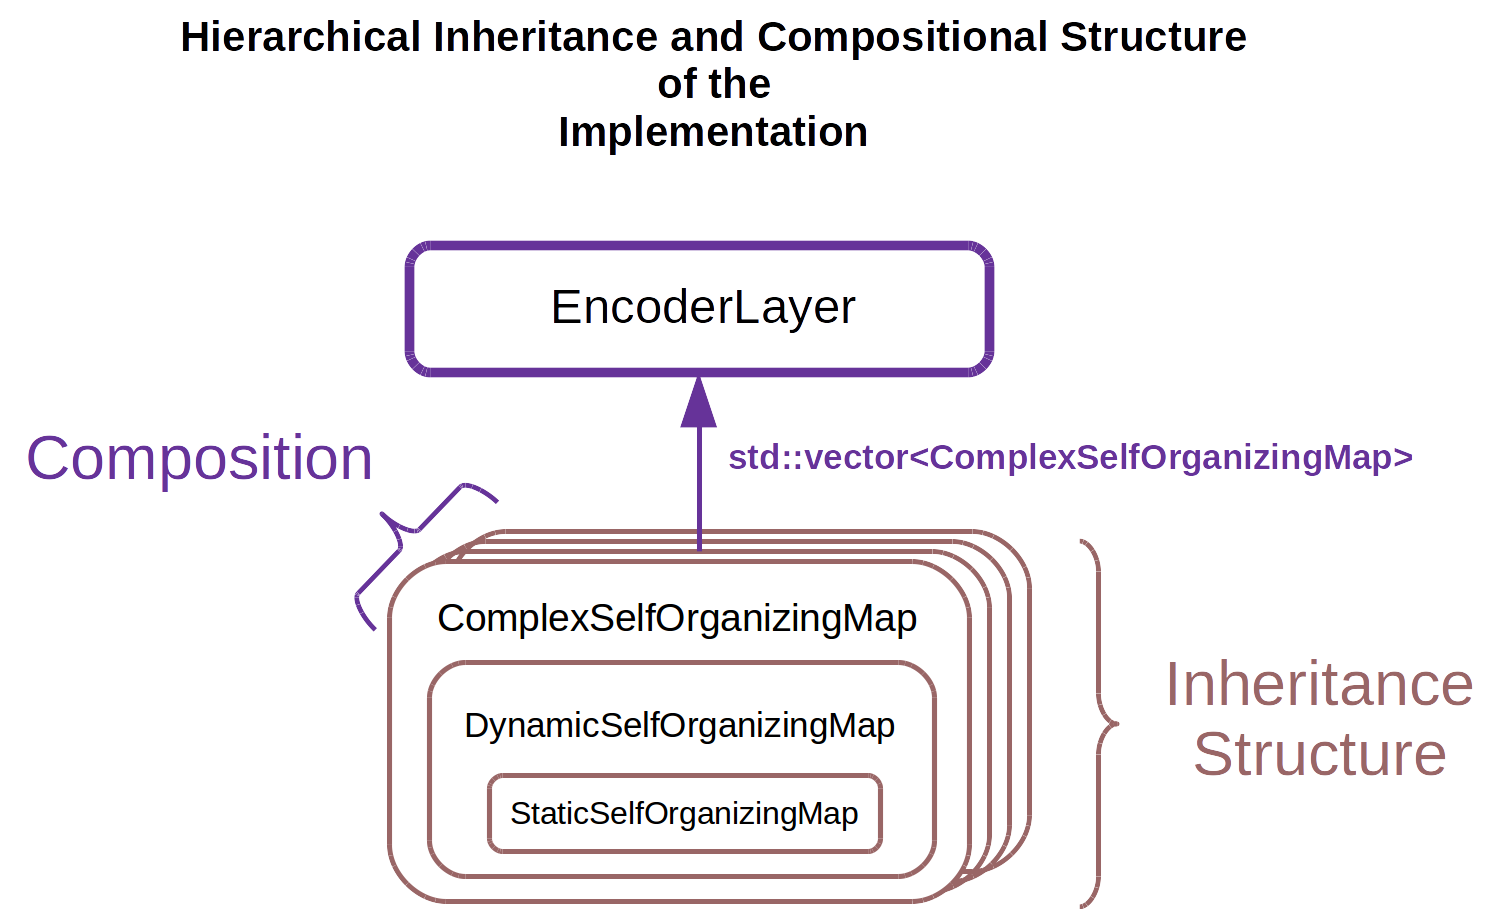
\includegraphics[width=0.6\textwidth]{InheritanceComposition.png}
    \caption{Hierarchical Inheritance and Compositional Structure of the \gls{el}. \glsfirst{csom} inherits from \glsfirst{dsom} which inherits from \glsfirst{ssom}. The \glsfirst{el} is composed by a set of \glspl{csom} gathered    in a std::vector \glsfirst{stl} container.}
    \label{fig:InheritanceComposition}
\end{figure}

The \glsfirst{ssom} class implements proximal connections, the \glsfirst{dsom} class implements distal connections and the \glsfirst{csom} class implements activation rules in a~\gls{cc}. Each class uses \gls{stl} vectors to store its data and \texttt{algorithm} \gls{stl} library to computationally operate through iterators or pointers on those vectors.

%The \glsfirst{ssom} class implements Alg. \ref{csom_proximal_synapses} explained in section \ref{proximal_dendrites}, the \glsfirst{dsom} class implements Alg. \ref{csom_distal_synapses} explained in section \ref{distal_dendrites} and the \glsfirst{csom} class implements Alg. \ref{csom_activation} explained in section \ref{activation_rules}. Each class uses \gls{stl} vectors to store its data and \texttt{algorithm} \gls{stl} library to computationally operate through iterators or pointers on those vectors.






























\subsubsection{\glsfirst{el} Parallelization}

We parallelized the \gls{el} class by means of a hybrid \gls{mpi}+\gls{omp} paradigm. We distributed \glspl{csom} among \gls{mpi} ranks as a deck of cards is distributed among different players. Each \gls{mpi} rank ends up with one or more \glspl{csom} and the \glspl{csom} in each rank are distributed among different \gls{omp} threads (Fig. \ref{fig:EncoderParallelization} A and B respectively and Alg.~\ref{ccs_distribution}).

\begin{algorithm}
	\caption{This algorithm distributes \glspl{cc} among \gls{mpi} processes in a distributed memory system and the \glspl{cc} in each process are distributed among \gls{omp} threads in a shared memory system. In this algorithm we run one \gls{mpi} process per compute node on Cooley.}
\label{ccs_distribution}
\begin{algorithmic}[1]
	\STATE {\texttt{numberOfProcesses} = getNumberOfProcesses()}
	\STATE {\texttt{processNumber} = getProcessNumber()}
	\STATE {\#\textbf{pragma omp parallel for} default(none) shared(\texttt{processNumber}, \texttt{numberOfProcesses})}
	\FOR{\texttt{column} = \texttt{processNumber} \TO \texttt{column} = number of \glspl{cc}; \texttt{column} += \texttt{numberOfProcesses}}
	\STATE {Do \gls{csom} stuff...}
	\ENDFOR
\end{algorithmic}
\end{algorithm}

\begin{figure}[h!]
    \centering
    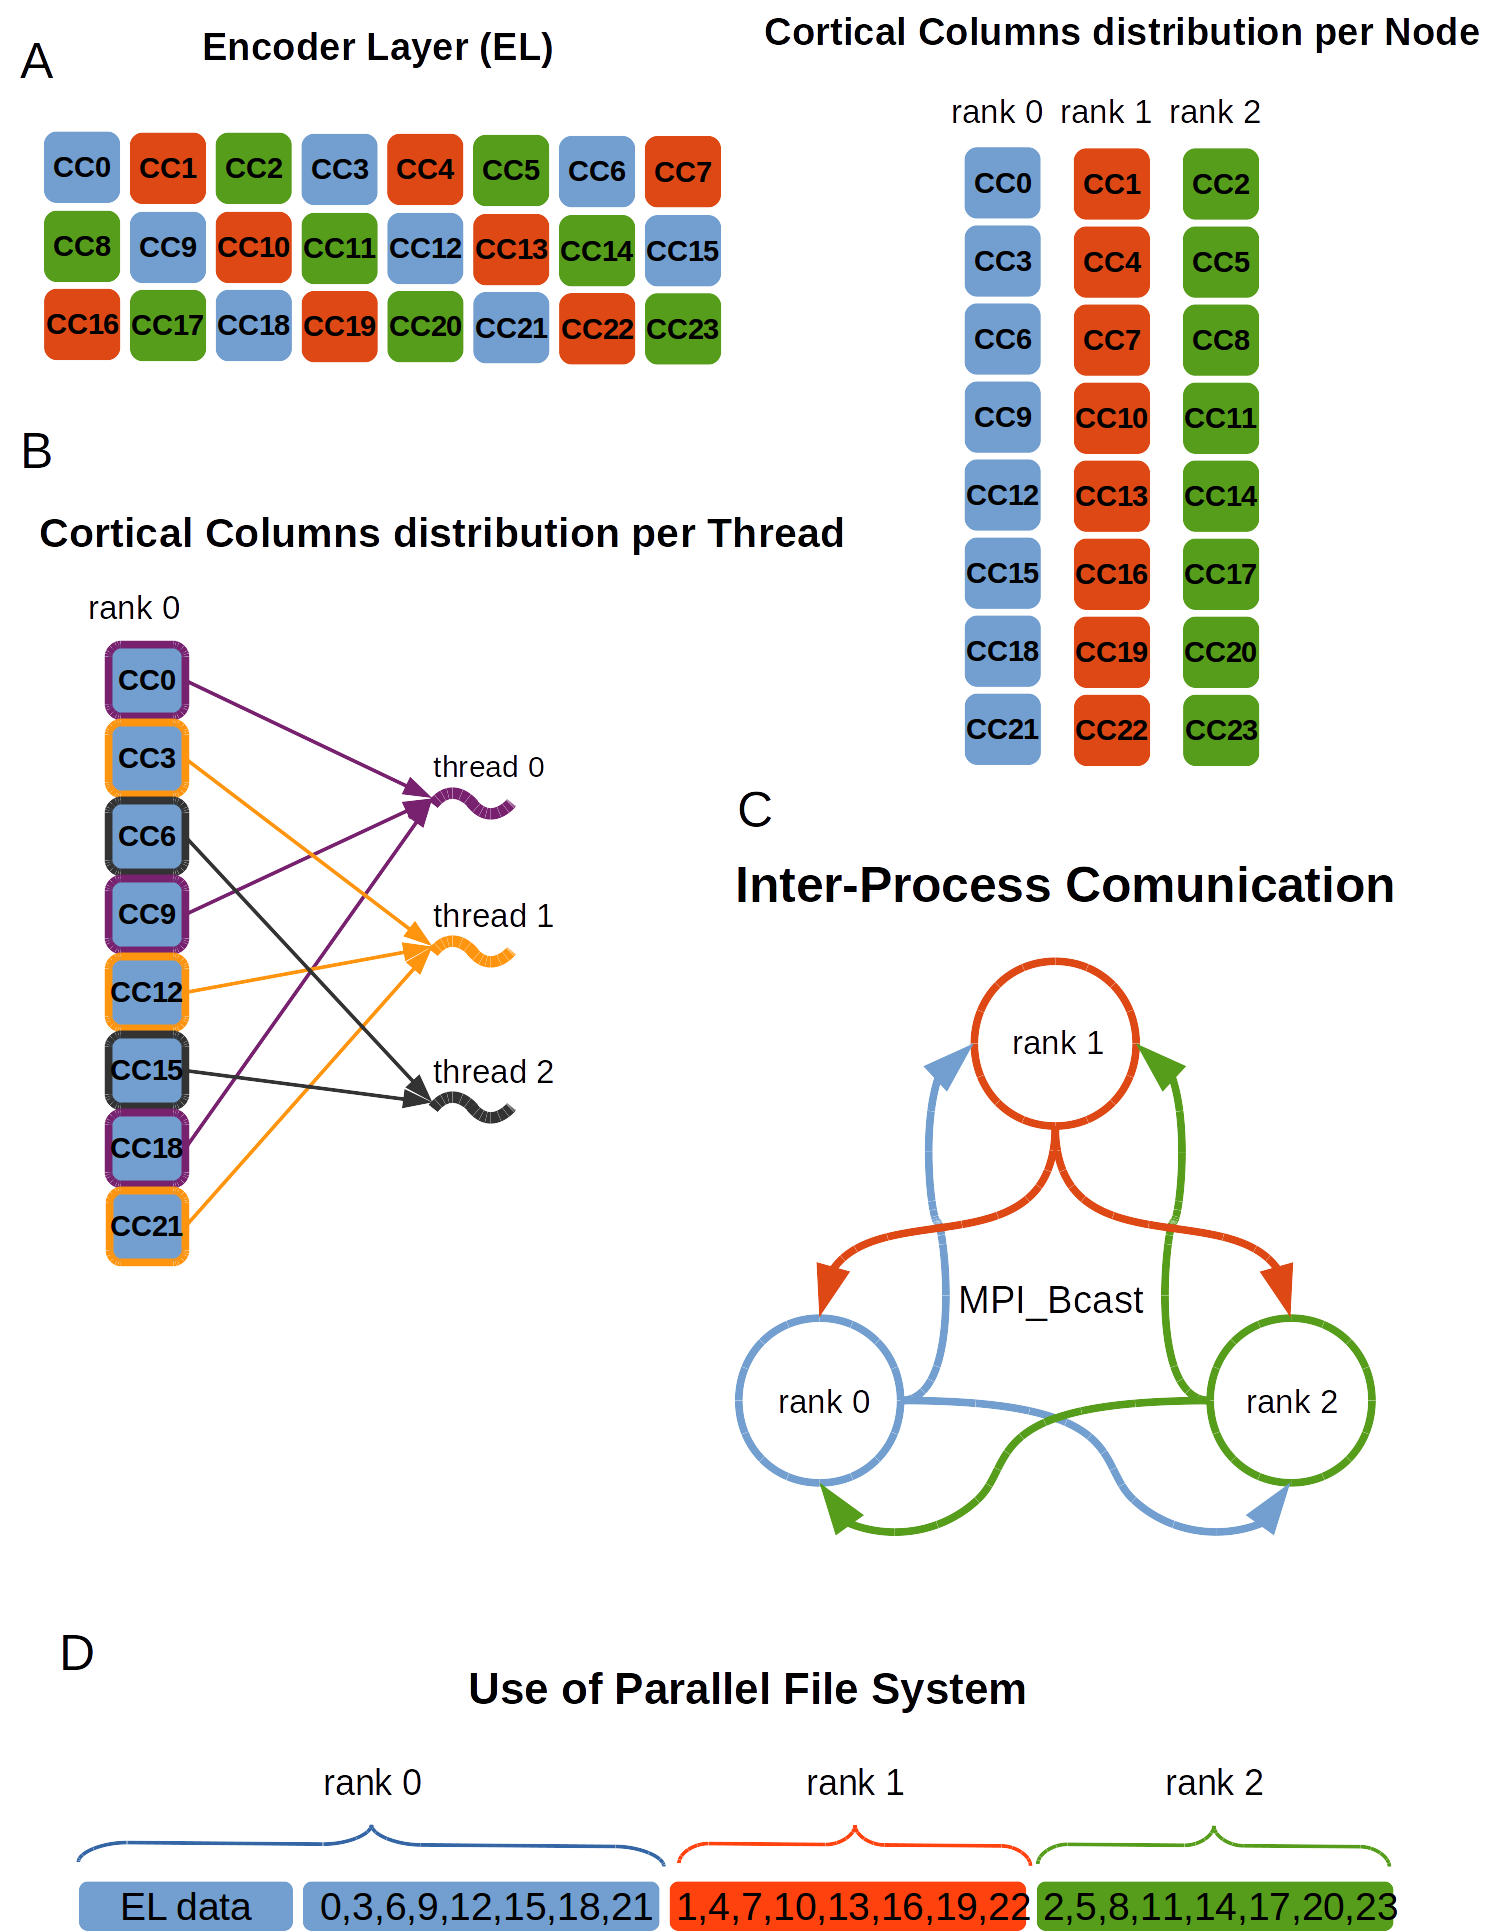
\includegraphics[width=0.5\textwidth]{EncoderParallelization.png}
    \caption{\glsfirst{el} \gls{mpi}+\gls{omp} parallelization. (A) Distribution of \gls{csom} objects in an \gls{el} with
    3 by 8 (24) \glspl{cc} among three \gls{mpi} ranks with three \gls{omp} threads per rank.
    Certain ranks could take care of a different number of
    \glspl{csom} depending on the number of \gls{mpi} ranks as well as the number of \glspl{cc} in the \gls{el}.
    (B) Each \gls{mpi} rank distributes its \glspl{csom} among different threads in the same fashion.
    (C) \gls{mpi} \gls{ipc} among different ranks. \gls{ipc} is carried out at each time step since each \gls{mpi} rank 
    requires the complete \gls{el} output at each time step.
    Each \gls{mpi} rank broadcasts the information corresponding to its \glspl{cc} to the other ranks in the \gls{mpi}
    environment.
    (D) \gls{el} information distribution in a file to save its status.
    Each \gls{mpi} rank puts the formated data corresponding to its \glspl{csom} in a \gls{stl} stringstream class template.
    Rank 0 also takes care of the \gls{el} structure, connectivity and parameters.
    Once each rank has its stringstream with the formated data, it communicates its file view to the other ranks.
    Then each rank writes its stream of bytes in parallel without interfering with other ranks in the \gls{mpi} environment.
    An \gls{el} with a different number of ranks can load the same file without affecting the final results.
    Each rank in the new \gls{el} loads the complete file in a \gls{stl} stringstream class template and then takes the
    informations that concern it from such structure.}
    \label{fig:EncoderParallelization}
\end{figure}

Information among \gls{mpi} ranks must be transferred in each time step. Basically all the information needed by each process is the identity of the active neural units in each \gls{cc} of the \gls{el}. We gather all the information corresponding to the \glspl{csom} in each rank and then use \gls{mpi} Bcast function to transmit such information using a special comunication protocol by means of which we specify the boundaries in the information corresponding to each \gls{csom}(Figs. \ref{fig:BCast} and \ref{fig:EncoderParallelization} C). By means of this strategy each \gls{mpi} rank has to call \gls{mpi} Bcast just once in order to transmit its data.

\begin{figure}[h!]
    \centering
    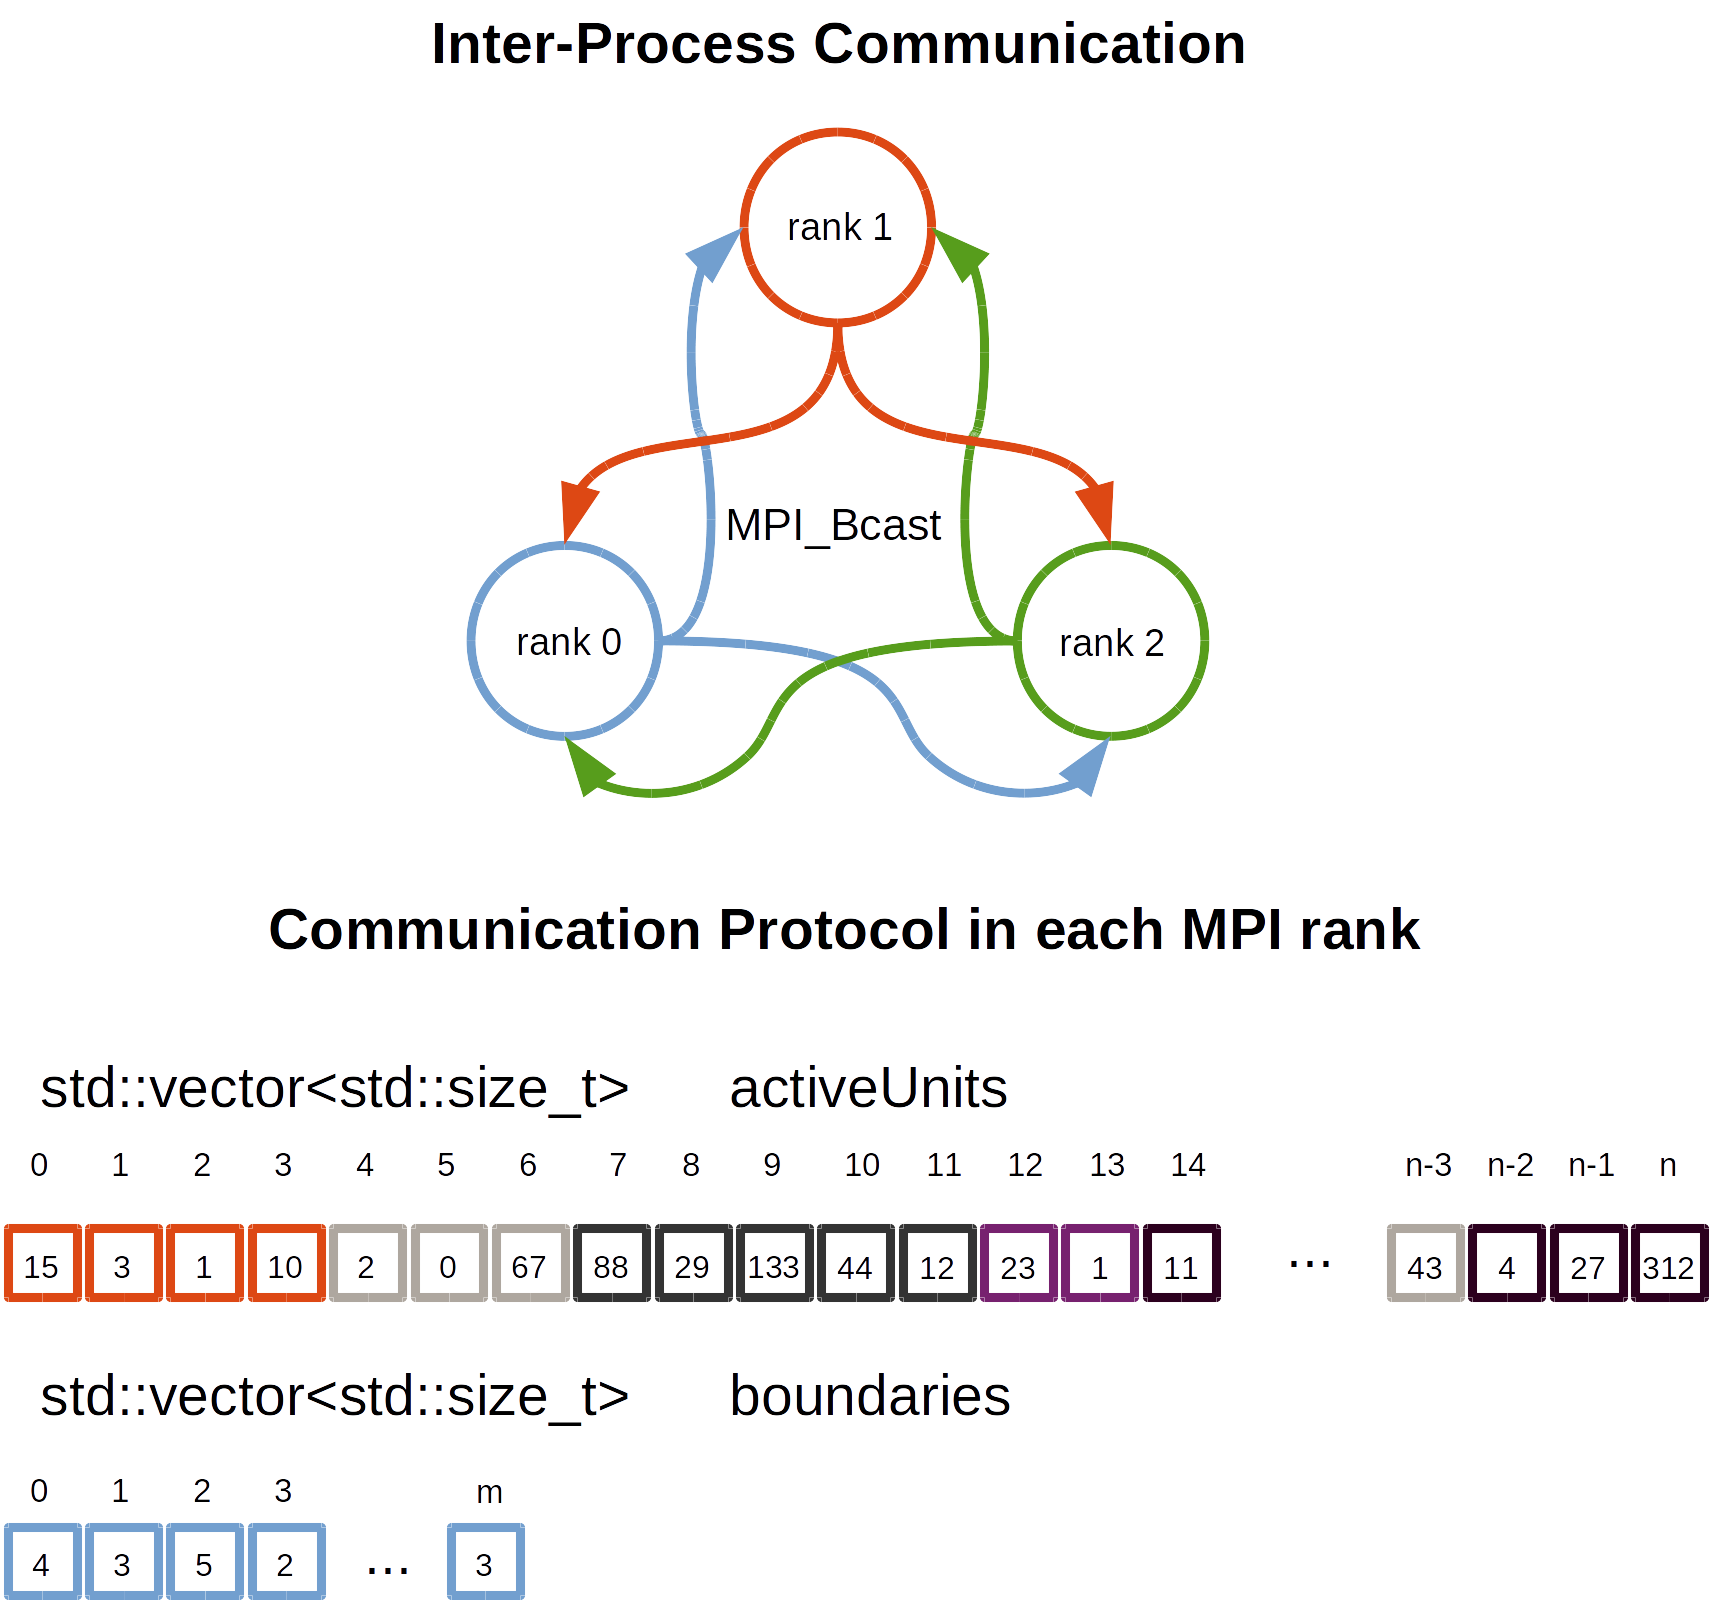
\includegraphics[width=0.6\textwidth]{BCast.png}
    \caption{Communication protocol to transmit information among \gls{mpi} ranks in the \gls{el}. All information is transmitted in two \gls{stl} vectors--\texttt{activeUnits} and \texttt{boundaries}. The vector \texttt{activeUnits} identifies the active neural units in the \glspl{cc} inside a \gls{mpi} rank and \texttt{boundaries} identifies the boundaries among active units that belong to different \glspl{cc}. There are $n+1$ active units in the \glspl{cc} managed by certain \gls{mpi} rank and there are $m+1$ \glspl{cc} managed by such \gls{mpi} rank.}
    \label{fig:BCast}
\end{figure}

The \gls{el} uses \gls{mpi} I/O parallel file system to save its status in Matlab/Octave format (Fig. \ref{fig:EncoderParallelization} D). Each \gls{mpi} rank gathers all the data corresponding to its \glspl{csom} in the \gls{el} and puts such data--formated in Matlab/Octave--in a \texttt{std::stringstream} class. Then such \gls{mpi} rank communicates the part of the file it will use to the other \gls{mpi} ranks in order to store the data without interfering with the other ranks in the \gls{mpi} environment. Finally, each \gls{mpi} rank saves all its data with a unique call to \gls{mpi} Write using the complete \texttt{std::stringstream}.

In response to biological plausibility demands for future simulations of this model, our computational approach is intended to be applied in leadership supercomputers. In this work an essential step is to test our code in order to see how it uses the resources provided by Cooley Nodes.

Parallel scalability is a measurement that indicates how efficient is our code when using increasing numbers of parallel processing elements--Nodes or Processes and \glspl{cpu} or Threads on Cooley. Fig. \ref{fig:Strong_Weak} shows the scaling capacity of our code in terms of run time vs. number of processing elements used for the task. In these tests we constrained the code to run one \gls{mpi} rank per Cooley node. Each \gls{mpi} rank spreads an specific number of threads through the different \glspl{cpu} in its corresponding node (Fig. \ref{fig:EncoderParallelization} A and B).

\begin{figure}[h!]
    \centering
    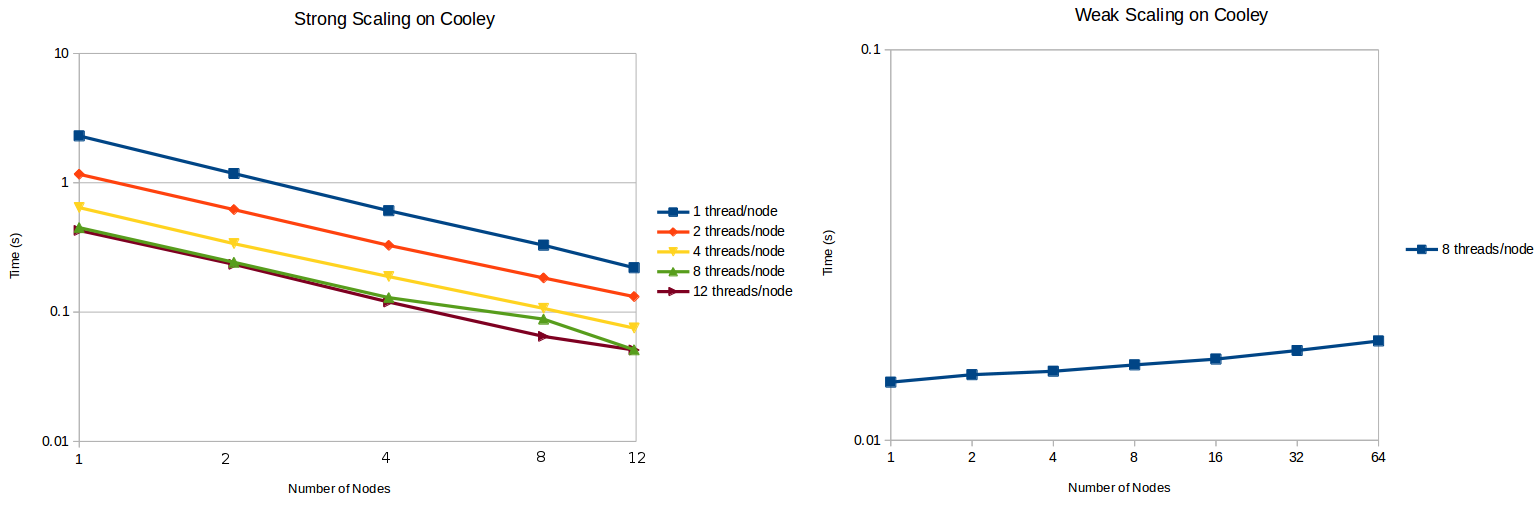
\includegraphics[width=1.0\textwidth]{Strong_Weak.png}
    \caption{Strong and Weak scaling tests on Cooley nodes. Left: Strong scaling. Run time vs. the number of nodes for different number of threads per node. The problem size stays fixed but the number of processing elements are increased. Right: Weak scaling. Run time vs. the number of nodes for 8 threads per node. In this case the problem workload assigned to each processing element stays constant and additional elements are used to solve a larger total problem (i.e. a problem that would not fit in the available RAM on a single node).}
    \label{fig:Strong_Weak}
\end{figure}

There are two ways to measure the parallel performance of a given application. The measure to be applied will depend on whether the application is \gls{cpu}-bound or memory-bound. Such measurements are referred to as \emph{strong} and \emph{weak} scaling, respectively.

Straight lines in Fig. \ref{fig:Strong_Weak} (left) show an initially good strong scalability of our code while the small slope exhibited by Fig. \ref{fig:Strong_Weak} (right) allows us to foresee a good weak scaling performance of our code in high end leadership supercomputers.

























\subsection{Corpora Generation Implementation}
\label{CorpGenImp}

%We generate a corpora of 500 words with mono, di and trisyllabic randomly chosen English words with vocabularies of five words using \gls{festival} Synthesis \cite{festival2014}.

%\begin{itemize}
	%\item Monosyllabic vocabulary: \textit{map, dog, mouse, with, truck.} % and \textit{truck}.
	%\item Disyllabic vocabulary: \textit{answer, doctor, teacher, summer, tennis.}  %and \textit{tennis}.
	%\item Trisyllabic vocabulary: \textit{computer, telephone, rectangle, tomato, magazine.} % and \textit{magazine}.
%\end{itemize}

%We generate a cross synthesizer standard mark up language file with SABLE \cite{sable}. In this file, we instruct \gls{festival} to generate a corpus with 500 words from a vocabulary of 5 words uttered by 10 different voices (8 males and 2 females) available from the synthesizer. The organization of the corpus has certain rules and restrictions in order to avoid biases in the training processes. The voices are sequentially chosen (pseudo-randomly) with the restriction that no voice could utter a second time until all the voices had uttered in their turns. Every voice utters two words per turn--in pseudo-random order--and no word is not be repeated until all the words are used by such voice. We use the following English speaking voices provided by Festival: \texttt{cmu\_us\_fem\_cg, cmu\_us\_gka\_cg, cmu\_us\_ksp\_cg, cmu\_us\_rxr\_cg, cmu\_us\_jmk\_cg, cmu\_us\_rms\_cg, cmu\_us\_slt\_cg, cmu\_us\_jmk\_arctic\_clunits, cmu\_us\_rms\_arctic\_clunits, cmu\_us\_slt\_arctic\_clunits}.

%Every word in the audio file is followed by a silence gap whose time is equivalent to the uttering time of the monosyllabic word \textit{cat}, uttered by the same voice used for the last word. We use the \texttt{text2wave} program provided by Festival in order to generate a \texttt{wav} file from the SABLE file.

We generate corpora with randomly chosen English mono and multisyllabic words using \gls{festival} Synthesis \cite{festival2014}. To that end, we generate cross synthesizer standard mark up language SABLE \cite{sable} files. In those files, we instruct \gls{festival} to generate audio \texttt{wav} files with the corpora uttered by different voices available from the synthesizer.

All the code that generates the corpora is implemented in Python and parallelized by means of a \gls{mpi} for Python package called \texttt{mpi4py}. The algorithmic implementation of this parallelization is shown in Alg.~\ref{corpora_generation_parallelization} and Fig.~\ref{fig:CorporaGenerationParallelization}.

\begin{algorithm}
	\caption{This algorithm distributes vocabularies among \gls{mpi} processes. In this algorithm we run one \gls{mpi} process per \gls{cpu} on Cooley.}
\label{corpora_generation_parallelization}
\begin{algorithmic}[1]
	\STATE {\texttt{numberOfProcesses} = getNumberOfProcesses()}
	\STATE {\texttt{processNumber} = getProcessNumber()}
	\FOR{\texttt{vocabulary} = 0 \TO \texttt{vocabulary} = \texttt{numberOfVocabularies}}
		\IF{\texttt{corpus}\%\texttt{numberOfProcesses}==\texttt{processNumber}}
			\FOR{\texttt{corpus} = 0 \TO \texttt{corpus} = \texttt{numberOfCorpora}}
				\STATE {Call \gls{festival} to generate an audio file from this \texttt{corpus} from this \texttt{vocabulary}...}
			\ENDFOR
		\ENDIF
	\ENDFOR
\end{algorithmic}
\end{algorithm}

\begin{figure}[h!]
    \centering
    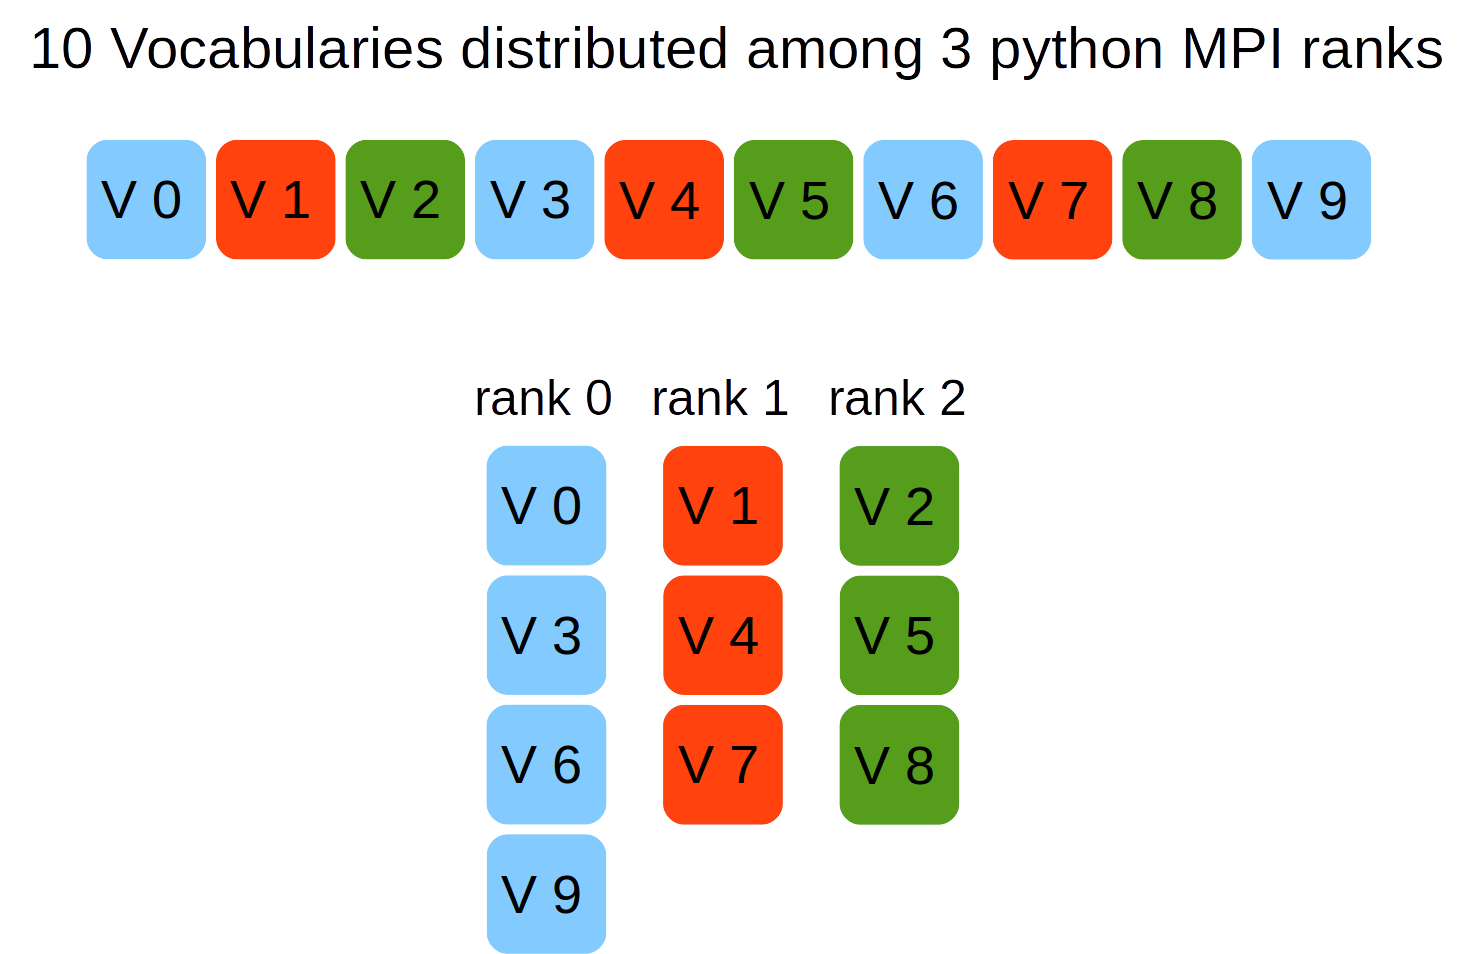
\includegraphics[width=0.4\textwidth]{CorporaGenerationParallelization.png}
    \caption{Distribution of corpora generation among Python \gls{mpi} ranks. The corpora generation tasks are distributed among Python \gls{mpi} ranks as a deck of cards is distributed among players. Each \gls{mpi} rank will end up with a set of vocabularies to generate the corpora corresponding to such vocabularies (i.e. if we have 10 corpora per vocabulary, rank 0 will end up generating 40 corpora serially while ranks 1 and 2 will generate 30 corpora each serially.}
    \label{fig:CorporaGenerationParallelization}
\end{figure}

In terms of Strong scaling (Fig.~\ref{fig:CorporaGenerationStrongScaling}), we run the algorithm in order to create 64 corpora from 64 vocabularies--one corpus per vocabulary. The code generates 64 cross synthesizer SABLE text files and then calls to Festival using \texttt{text2wav} script in order to generate the audio \texttt{wav} files which utter the text in the SABLE files.

\begin{figure}[h!]
    \centering
    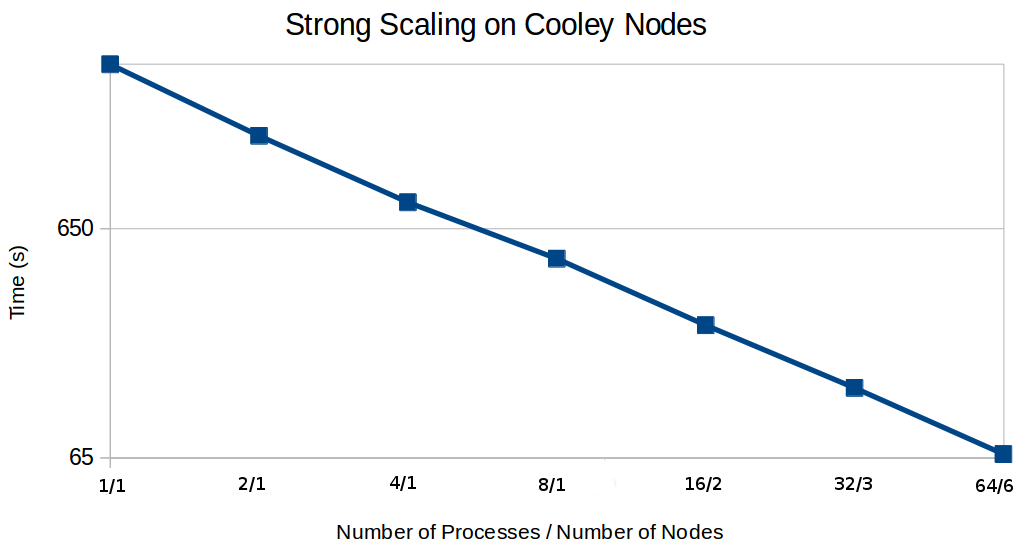
\includegraphics[width=0.5\textwidth]{CorporaGenerationStrongScaling.png}
    \caption{Strong scaling test on Cooley nodes. Run time vs. the number of \glspl{cpu}. The problem size stays fixed, that is, the run has to generate 64 corpora. On the other hand the number of processing elements is increased from 1 to 64 \glspl{cpu} in powers of two. Since Cooley nodes have 12 \glspl{cpu} we had to ask for 2 nodes in order to run on 16 \glspl{cpu}, 3 nodes in order to run on 32 \glspl{cpu} and 6 nodes in order to run on 64 \glspl{cpu}.}
    \label{fig:CorporaGenerationStrongScaling}
\end{figure}

The straight line in Fig.~\ref{fig:CorporaGenerationStrongScaling} shows a really good scaling of our code. Nevertheless, we have to take into account that each process produces an independent set of corpora and does not need to transmit any data to other processes in the \gls{mpi} session. Then, we do not have \gls{ipc} issues in this code (this is pure parallelization). Since one Cooley Node has 12 \glspl{cpu} we just needed 1 node in order to run 1, 2, 4 or 8 processes, 2 nodes (24 \glspl{cpu}) in order to run 16 processes, 3 nodes (36 \glspl{cpu}) in order to run 32 processes and finally 6 nodes (72 \glspl{cpu}) in order to run 64 processes. Another issue to take into account is that to make this code scale in the way showed by the chart, all the corpora have to have the same size, otherwise--and since the code distributes corporas on different processes in static way--some processes which take over smaller corpora would finish before other processes that take over larger corpora and would waste processing power waiting idly for other processes to finish. We have to think in a way to make the distribution of vocabularies on processes dynamic--such as \gls{omp} dynamic schedule.

In reference to Weak scaling (Fig.~\ref{fig:CorporaGenerationWeakScaling}), we generate one corpus per process, the horizontal line shows that this code scales very well  in terms of weak scaling too.

\begin{figure}[h!]
    \centering
    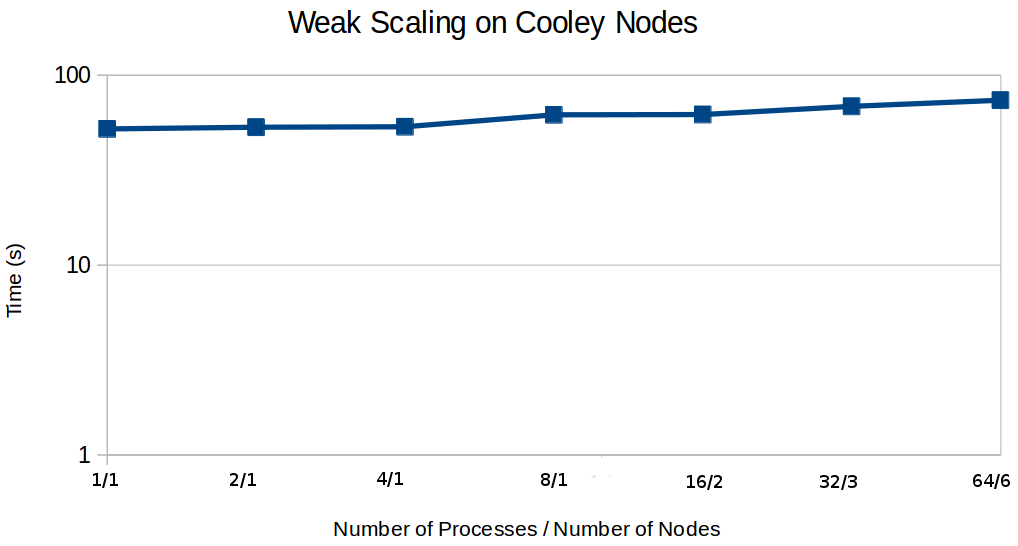
\includegraphics[width=0.5\textwidth]{CorporaGenerationWeakScaling.png}
    \caption{Weak scaling test on Cooley nodes. Run time vs. the number of \glspl{cpu}. In this case the problem workload assigned to each processing element stays constant and additional elements are used to solve a larger total problem (i.e. as we add more \glspl{cpu} we add more corpora in a way that one corpus is generated by \gls{cpu}).}
    \label{fig:CorporaGenerationWeakScaling}
\end{figure}
























\subsection{\gls{mrstsa} Implementation}

This algorithm has been implemented in C using the package called FFTW~\cite{fftw} which is an implementation of \gls{fft} available on Cooley. We used \gls{mpi}-\gls{omp} hybrid parallelization approach. We parallelized the \gls{mrstsa} algorithm developed in \cite{dematties2018} by means of \gls{omp} sections using one \gls{omp} section per spectral resolution and running until 5 \gls{omp} threads per Cooley node (Alg. ~\ref{MRSTSA_parallelization}). In terms of \gls{mpi} we processed a set of corpora per \gls{mpi} rank. The algorithm generates certain number of corpora per vocabulary. Supposing that we have $n$ vocabularies and $m$ corpora per vocabulary, we end up with $n m$ corpora. Unlike the corpora generation parallelization algorithm exposed in Alg.~\ref{fig:CorporaGenerationParallelization} and explained in section~\ref{CorpGenImp} in this case we unroll the nested loop that iterates through corpora and vocabularies. The \gls{mpi} parallelization is exposed in Alg~\ref{input_generation_parallelization}

%This algorithm has been implemented in C using the package called FFTW~\cite{fftw} which is an implementation of \gls{fft} available on Cooley. We used \gls{mpi}-\gls{omp} hybrid parallelization approach. We parallelized the algorithm explained in section \ref{mrstsa} by means of \gls{omp} sections using one \gls{omp} section per spectral resolution and running until 5 \gls{omp} threads per Cooley node (Alg. ~\ref{MRSTSA_parallelization}). In terms of \gls{mpi} we processed a set of corpora per \gls{mpi} rank. The algorithm generates certain number of corpora per vocabulary. Supposing that we have $n$ vocabularies and $m$ corpora per vocabulary, we end up with $n m$ corpora. Unlike the corpora generation parallelization algorithm exposed in Alg.~\ref{fig:CorporaGenerationParallelization} and explained in section~\ref{CorpGenImp} in this case we unroll the nested loop that iterates through corpora and vocabularies. The \gls{mpi} parallelization is exposed in Alg~\ref{input_generation_parallelization}

\begin{algorithm}
	\caption{This algorithm is called \gls{mrstsa} and distributes the different spectral resolutions--processing a corpus--among \gls{omp} threads running until 5 \gls{omp} threads concurrently in order to generate such corpus processing.}
\label{MRSTSA_parallelization}
\begin{algorithmic}[1]
	\STATE {\#\bf{pragma omp parallel sections}}
	\STATE {~~\#\bf{pragma omp section}}
	\STATE {~~~~Do stuff...}
	\STATE {~~\#\bf{pragma omp section}}
	\STATE {~~~~Do stuff...}
	\STATE {~~\#\bf{pragma omp section}}
	\STATE {~~~~Do stuff...}
	\STATE {~~\#\bf{pragma omp section}}
	\STATE {~~~~Do stuff...}
	\STATE {~~\#\bf{pragma omp section}}
	\STATE {~~~~Do stuff...}
\end{algorithmic}
\end{algorithm}

\begin{algorithm}
	\caption{This algorithm distributes corpora among \gls{mpi} processes and each \gls{mpi} process run until 5 \gls{omp} threads concurrently in order to generate each corpus. In this algorithm we run one \gls{mpi} process per Cooley node.}
\label{input_generation_parallelization}
\begin{algorithmic}[1]
	\STATE {\texttt{numberOfProcesses} = getNumberOfProcesses()}
	\STATE {\texttt{processNumber} = getProcessNumber()}
	\FOR{\texttt{task} = 0 \TO \texttt{task} = \texttt{numberOfVocabularies} * \texttt{numberOfCorpora}}
		\STATE {\texttt{corpus} = (\texttt{int})\texttt{task}/\texttt{numberOfVocabularies}}
		\STATE {\texttt{vocabulary} = \texttt{task}\%\texttt{numberOfVocabularies}}
		\STATE {MRSTSA(\texttt{corpus}, \texttt{vocabulary})}
	\ENDFOR
\end{algorithmic}
\end{algorithm}

The complete parallelization scheme is depicted in Fig.~\ref{fig:MRSTSA_Parallelization}. Corpora are distributed among \gls{mpi} ranks as a deck of cards is distributed among players. Each \gls{mpi} rank ends up with a set of corpora which it processes one at a time--sequentially. Each corpus processing runs 5 \gls{omp} threads concurrently in order to process the spectral resolutions of the corpus. 

\begin{figure}[h!]
    \centering
    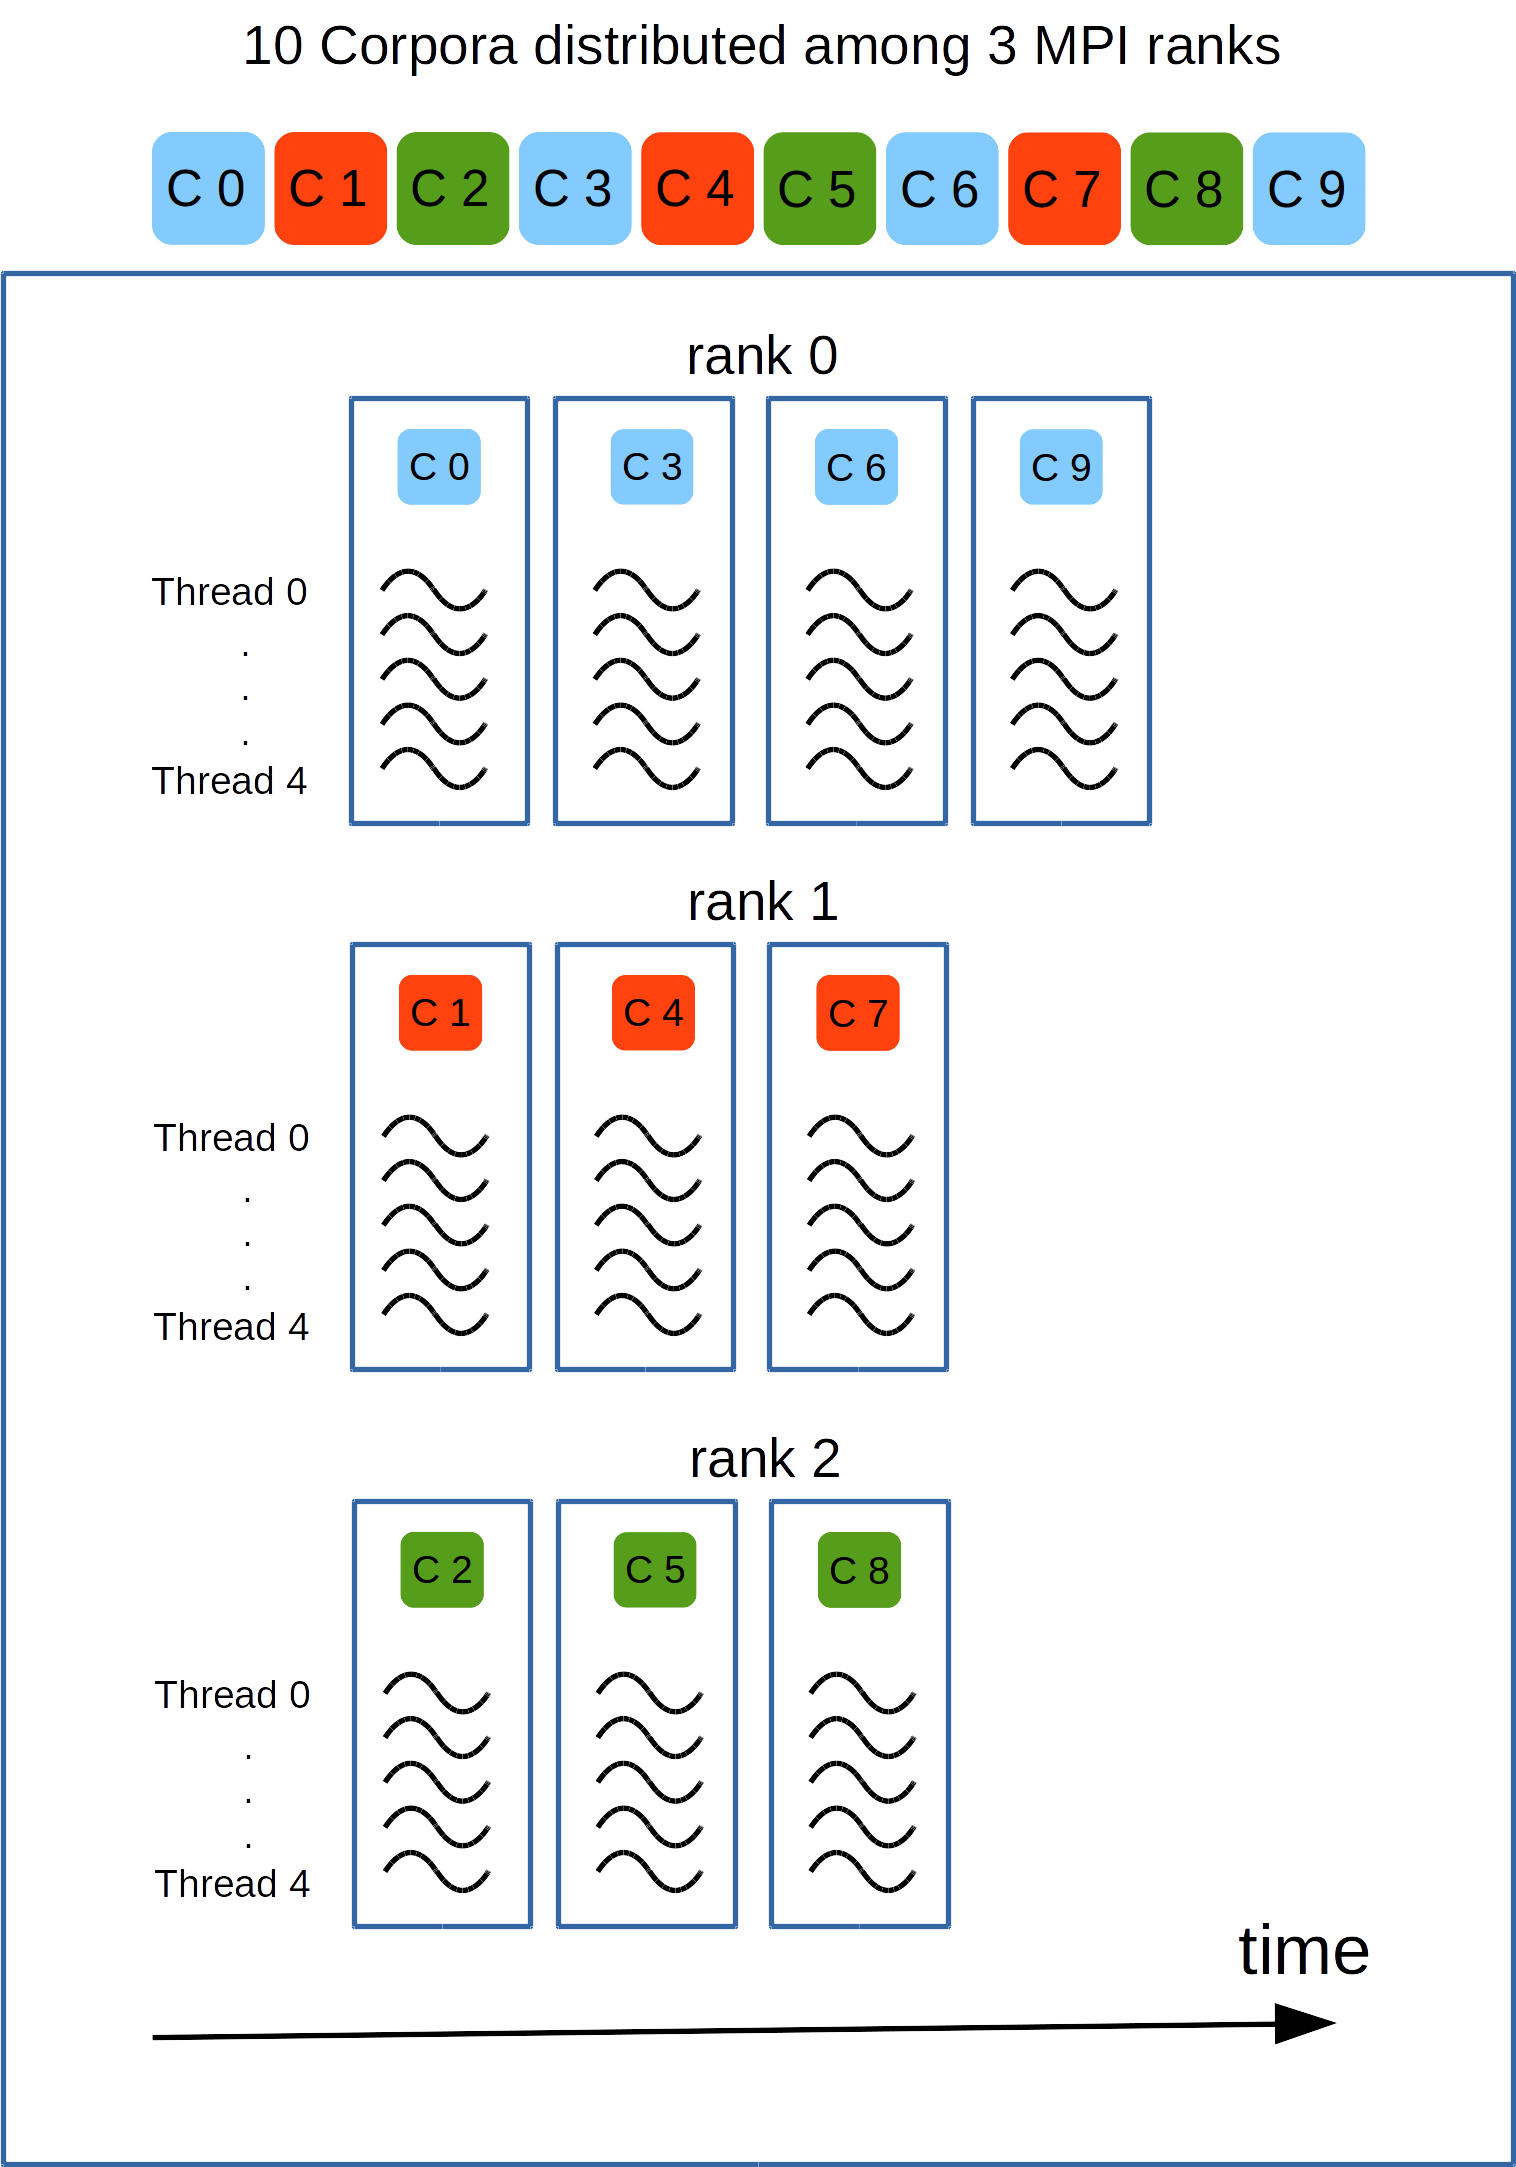
\includegraphics[width=0.4\textwidth]{MRSTSA_Parallelization.png}
    \caption{Parallelization scheme for the \gls{mrstsa}. Ten corpora processing are distributed among \gls{mpi} ranks. Each rank processes one corpus at a time sequentially but each corpus spectral resolution is processed concurrently by means of \gls{omp} threads.}
    \label{fig:MRSTSA_Parallelization}
\end{figure}

We tested the scaling capacity of this code on Cooley nodes. In terms of Strong scaling, we run the algorithm in order to process 64 corpora--one corpus per vocabulary. The straight lines in Fig.~\ref{fig:MRSTSA_Scaling}--on the left--show a really good scaling of this code. Even though, we have to take into account that each process/node computes an independent set of corpora and do not need to transmit the data to other processes/nodes in the \gls{mpi} session, we do not have \gls{ipc} issues in this code. 

\begin{figure}[h!]
    \centering
    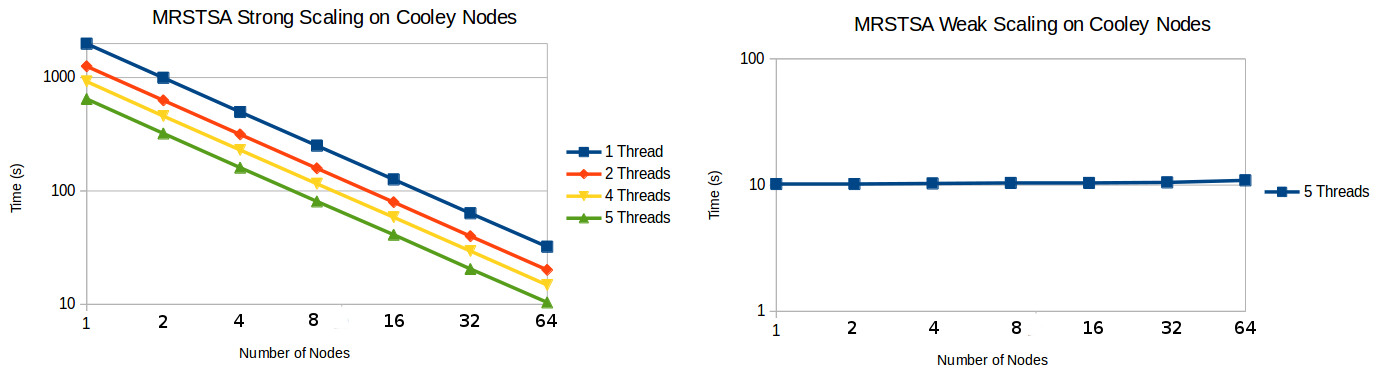
\includegraphics[width=1.0\textwidth]{MRSTSA_Scaling.png}
    \caption{Strong and Weak scaling tests on Cooley nodes. Left: Strong scaling. Run time vs. the number of nodes for different number of threads per node. The problem size stays fixed--64 corpora processing by means of \gls{mrstsa} algorithm--but the number of processing elements are increased. Right: Weak scaling. Run time vs. the number of nodes for 5 threads per node. In this case the problem workload assigned to each processing element stays constant and additional elements are used to solve a larger total problem (i.e. we add more corpora for process as the number of nodes increases in such a way that each node has to process only one corpora).}
    \label{fig:MRSTSA_Scaling}
\end{figure}

Each process run in a different node. We use an amount of \gls{omp} threads which ranges from 1 to 5. Five is the number of spectral components in the \gls{mrstsa} algorithm. Another issue to take into account is that in order to make this code scale in the way showed by the chart, all the corpora have to have the same size, otherwise--and since the code distributes corporas on different processes in static way--some processes which take over smaller corpora would finish before other processes that take over larger corpora. We have to think in a way to make the distribution of corpora on processes dynamic--such as \gls{omp} dynamic schedule.

In reference to Weak scaling, we generate one corpus per process, the horizontal line shows that this code scales very well  in terms of weak scaling too.



















































































%\subsubsection{Static Self Organizing Map Class}

%\begin{algorithm}
	%\caption{\texttt{getResponse} method. This method returns the euclidean distances between the \texttt{input} vector and
	%each unit \texttt{weights} vector as well as a vector with the \texttt{ranking} of units proximity to the input vector.}
%\label{ssom_getResponse}
%\begin{algorithmic}[1]
	%\FOR{\texttt{unit} = 0 \TO \texttt{unit} = number of units }
	%\STATE {\texttt{distances[unit]} = distance between \texttt{weights[unit]} and \texttt{input}}
	%\ENDFOR
	%\STATE {\texttt{ranking} = sort indexes from the smallest to the largest \texttt{distances}}
	%\RETURN \texttt{distances}, \texttt{ranking}
%\end{algorithmic}
%\end{algorithm}

%\begin{algorithm}
	%\caption{\texttt{learningRule} method. This method updates the \texttt{weights} in the Static Self Organizing Map in the presence of a new \texttt{input} vector.}
%\label{ssom_learningRule}
%\begin{algorithmic}[1]
	%\FOR{\texttt{unit} = 0 \TO \texttt{unit} = number of units }
		%\STATE {\texttt{neighborhood} value = neighborhood measure between unit \texttt{winner} position and \texttt{unit} position (\texttt{learningNeighborhood} method)}
		%\STATE {\texttt{weights[unit]} = \texttt{weights[unit]} + learning rate*\texttt{neighborhood} value*(\texttt{input} - \texttt{weights[unit]})}
	%\ENDFOR
%\end{algorithmic}
%\end{algorithm}

%\begin{algorithm}
	%\caption{\texttt{learningNeighborhood} method. This method computes a measure of the neighborhood between two units.}
%\label{ssom_learningNeighborhood}
%\begin{algorithmic}[1]
	%\STATE {\texttt{winner} position on array = return position of \texttt{winner unit} on the \emph{unit array dimensionality}}
	%\STATE {\texttt{other position} on array = return position of \texttt{other unit} on the \emph{unit array dimensionality}}
	%\FOR{\texttt{index} = 0 \TO \texttt{index} = number of array dimensions }
		%\STATE {\texttt{auxiliary[index]} = |\texttt{winner position[index]}-\texttt{other position[index]}|}
	%\ENDFOR
	%\STATE {\texttt{distance} = accumulate \texttt{auxiliary} components}
	%\RETURN {exp(-(pow(\texttt{distance}, 2)) / (2*width parameter))}
%\end{algorithmic}
%\end{algorithm}








%\subsubsection{Static Processor Class}

%\begin{algorithm}
	%\caption{\texttt{getResponse} method. This method returns the units \texttt{excitation} vector
	%as well as a vector with the \texttt{ranking} of units \texttt{excitation}.}
%\label{sproc_getResponse}
%\begin{algorithmic}[1]
	%\FOR{\texttt{unit} = 0 \TO \texttt{unit} = number of units }
		%\STATE{\texttt{inner} product = 0}
		%\FOR{\texttt{input} index in \texttt{input} indexes}
			%\STATE{\texttt{potential} index = find the first coincident index in \texttt{potential[unit]} connections with \texttt{input} index}
			%\IF{ there is coincidence }
				%\STATE {\texttt{inner} product = \texttt{inner} product + \texttt{weights[unit][potential \textnormal{index}]}}
			%\ENDIF
		%\ENDFOR
		%\STATE{\texttt{excitation[unit]} = \texttt{inner} product}
	%\ENDFOR
	%\STATE{\texttt{ranking} = sort indexes by the level of \texttt{excitation} (from the smallest to the largest)}
	%\RETURN \texttt{excitation}, \texttt{ranking}
%\end{algorithmic}
%\end{algorithm}




%\begin{algorithm}
	%\caption{\texttt{learningRule} method. This method updates the weights in the Static Processor in the presence of a new \texttt{input}.}
%\label{sproc_learningRule}
%\begin{algorithmic}[1]
	%\STATE{\texttt{excitation}, \texttt{ranking} = gets the units \texttt{excitation} as well as the \texttt{ranking} in its excitation in response to the \texttt{input} vector (\texttt{getResponse} method)}
	%\STATE{number of affected units = plasticity*number of units}
	%\IF{activation homeostasis is enabled}
		%\STATE{modulated \texttt{excitation} = element wise multiplication between \texttt{excitation} vector and activation \texttt{busting}}
		%\IF{randomness is disabled}
			%\STATE {modulated \texttt{ranking} = sort indexes by the level of modulated \texttt{excitation} (from the smallest to the largest)}
			%\STATE {unit winner \texttt{positions} = the last \emph{number of affected units} elements in modulated \texttt{ranking}}
		%\ELSE
			%\STATE {unit winner \texttt{positions} = gets \emph{number of affected units} random indexes from modulated \texttt{excitation} with probabilities determined by the relative \texttt{excitation} element values}
		%\ENDIF
	%\ELSE
		%\IF{randomness is disabled}
			%\STATE {unit winner \texttt{positions} = the last \emph{number of affected units} elements in \texttt{ranking}}
		%\ELSE
			%\STATE {unit winner \texttt{positions} = gets \emph{number of affected units} random indexes from \texttt{excitation} with probabilities determined by the relative \texttt{excitation} element values}
		%\ENDIF
	%\ENDIF

%%\algstore{part1}
%\end{algorithmic}
%\end{algorithm}


%\begin{algorithm}
%\ContinuedFloat
	%\caption{\texttt{learningRule} method. This method updates the weights in the Static Processor in the presence of a new \texttt{input}.}
%\label{sproc_learningRule}
%\begin{algorithmic}[1]
%%\algrestore{part1}
	%\FOR{unit winner \texttt{position} in unit winner \texttt{positions}}
		%\FOR{\texttt{unit} = 0 \TO \texttt{unit} = number of units }
			%\STATE {\texttt{neighborhood} value = neighborhood measure between unit winner \texttt{position} and \texttt{unit} position (\texttt{learningNeighborhood} method)}
			%\STATE{~~}
			%\IF{\texttt{neighborhood} value > PROXIMAL\_SYNAPTIC\_THRESHOLD}
				%\STATE{\texttt{increment} = learning rate*\texttt{neighborhood} value*SYNAPTIC\_INCREMENT}
				%\STATE{\texttt{decrement} = learning rate*\texttt{neighborhood} value*SYNAPTIC\_DECREMENT}
				%\STATE{~~}
				%\FOR{\texttt{input} index in \texttt{input} indexes}
					%\STATE{\texttt{potential} index = find the first coincident index in \texttt{potential[unit]} connections with \texttt{input} index}
					%\IF{ there is coincidence }
						%\STATE {\texttt{weights[unit][potential \textnormal{index}]} += \texttt{increment}}
						%\STATE {incorporates \texttt{potential} index to the list of \texttt{potential} indexes}
					%\ENDIF
				%\ENDFOR
				%\STATE{~~}
				%\IF{ENABLE\_RANDOM\_BEHAVIOUR is true and \texttt{weights[unit]} sparsity is false}
					%\STATE{number of affected synapses = MASSIVE\_PLASTICITY*number of potential connections}
					%\FOR{random \texttt{choice} = 0 \TO random \texttt{choice} = number of affected synapses }
						%\STATE{\texttt{choice} = random integer between 0 and number of potential connections - 1}
						%\STATE{security scape = 0}
						%\WHILE{\texttt{choice} is in the list of \texttt{potential} indexes or \texttt{choice} is in the list of \texttt{inactive} indexes}

							%\STATE{\texttt{choice} = random integer between 0 and number of potential connections - 1}
							%\IF{security scape > 10\% of the number of components in the \texttt{input} vector}
								%\STATE {break the while loop}
							%\ENDIF
							%\STATE{security scape++}
						%\ENDWHILE
						%\STATE{incorporates \texttt{choice} to the list of \texttt{inactive} indexes}
						%\IF{\texttt{weights[unit][choise]} > 0}
							%\STATE{\texttt{weights[unit][choise]} -= \texttt{decrement}}
							%\IF{\texttt{weights[unit][choise]} < 0}
								%\STATE {\texttt{weights[unit][choise]} < 0}
							%\ENDIF
						%\ENDIF
					%\ENDFOR
				%\ENDIF
				%\STATE{~~}
			%\ENDIF
			%\STATE{~~}
		%\ENDFOR
	%\ENDFOR
%%\algstore{part2}
%\end{algorithmic}
%\end{algorithm}


%\begin{algorithm}
%\ContinuedFloat
	%\caption{\texttt{learningRule} method. This method updates the weights in the Static Processor in the presence of a new \texttt{input}.}
%\label{sproc_learningRule}
%\begin{algorithmic}[1]
%%\algrestore{part2}
	%\FOR{units winner \texttt{position} in units winner \texttt{positions}}
	%\STATE {units \texttt{activity[\textnormal{units winner} position]++}}
	%\ENDFOR
%\end{algorithmic}
%\end{algorithm}


%\begin{algorithm}
	%\caption{\texttt{activationHomeostasis} method. This method computes activation homeostasis over the units.}
%\label{sproc_activationHomeostasis}
%\begin{algorithmic}[1]
	%\STATE{average \texttt{activity} = gets average of units \texttt{activity}}
	%\FOR{\texttt{unit} = 0 \TO \texttt{unit} = number of units }
		%\IF{updated \texttt{step} > 0}
			%\STATE {activation \texttt{boosting[unit]} = exp(-boosting factor*(units \texttt{activity[unit]}-average \texttt{activity})/updated \texttt{step})}
		%\ELSE
			%\STATE {activation \texttt{boosting[unit]} = exp(-boosting factor*(units \texttt{activity[unit]}-average \texttt{activity}))}
		%\ENDIF
	%\ENDFOR
%\end{algorithmic}
%\end{algorithm}


%\begin{algorithm}
	%\caption{\texttt{synapticGrowthLimitation} method. This method computes synaptic growth limitation over the weights.}
%\label{sproc_synapticGrowthLimitation}
%\begin{algorithmic}[1]
	%\FOR{\texttt{unit} = 0 \TO \texttt{unit} = number of units }
		%\STATE{\texttt{sum} = sum all elements in \texttt{weights[unit]}}
		%\IF{\texttt{sum} > 1}
			%\STATE {\texttt{weights[unit]/sum}}
		%\ENDIF
		%\STATE{sets all the elements in \texttt{weights[unit]} whose value is below the synaptic \texttt{threshold} to 0}
	%\ENDFOR
%\end{algorithmic}
%\end{algorithm}


%\begin{algorithm}
	%\caption{\texttt{synapticHomeostasis} method. This method computes synaptic homeostasis over the weights.}
%\label{sproc_synapticHomeostasis}
%\begin{algorithmic}[1]
	%\STATE{average \texttt{activity} = gets average of units \texttt{activity}}
	%\STATE{apply synaptic growth limitation with certain synaptic \texttt{threshold} (\texttt{synapticGrowthLimitation} method)}
	%\STATE{~~}
	%\FOR{\texttt{unit} = 0 \TO \texttt{unit} = number of units }
		%\IF{units \texttt{activity[unit]} is below the 10 \% of the average \texttt{activity}}
			%\STATE{neighbor \texttt{units} = gets all unit indexes whose hamming distance to \texttt{unit} is 1 in the units array dimensionality}
			%\STATE{~~}
			%\FOR{neighbor \texttt{unit} in neighbor \texttt{units}}
				%\STATE {\texttt{weights[unit]} += \texttt{weights[\textnormal{neighbor} unit]}}
			%\ENDFOR
			%\STATE{~~}
			%\IF{ENABLE\_RANDOM\_BEHAVIOUR is true}
				%\STATE{number of \texttt{choises} = MASSIVE\_PLASTICITY*number of potential connections}
				%\FOR{random \texttt{choice} \TO random \texttt{choice} = number of \texttt{choises} }
					%\STATE{\texttt{choice} = random integer between 0 and number of potential connections - 1}
					%\STATE{security scape = 0}
					%\WHILE{\texttt{choice} is in the list of random \texttt{choices}}
						%\STATE{\texttt{choice} = random integer between 0 and number of potential connections - 1}
						%\IF{security scape > 10\% of the number of components in the \texttt{input} vector}
							%\STATE {break the while loop}
						%\ENDIF
						%\STATE{security scape++}
					%\ENDWHILE
					%\STATE{incorporates \texttt{choice} to the list of random \texttt{choices}}
					%\STATE{\texttt{weights[unit][choise]} += get random real number between SYNAPTIC\_DECREMENT and SYNAPTIC\_INCREMENT}
				%\ENDFOR
			%\ENDIF
			%\STATE{~~}
		%\ENDIF
	%\ENDFOR
%\end{algorithmic}
%\end{algorithm}


%\begin{algorithm}
	%\caption{\texttt{homeostasis} method. This method applies homeostasis to the object.}
%\label{sproc_homeostasis}
%\begin{algorithmic}[1]
%\IF{activation homeostasis is enabled and updated \texttt{step} module 5 is 0}
	%\STATE {applies activation homeostasis with a boosting factor of 10*BOOSTING (\texttt{activationHomeostasis} method)}
%\ENDIF
%\STATE{~~}
%\IF{updated \texttt{step} > UPDATE\_PERIOD}
	%\IF{learning is enabled}
		%\IF{synaptic homeostasis is enabled}
			%\STATE {applies synaptic homeostasis with synaptic \texttt{threshold} (\texttt{synapticHomeostasis} method)}
		%\ELSE
			%\STATE {applies synaptic grow limitation  with synaptic \texttt{threshold} (\texttt{synapticGrowthLimitation} method)}
		%\ENDIF
	%\ENDIF
	%\STATE{minimum \texttt{activity} = gets the minimum activity from units \texttt{activity}}
	%\STATE{units \texttt{activity} -= minimum \texttt{activity}}
	%\FOR{\texttt{unit} = 0 \TO \texttt{unit} = number of units }
		%\STATE {\texttt{weights[unit]} sparsity = (sparsity in \texttt{weights[unit]} > SPARSITY\_THRESHOLD)}
	%\ENDFOR
	%\STATE{updated \texttt{step} = 0}
%\ENDIF
%\STATE{updated \texttt{step}++}
%\end{algorithmic}
%\end{algorithm}

%\subsubsection{Dynamic Self Organizing Map Class}

%\begin{algorithm}
	%\caption{\texttt{getDynamicResponse} method. This method modifies response using the dynamic \texttt{synapses}.}
%\label{dsom_getDynamicResponse}
%\begin{algorithmic}[1]
	%\FOR{\texttt{unit} = 0 \TO \texttt{unit} = number of units }
		%\STATE{auxiliary = 0}
		%\FOR{\texttt{dendrite} = 0 \TO \texttt{dendrite} = number of dendrites }
			%\STATE{\texttt{dendrite} accumulator = 0}
			%\FOR{\texttt{synapse} = 0 \TO \texttt{synapse} = number of synapses }
				%\STATE{potential \texttt{index} = find the first coincident index in potential \texttt{connections[dendrite][unit]} with linking \texttt{units[dendrite][connection]}}
				%\IF{there exist coincidence}
					%\STATE {\texttt{dendrite} accumulator += dynamic \texttt{synapses[dendrite][unit][\textnormal{potential} index]}}
				%\ENDIF
			%\ENDFOR
			%\IF{\texttt{dendrite} accumulator > 100*DISTAL\_SYNAPTIC\_THRESHOLD}
				%\STATE {auxiliary++}
			%\ENDIF
		%\ENDFOR
		%\STATE{total \texttt{responses[unit]} += auxiliary}
	%\ENDFOR
	%\STATE{\texttt{distances} = \texttt{distances}/total \texttt{responses[unit]}}
	%\STATE {\texttt{ranking} = sort indexes from the smallest to the largest \texttt{distances}}
	%\RETURN \texttt{distances}, \texttt{ranking}
%\end{algorithmic}
%\end{algorithm}


%\begin{algorithm}
	%\caption{\texttt{Update} method. This method updates a group of dynamic \texttt{synapses} depending on a set of unit indexes. Every link -from which information is coming- is a vector, hence it could contain a set of linking units as well as a unique linking unit.}
%\label{dsom_Update}
%\begin{algorithmic}[1]
%\IF{increment is true}
	%\FOR{index in indexes}
		%\FOR{dendrite = 0 \TO dendrite = number of dendrites }
			%\FOR{connection = 0 \TO connection = number of connections in linking \texttt{units[dendrite]}}
				%\STATE{potential \texttt{index} = find the first coincident index in potential \texttt{connections[dendrite][index]} with linking \texttt{units[dendrite][connection]}}
				%\IF{there exist coincidence}
					%\STATE {dynamic \texttt{synapses[dendrite][index][\textnormal{potential} index]} += learning rate*SYNAPTIC\_INCREMENT}
				%\ENDIF
			%\ENDFOR
		%\ENDFOR
	%\ENDFOR
%\ELSE
	%\FOR{index in indexes}
		%\FOR{dendrite = 0 \TO dendrite = number of dendrites }
			%\FOR{connection = 0 \TO connection = number of connections in linking \texttt{units[dendrite]}}
				%\STATE{potential \texttt{index} = find the first coincident index in potential \texttt{connections[dendrite][index]} with linking \texttt{units[dendrite][connection]}}
				%\IF{there exist coincidence}
					%\STATE {dynamic \texttt{synapses[dendrite][index][\textnormal{potential} index]} -= learning rate*SYNAPTIC\_DECREMENT}
					%\IF{dynamic \texttt{synapses[dendrite][index][\textnormal{potential} index]} < 0}
						%\STATE {dynamic \texttt{synapses[dendrite][index][\textnormal{potential} index]} = 0}
					%\ENDIF
				%\ENDIF
			%\ENDFOR
		%\ENDFOR
	%\ENDFOR
%\ENDIF
%\IF{updated step > UPDATE\_PERIOD}
	%\FOR{dendrite = 0 \TO dendrite = number of dendrites }
		%\FOR{\texttt{unit} = 0 \TO \texttt{unit} = number of units }
			%\STATE{\texttt{sum} = sum all elements in dynamic \texttt{synapses[dendrite][unit]}}
			%\IF{\texttt{sum} > 1}
				%\STATE{dynamic \texttt{synapses[dendrite][unit]} =/\texttt{sum}}
			%\ENDIF
			%\STATE{sets all the elements in dynamic \texttt{synapses[dendrite][unit]} whose value is below the threshold to 0}
		%\ENDFOR
	%\ENDFOR
	%\STATE{updated \texttt{step} = 0}
%\ENDIF
%\STATE{updated \texttt{step}++} 
%\end{algorithmic}
%\end{algorithm}





%\subsubsection{Dynamic Processor Class}

%\todo{This method with dendrites as independent processing elements has not yet been implemented in the repository.}
%\begin{algorithm}
	%\caption{\texttt{getDynamicResponse} method. This method modifies response using the dynamic \texttt{synapses}.}
%\label{dproc_getDynamicResponse}
%\begin{algorithmic}[1]
	%\FOR{\texttt{unit} = 0 \TO \texttt{unit} = number of units }
		%\STATE{auxiliary = 0}
		%\FOR{\texttt{dendrite} = 0 \TO \texttt{dendrite} = number of dendrites }
			%\STATE{\texttt{dendrite} accumulator = 0}
			%\FOR{\texttt{synapse} = 0 \TO \texttt{synapse} = number of synapses }
				%\STATE{potential \texttt{index} = find the first coincident index in potential \texttt{connections[dendrite][unit]} with linking \texttt{units[dendrite][connection]}}
				%\IF{there exist coincidence}
					%\STATE {\texttt{dendrite} accumulator += dynamic \texttt{synapses[dendrite][unit][\textnormal{potential} index]}}
				%\ENDIF
			%\ENDFOR
			%\IF{\texttt{dendrite} accumulator > 100*DISTAL\_SYNAPTIC\_THRESHOLD}
				%\STATE {auxiliary++}
			%\ENDIF
		%\ENDFOR
		%\STATE{total \texttt{responses[unit]} += auxiliary}
	%\ENDFOR
	%\STATE{\texttt{excitation} = \texttt{excitation}*total \texttt{responses[unit]}}
	%\STATE {\texttt{ranking} = sort indexes from the smallest to the largest \texttt{excitation}}
	%\RETURN \texttt{excitation}, \texttt{ranking}
%\end{algorithmic}
%\end{algorithm}

%\subsubsection{Complex Self Organizing Map Class}

%\begin{algorithm}
	%\caption{\texttt{Activate} method. This method decides which units in the population to activate depending on response info.}
%\label{csom_Activate}
%\begin{algorithmic}[1]
	%\STATE{minimum number of active units = (1-sparsity)*number of units}
	%\IF{randomness is disabled}
		%\STATE {excited \texttt{units} = gets the first \emph{number of excited units} elements from \texttt{ranking}}
	%\ELSE
		%\STATE {excited \texttt{units} = gets \emph{number of excited units} random indexes from \texttt{distances} with probabilities determined by the relative reciprocal of the \texttt{distances} element values}
	%\ENDIF
	%\STATE{dynamic \texttt{distances} and dynamic \texttt{ranking} = get dynamic response from \texttt{distances} and \texttt{ranking} in correspondence with linking \texttt{units}. (\texttt{getDynamicResponse} method)}
	%\STATE{new \texttt{distances} = get the \texttt{distances} elements whose indexes are in excited \texttt{units}}
	%\STATE{new minimum \texttt{distance} = get the minimum element from new \texttt{distances}}
	%\STATE{minimum \texttt{indexes} = get indexes from dynamic \texttt{distances} vector whose values are in new minimum \texttt{distances}}
	%\STATE{apt to be \texttt{active} = get the coincident indexes between excited \texttt{units} and minimum \texttt{indexes}}
	%\STATE{erase from new \texttt{distances} vector, all the elements whose value is equal to new minimum \texttt{distance}}
	%\WHILE{number of elements in apt to be \texttt{active} vector < \emph{minimum number of active units} and new \texttt{distances} has at least one element}
		%\STATE{new minimum \texttt{distance} = get the minimum element from new \texttt{distances}}
		%\STATE{minimum \texttt{indexes} = get indexes from dynamic \texttt{distances} vector whose values are in new minimum \texttt{distances}}
		%\STATE{partial apt to be \texttt{active} = get the coincident indexes between excited \texttt{units} and minimum \texttt{indexes}}
		%\STATE{incorporate partial apt to be \texttt{active} elements into apt to be \texttt{active} vector}
		%\STATE{erase from new \texttt{distances} vector, all the elements whose value is equal to new minimum \texttt{distance}}
	%\ENDWHILE
	%\IF{ENABLE\_RANDOM\_BEHAVIOUR}
		%\STATE {shuffle apt to be \texttt{active} vector}
	%\ENDIF
	%\FOR{\texttt{number} = 0 \TO \texttt{number} = number of apt to be \texttt{active} elements }
		%\STATE {incorporate to \texttt{output} the excited \texttt{units[\textnormal{apt to be} active[number]]}}
	%\ENDFOR
	%\RETURN \texttt{output}
%\end{algorithmic}
%\end{algorithm}

%\subsubsection{Complex Processor Class}

%\begin{algorithm}
	%\caption{\texttt{Activate} method. This method decides which units in the population to activate depending on response info.}
%\label{cproc_Activate}
%\begin{algorithmic}[1]
	%\STATE{minimum number of active units = (1-sparsity)*number of units}
	%\IF{randomness is disabled}
		%\STATE {excited \texttt{units} = gets the first \emph{number of excited units} elements from \texttt{ranking}}
	%\ELSE
		%\STATE {excited \texttt{units} = gets \emph{number of excited units} random indexes from \texttt{excitations} with probabilities determined by the relative \texttt{excitations} element values}
	%\ENDIF
	%\STATE{dynamic \texttt{excitations} and dynamic \texttt{ranking} = get dynamic response from \texttt{excitations} and \texttt{ranking} in correspondence with linking \texttt{units}. (\texttt{getDynamicResponse} method)}
	%\STATE{new \texttt{excitations} = get the \texttt{excitations} elements whose indexes are in excited \texttt{units}}
	%\STATE{new maximum \texttt{excitation} = get the maximum element from new \texttt{excitations}}
	%\STATE{maximum \texttt{indexes} = get indexes from dynamic \texttt{excitations} vector whose values are in new maximum \texttt{excitations}}
	%\STATE{apt to be \texttt{active} = get the coincident indexes between excited \texttt{units} and maximum \texttt{indexes}}
	%\STATE{erase from new \texttt{excitations} vector, all the elements whose value is equal to new maximum \texttt{excitation}}
	%\WHILE{number of elements in apt to be \texttt{active} vector < \emph{minimum number of active units} and new \texttt{excitations} has at least one element}
		%\STATE{new maximum \texttt{excitation} = get the maximum element from new \texttt{excitations}}
		%\STATE{maximum \texttt{indexes} = get indexes from dynamic \texttt{excitations} vector whose values are in new maximum \texttt{excitations}}
		%\STATE{partial apt to be \texttt{active} = get the coincident indexes between excited \texttt{units} and maximum \texttt{indexes}}
		%\STATE{incorporate partial apt to be \texttt{active} elements into apt to be \texttt{active} vector}
		%\STATE{erase from new \texttt{excitations} vector, all the elements whose value is equal to new maximum \texttt{excitation}}
	%\ENDWHILE
	%\IF{ENABLE\_RANDOM\_BEHAVIOUR}
		%\STATE {shuffle apt to be \texttt{active} vector}
	%\ENDIF
	%\FOR{\texttt{number} = 0 \TO \texttt{number} = number of apt to be \texttt{active} elements }
		%\STATE {incorporate to \texttt{output} the excited \texttt{units[\textnormal{apt to be} active[number]]}}
	%\ENDFOR
	%\RETURN \texttt{output}
%\end{algorithmic}
%\end{algorithm}

%\subsubsection{Encoder Layer Class}

%\begin{algorithm}
	%\caption{\texttt{interconnectEncoderLayerColumns} method. This method interconnects the layaer's populations.}
%\label{csom_interconnectEncoderLayerColumns}
%\begin{algorithmic}[1]
	%\FOR{cortical \texttt{column} = 0 \TO cortical \texttt{column} = number of cortical columns }
		%\STATE {afferent \texttt{connections[\textnormal{cortical} column]} = gets afferent inputs for cortical \texttt{column} (\texttt{getAfferentInputs} method)}
	%\ENDFOR
	%\IF{<condition>}
		%\FOR{cortical \texttt{column} = 0 \TO cortical \texttt{column} = number of cortical columns }
			%\STATE {lateral distal \texttt{connections[\textnormal{cortical} column]} = gets lateral distal inputs for cortical \texttt{column} (\texttt{getLateralDistalInputs} method)}
		%\ENDFOR
	%\ENDIF
%\end{algorithmic}
%\end{algorithm}

%\subsubsection{Regular Layer Class}

%\subsubsection{Model Class}









~\\
~\\
~\\
~\\

~\\
~\\
~\\
~\\

~\\
~\\
~\\
~\\

~\\
~\\
~\\
~\\
















\iffalse


\section{Model}


In this research we gather potentially relevant anatomical and neurophysiological features which could be significant for phonetic invariance in the mammalian auditory cortex. We test those principles using a completely unsupervised and biologically inspired computational model which returns phonetic classification accuracy levels similar to those of state-of-the-art deep pattern classification approaches.


Cortical cells are aligned into restricted domains for common receptive field locations called \glspl{cc} \cite{mountcastle_1955, mountcastle_1957, hubel_1962, hubel_1968}. Cortical mini-columns inside \glspl{cc} are clusters of cells which respond to stimuli with similar characteristics (Fig. \ref{fig:Biological}).

According to recent findings in neuroscience,
%\emph{the brain uses \glspl{sdr} to process information}
\emph{the brain processes information by means of \glspl{sdr}}
\cite{barth_2012}.
This is true for all mammals, from mice to humans. Extended depolarization of the soma could be the result of independent dendritic \gls{nmda} branch activations produced by the excitation of certain number of distal synapses \cite{antic_2010, major_2013}. Adaptation to contextual stimuli is ubiquitous in cortical tissue and is thought to enhance efficiency in the codification of sensory information. By means of a reduction in the responses to frequent sounds, complex inhibitory networks may enhance cortical sensitivity to rare sounds that may represent unexpected events \cite{Natan2015ComplementaryCO,nachum_2003,Javitt11962}.

\subsection*{Model}
We propose a computational approach called \gls{cstm}, which simulates a patch of cortical tissue and incorporates columnar organization, spontaneous micro-columnar formation, and partial \gls{nmda} depolarization and adaptation to contextual activations. We simulate pyramidal cells with proximal connections from afferent dendritic branches and distal connections from lateral dendritic branches. Similar afferent stimuli activate clusters of neurons with proximal physical locations in a \gls{cc} in the same way that afferent information activates the mini columns found in cortical tissue.

Afferent information activates different clusters of units in a \gls{cc} establishing a first and raw approximation of the phonetic features abstracted from the input auditory stream. Our model fine-tunes such raw features by means of previous contextual activations produced in the same and/or in neighboring \glspl{cc}. Such contextual information is sent to each \gls{cc} by means of lateral distal dendritic branches which work as independent processing elements in a cell. Current activation in such dendritic elements will affect the way in which cells receives future afferent information.

Novel computational theories have posited a feasible explanation about the role of distal synapses related to \gls{nmda}
phenomenon \cite{hawkins_2016} by combining it with \glspl{sdr} \cite{ahmad_2016}. In our model, we adopt a similar approach to the one in \cite{hawkins_2016} in which current activation patterns produce partial depolarization of certain cells by means of distal dendritic branch connections. A state of partial depolarization is sustained in time in some cells within
future afferently excited clusters of neurons. Cells fire in advance with respect to other cells in the excited clusters, thereby preventing other cells from firing by means of proximal lateral GABAergic inhibition, obtaining in this way, \glspl{sdr}.

In addition, we simulate the growth of distal dendritic branch synapses by means of \gls{stdp} mechanisms together with
homeostatic regulations. In this way, distal synapses will be established only among pyramidal cells with sequential patterns
of activation. Afferently excited clusters which do not have partially depolarized cells,
will fire together producing a \gls{mfe}
(lack of inhibition) as a response to a prediction fault (unexpected sequential stimuli in the stream of data); otherwise they will respond with normal firing events (inhibition and therefore \glspl{sdr}) when the sequential stimulus is
correctly predicted.

\glspl{sdr} exhibit interesting mathematical properties which give them high noise rejection and fault tolerance \cite{ahmad_2015}.
%~\todo{Why?} ~\todo{This is a complex mathematical explanation which--I think--can not be summarized in few words. All the information is in the paper cited. I have read, understood and given talks about such paper here in Mendoza.}
These are typical characteristics in cortical tissue where individual cells are far from 100\% reliable and the cells die and regenerate continuously. To simulate this phenomenon, we incorporate stochastic characteristics by which neural cells inside afferently activated clusters are chosen to be active by a discrete distribution whose probabilities are determined by the afferent excitability of individual cells during training.

Hence, the evolution of our network does not predetermine a neuron to fire but biases its probability of doing so during training. Additionally, afferent dendritic arborizations activate themselves at random with levels whose boundary values are established by learning. 

%~\todo{by whom?} ~\todo{I have cited it at the end of the sentence George (\cite{JMLR:v15:srivastava14a})}
It has been shown that overfitting--a phenomenon in which a statistical model describes random error or noise instead of the underlying relationship--is greatly reduced by stochastic properties in training procedures applied to neural networks (dropout)~\cite{JMLR:v15:srivastava14a}.

In order to produce the inputs from auditory streams we follow  \gls{mrstsa}~\cite{chi_2005}. In our software implementation, we primarily follow its cortical section rather than its sub-cortical counterpart, incorporating different neurophysiological phenomena found in \gls{a1}~\cite{wang_1995} such as symmetry \cite{shamma_1993}, bandwidth \cite{schreiner_1990}, and frequency modulation selectivity \cite{shamma_1993,heil_1992,mendelson_1985}.

\subsection*{Experiments}

We test the phonetic feature invariance capacity of our cortical model--in a stage called \gls{el}-- 
%inside the \gls{cstm}--
in several word classification tasks. We compare its performance with the performance of the features returned by the \gls{mrstsa} algorithm by means of \gls{svm} classification of features delivered by each algorithm (Fig. \ref{fig:Experiment}).

\begin{figure}[h!]
    \centering
    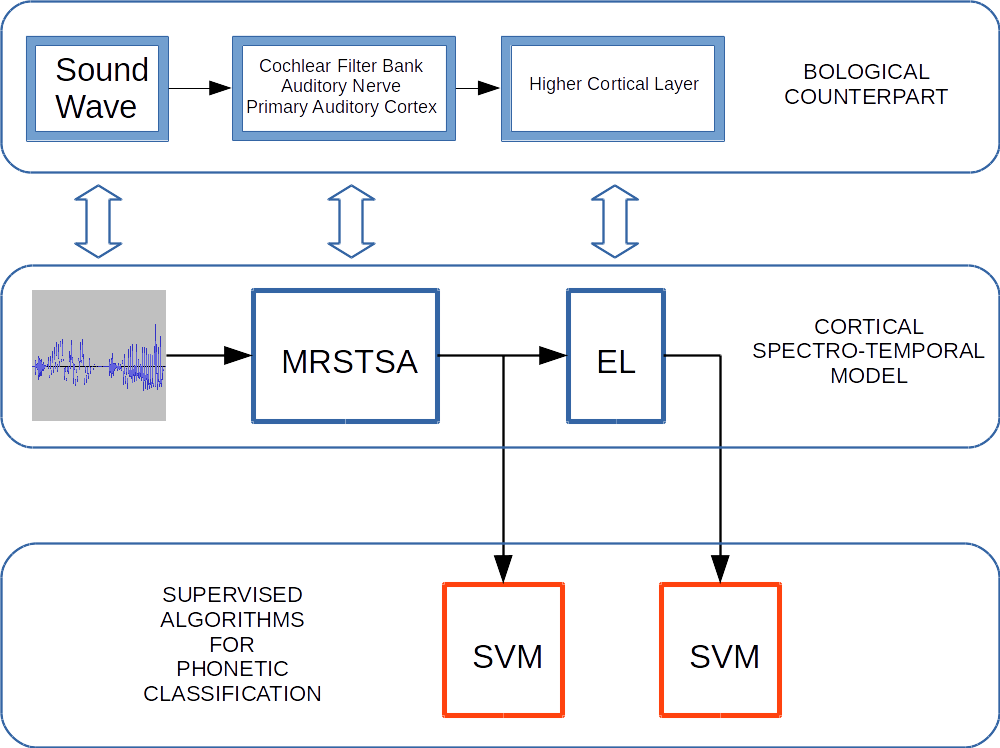
\includegraphics[width=0.8\textwidth]{Experiment.png}
    \caption{Experimental setup to test word classification task performances.
    Sound waves are processed by the \gls{mrstsa} algorithm.
    The outputs from the \gls{mrstsa} are processed by the \gls{el}.
    Word classification tasks are performed on both outputs by the \gls{svm} algorithm.
    Each section in the \gls{cstm} has its biological counterpart.}
    \label{fig:Experiment}
\end{figure}

We demonstrate via a computational simulation that our implementation of the cortical model leverages the performance in word classification tasks under certain environmental conditions (e.g., white noise and reverberation) and for certain variances applied to the auditory stimuli (e.g., pitch variations). We also demonstrate effectiveness in classifying multisyllabic words, which suggests that our implementation of neurophysiological predictive dynamics plus stochastic sparse patterns of activation outperforms the \gls{mrstsa} algorithm in terms of phonotactic sequential invariance for disturbances applied to the audio signal. 

Given these promising results, we posit that neurophysiological and anatomical properties in our model are potentially relevant to the design of artificial intelligence systems and may achieve higher levels of phonetic invariance and generalization than the ones achieved by current deep learning architectures.












\section*{Computational Model}

We introduce a computational model called \textbf{\glsfirst{cstm}}. The \gls{cstm} consists of two parts: The \glsfirst{el} and the \glsfirst{mrstsa}. 

The \glsfirst{el} converts a multidimensional array of real numbers into a multidimensional \gls{sdr}.
This stage is composed by a set of \glspl{som} \cite{kohonen_2082, Kohonen:1989:SAM:69371}
and incorporates neurophysiological phenomena such as columnar organization, afferent spontaneous
micro-columnar formation, proximal and distal dendritic arborization, lateral intercolumn interaction by means of independent dendritic \gls{nmda} branch activations, \glspl{mfe} with contextual stimulus adaptation, proximal lateral intracolumn inhibition, \gls{ltp}, \gls{ltd}, \gls{stdp} and distal synaptic homeostatic regulations.

% Finally, 

The algorithm, \glsfirst{mrstsa}, processes the sound waves to feed inputs to the \gls{el}, a technique that is inspired by Chi T. et al. \cite{chi_2005}.
In our \gls{mrstsa} implementation, we follow main guidelines from the higher cortical representations
developed in \cite{chi_2005}.


% GKT Note: I reworked the following into the above. 
%In order to obtain the inputs 
%with which 
%to feed the encoder,
%we implemented an algorithm called \glsfirst{mrstsa}.
%We process the sound waves with such algorithm
%that takes guidelines from
%the technique elaborated 
%which is inspired 
%by Chi T. et al. \cite{chi_2005}
%In such work, accumulating experimental findings
%from the central auditory system
%were exploited demonstrating its applications in the objective
%evaluation of speech intelligibility.
%As the authors pointed out, the model was not biophysical in spirit,
%but rather it abstracted from the physiological data an interpretation
%which was likely to be relevant in the design of sound engineering systems.

\subsection*{\glsfirst{el}}

The \gls{el} is responsible for generating \glspl{sdr} from the inputs delivered by the \gls{mrstsa} stage
described in section \nameref{sec-mrstsa} and from the activation history in its own \glspl{cc}.

The \gls{el} simulates a patch of cortical tissue called \gls{cl}using an n-dimensional array of complex structures called \glspl{csom} that simulate \glspl{cc} in the brain.

Each \gls{cc} in the \gls{el} is connected to the \gls{mrstsa} below by means of afferent connections. It is also
connected to neighboring \glspl{cc}--including possibly itself--in the \gls{el} by means of lateral connections and
to \glspl{cc} from other \glspl{cl} above by means of apical connections. Such connection scheme is shown in Fig \ref{fig:EncoderColumnConnections}.

\begin{figure}[h!]
    \centering
    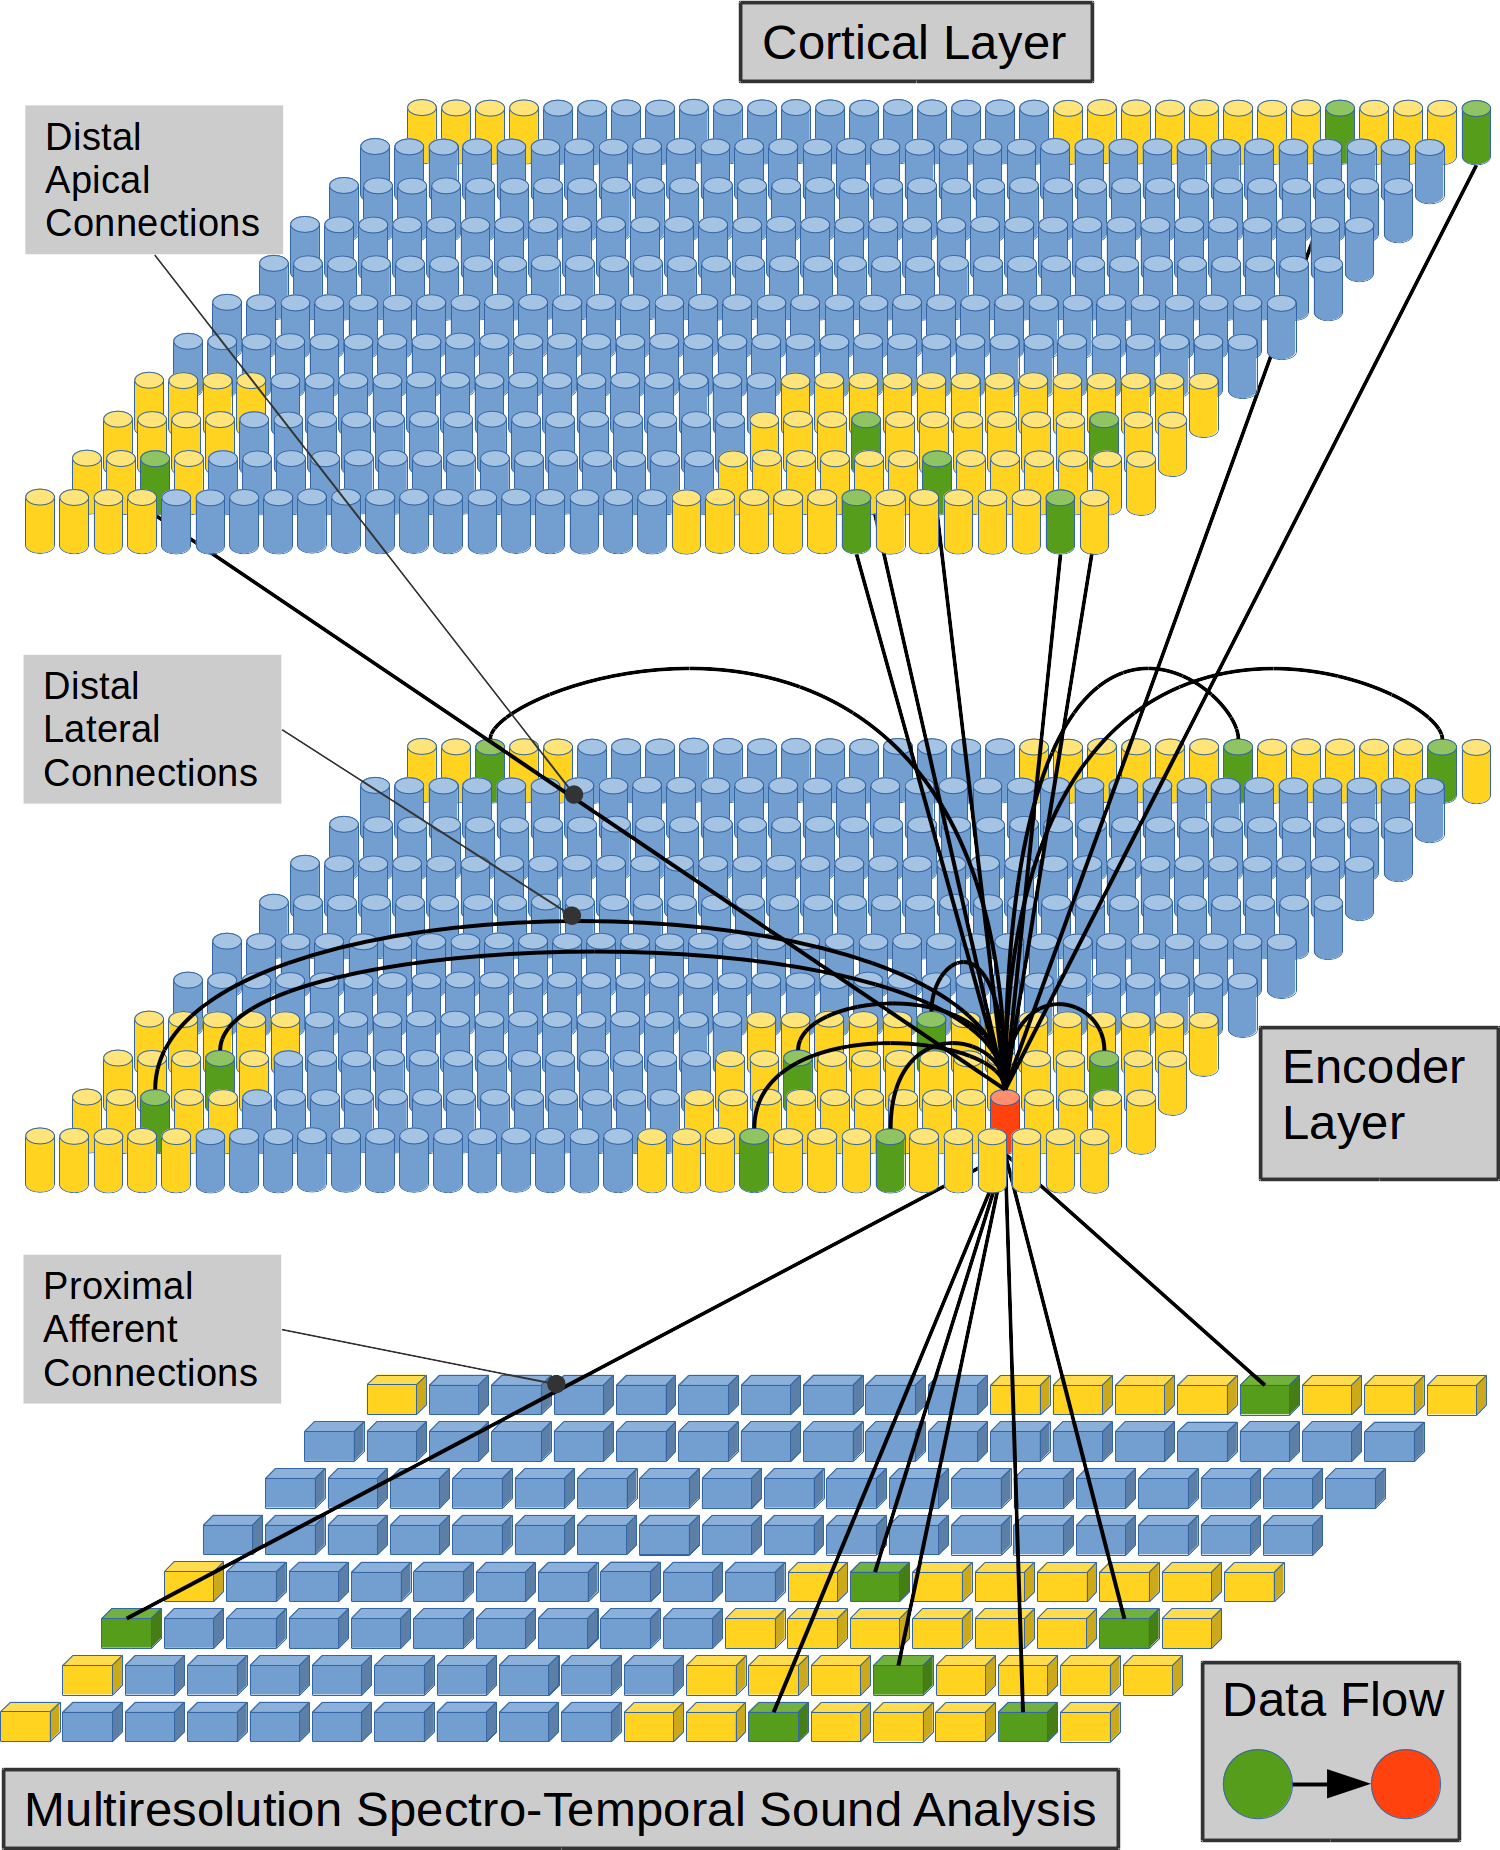
\includegraphics[width=0.6\textwidth]{EncoderColumnConnections.png}
    \caption{Connection scheme for a cortical column in the Encoder Layer.
	    Each cylinder in the \gls{el} and in the \gls{cl} represents a \gls{cc} in neural tissue.
	    Each prism in the \gls{mrstsa} represents a real valued variable.
	    This is a visualization of a \gls{cc} (in red) and its three receptive fields (in yellow).
	    The receptive field of a \gls{cc} is an array that defines a set of \glspl{cc}
	    with which such column could be connected.
	    The receptive field of a \gls{cc} on the \gls{mrstsa} determines an array of real valued variables
	    with which such column could be connected.
    A subset of \glspl{cc} in a receptive field (in green) represents the \glspl{cc} that are really
    connected with the \gls{cc} in red. A similar scenario could be described for the green prisms on
    the \gls{mrstsa}.
    The size, wrap-around property and percentage of established links (in green) inside a receptive field are tunable parameters for the model.
    In this work, only lateral connections have been implemented since in the current implementation there are no upper cortical layers from which
    to bring apical connections.}
    %Every neural unit in a \gls{cc} in the \gls{el} receives the same set of proximal connections from
    %the \gls{mrstsa}.
    %Such connections are modified following the statistical distribution from the \gls{mrstsa}
    %by means of the \gls{som} algorithm.}
    \label{fig:EncoderColumnConnections}
\end{figure}


\iffalse
\begin{figure}[h!]
    \centering
    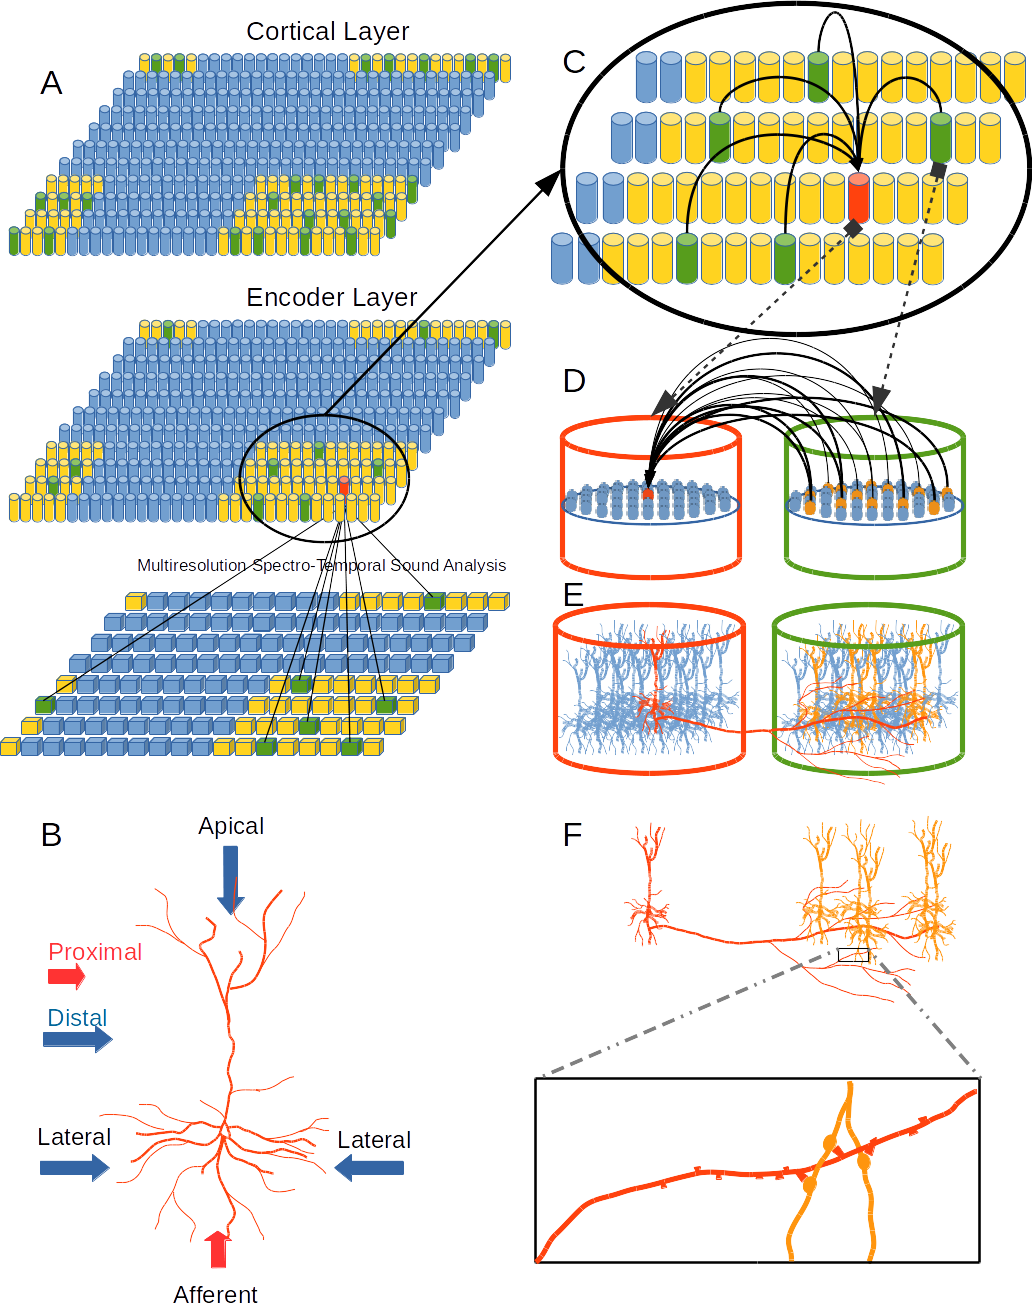
\includegraphics[width=0.9\textwidth]{Connectivity.png}
    \caption{\tiny Connection scheme for a cortical column in the Encoder Layer.
	    (A) Each cylinder in the \gls{el} and in the \gls{cl} represents a \gls{cc} in neural tissue.
	    Each prism in the \gls{mrstsa} represents a real valued variable.
	    This is a visualization of a \gls{cc} (in red) and its three receptive fields (in yellow).
	    The receptive field of a \gls{cc} is an array that defines a set of \glspl{cc}
	    with which such column could be connected.
	    The receptive field of a \gls{cc} on the \gls{mrstsa} determines an array of real valued variables
	    with which such column could be connected.
    A subset of \glspl{cc} in a receptive field (in green) represents the \glspl{cc} that are really
    connected with the \gls{cc} in red. A similar scenario could be described for the green prisms on
    the \gls{mrstsa}.
    The size, wrap-around property and percentage of established links (in green) inside a receptive field are tunable parameters for the model.
    Every neural unit in a \gls{cc} in the \gls{el} receives the same set of proximal connections from
    the \gls{mrstsa}.
    Such connections are modified following the statistical distribution from the \gls{mrstsa}
    by means of the \gls{som} algorithm.
    (B) Connectivity profile of a pyramidal neural unit in the \gls{el}.
    Proximal connections are formed only by afferent connections from the \gls{mrstsa}
    while distal connections are formed by lateral and apical connections from neighboring columns and
    from columns in another cortical layer above respectively.
    (C) Distal dendritic branches from neighboring \glspl{cc} inside the receptive field
    of a \gls{cc} in the \gls{el}. A distal dendritic branch between the red \gls{cc} and a
    green \gls{cc} means that every neural unit in the red \gls{cc} is linked with a different
    subset of neural units in the green \gls{cc} by means of potential connections.
    (D) Potential connections in a dendritic branch which link a neural unit in the red \gls{cc}
    with a subset of neural units in a green \gls{cc}. The subset of potential connections comes from a percentage of neural units
    inside the green \gls{cc}. Such percentage is a tunable parameter for the \gls{cc}.
    (E) A distal dendritic branch between a pyramidal cell in a \gls{cc} and a 
    sub-set of pyramidal cells in a neighboring \gls{cc} inside its receptive field
    in the \gls{el}.
    (F) Physical proximity of a dendritic branch from the red cell to axonal branches from yellow cells constitutes potential connections
    which could prosper becoming in established synapses depending on the sequential activity among cells.}
    \label{fig:Connectivity}
\end{figure}
\fi

Both lateral and apical are feedback connections that constitute contextual information channels. 
These channels put the current afferent excitation under the context of previous activations.
Such connections damp the activity of some units allowing only the precise activations
of specific neural units in an afferently excited \gls{cc}.
Such precise activations match the sequential paradigms learned by the network.

Recent findings in neuroscience \cite{Marques2018} support the idea 
that feedback could potentially enhance visual representations in time and space
damping the activity of certain cells while allowing the activations  of others
which agree with its predictions.

In this paper we only implement lateral connections since
there are no upper layers 
from which to bring apical information in the present implementation.

Each cell unit in a \gls{cc} has two types of dendritic branches; proximal and distal.
Proximal and distal dendritic branches lead to proximal and distal connections in a cell unit respectively.
Proximal and distal connections produce different effects on a neural unit's plasticity and activation.
Neural units in the \gls{el} simulates pyramidal cells in cortical tissue in the brain.
Fig \ref{fig:PyramidalCell} shows the connectivity profile in such units. 

\begin{figure}[h!]
    \centering
    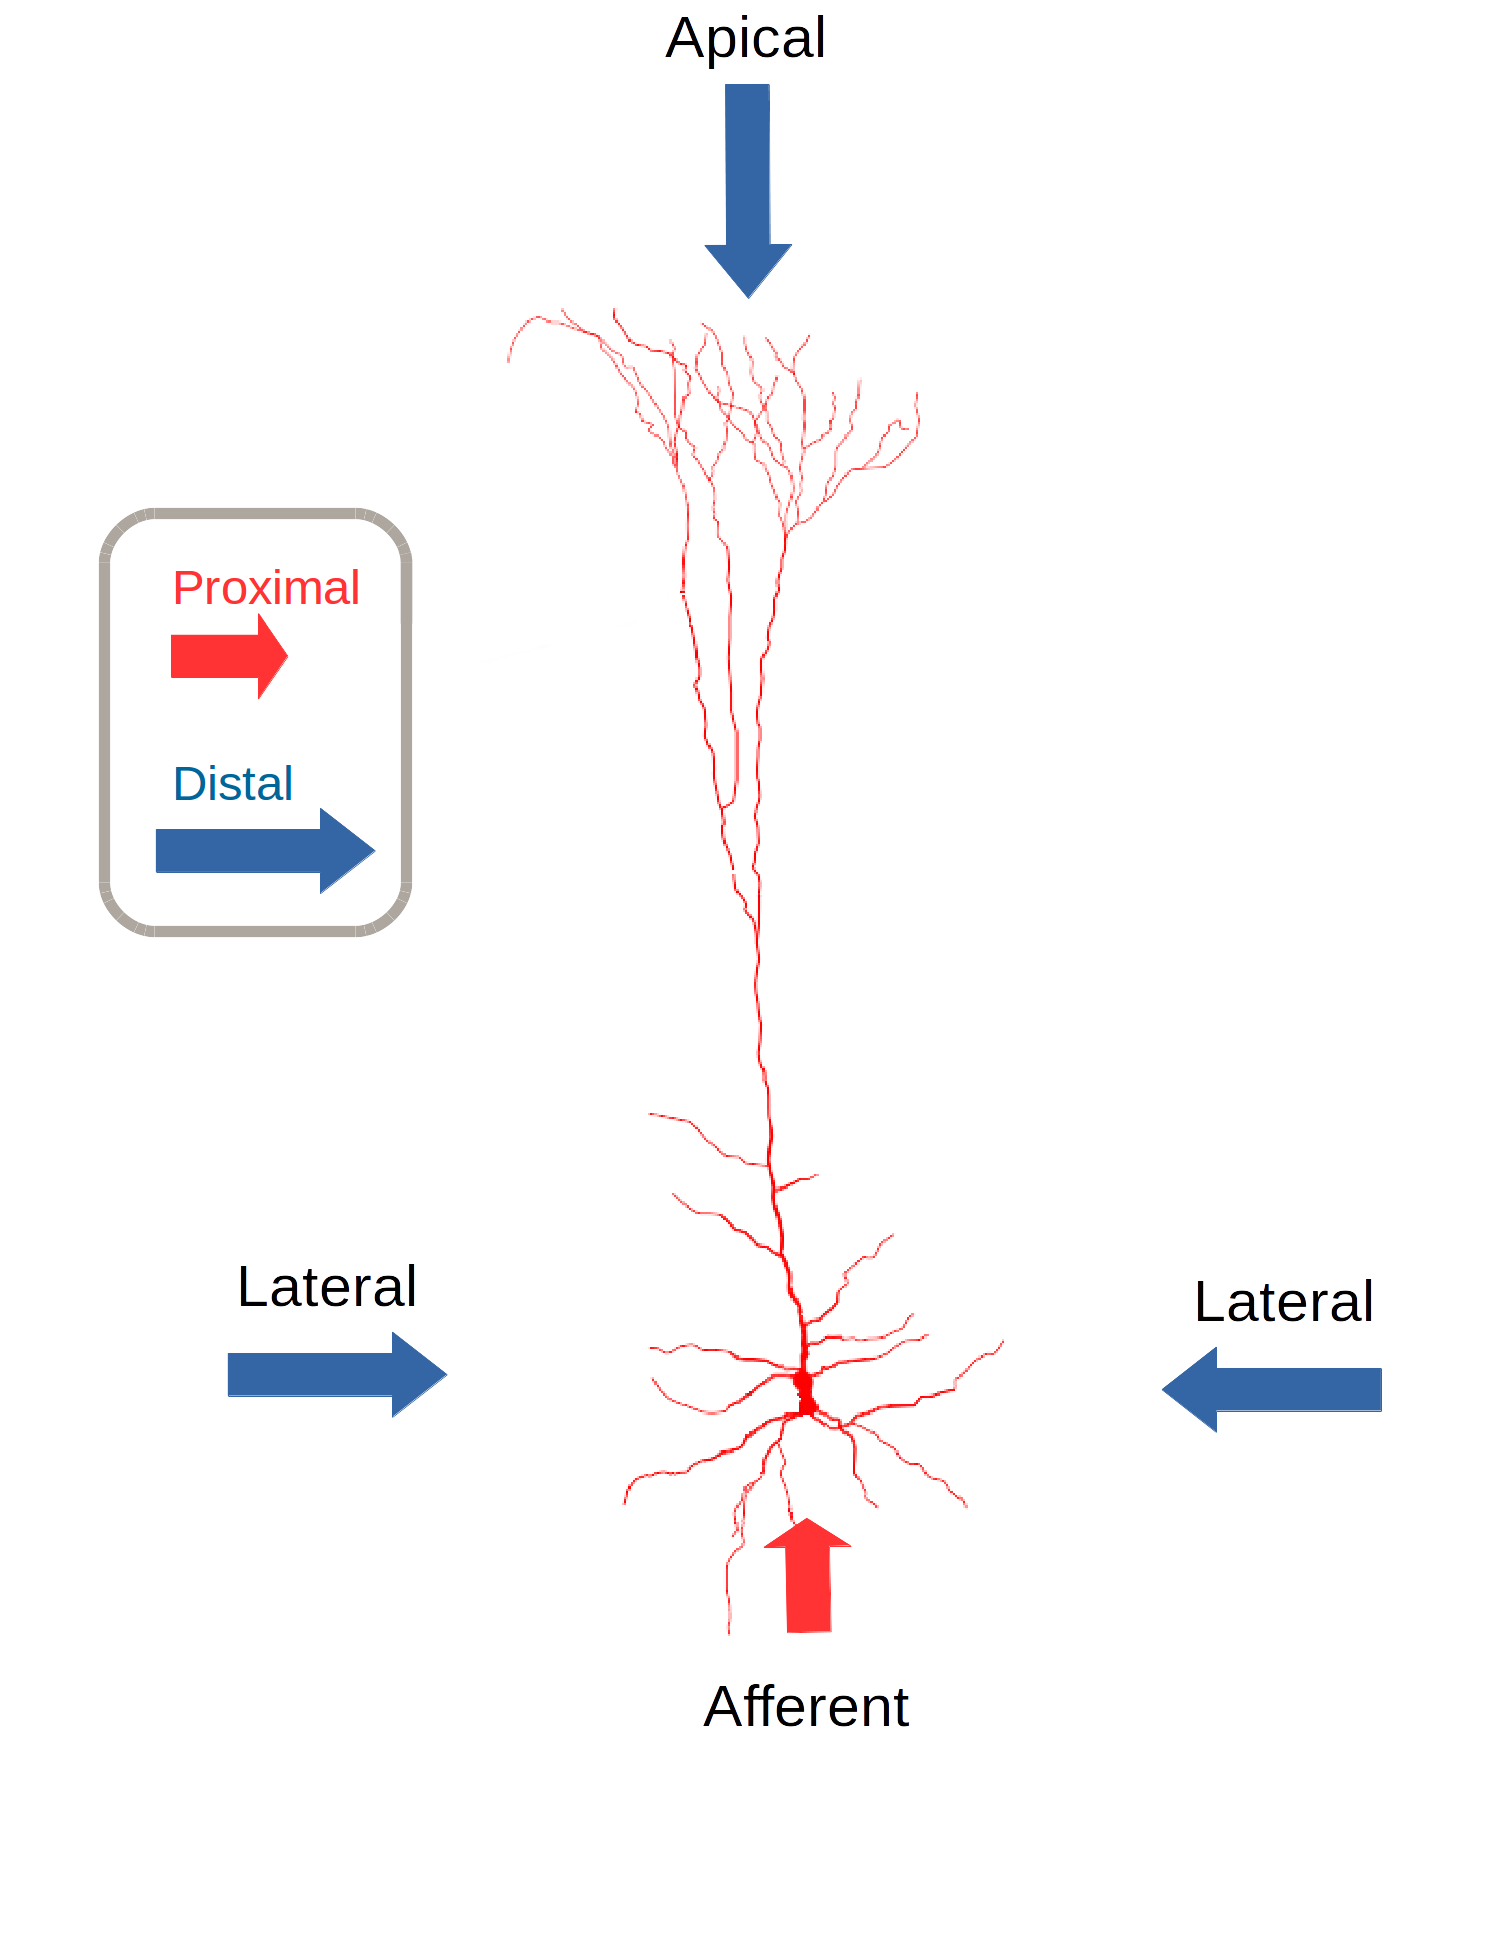
\includegraphics[width=0.9\textwidth]{PyramidalCell.png}
    \caption{Connectivity profile of a pyramidal neural unit in the \gls{el}.
    Proximal connections are formed only by afferent connections from the \gls{mrstsa}
    while distal connections are formed by lateral and apical connections from neighboring columns and
    from columns in another cortical layer above respectively.
    Adapted from 
    (Fabuio - Own work, CC BY 4.0, \url{https://commons.wikimedia.org/w/index.php?curid=60707501)}}
    \label{fig:PyramidalCell}
\end{figure}

\subsubsection*{Proximal dendritic connections}

In reference to proximal connections in the \gls{el}, each neural unit in a \gls{cc} has the same set of
proximal connections to the \gls{mrstsa} (Fig \ref{fig:EncoderColumnConnections}).
Such connections constitute a multidimensional space of real numbers.
In order to acquire the statistical distribution in such multidimensional real space we use
a multidimensional \gls{som} in each cortical column.

A \gls{som} is an unsupervised clustering algorithm which distributes a continuous multidimensional distribution
in a discrete multidimensional distribution of units \cite{Kohonen:1989:SAM:69371, kohonen_2082}.
In this way we ended up with an array of units of $m$ dimensions in which each unit
represents a set of vectors from the continuous distribution in an input space of $n$ dimensions.
Generally, $m < n$ in order to reduce the dimensionality in the discrete representation.
We added such restriction in our columnar algorithm.

In the \gls{som} algorithm, each input vector has to be completely determined.
In our case, some inputs from the \gls{mrstsa} could be null,
and each input vector could not have the information of each of its components available.
We incorporated a stochastic mechanism in the \gls{el} in order to deal with such situation.
We made each afferent connection to learn statistical boundaries from its corresponding input.
We establish a minimum-maximum margin in each proximal connection in the \gls{el}.
Such margin is consistent with the statistical distribution in the history of its corresponding input.
When an afferent input is undetermined, in a context in which some afferent inputs have
available information,
the \gls{el} chooses
the value in the undetermined input
%is chosen
randomly
between the boundaries learned for such input.

We call our implementation of the \gls{som} algorithm, \gls{ssom}.
The \gls{ssom} algorithm accounts for proximal lateral intra-column interaction, \gls{ltp} and
\gls{ltd}.
It also dissociates proximal dendritic inputs from distal dendrites, since
it modifies
proximal connections
%are modified
following the statistical distribution from the
\gls{mrstsa} independently of the units that fire in such \gls{cc}.
This independence in the plasticity of the proximal dendritic inputs
%uses
is supported by
the
%fact
property
found in cortical tissue by means of which there is dendritic plasticity
in the context of partial depolarization of the soma \cite{reiter_1998}--that is, without an \gls{ap}. % Citation needed here

The term \textit{static} comes from the fact that the patterns learned from proximal afferent
dendrites do not account for the contextual history in the dynamic evolution
of the algorithm.








\subsubsection*{Distal dendritic connections}

In terms of distal dendritic branches, each \gls{cc} in the \gls{el} is connected to other \glspl{cc}--in green in Fig \ref{fig:EncoderColumnConnections}--by means of such
branches inside the receptive fields--in yellow in Fig. \ref{fig:EncoderColumnConnections}--from the same \gls{el} and from another \gls{cl}
above.
Each link between the red \gls{cc} and a green \gls{cc}--Fig. \ref{fig:DistalDendrites} A--
symbolizes the fact that each cell unit in
the red \gls{cc} is linked with a different subset of cell units in the green \gls{cc}--Fig. \ref{fig:DistalDendrites} B.

\begin{figure}[h!]
    \centering
    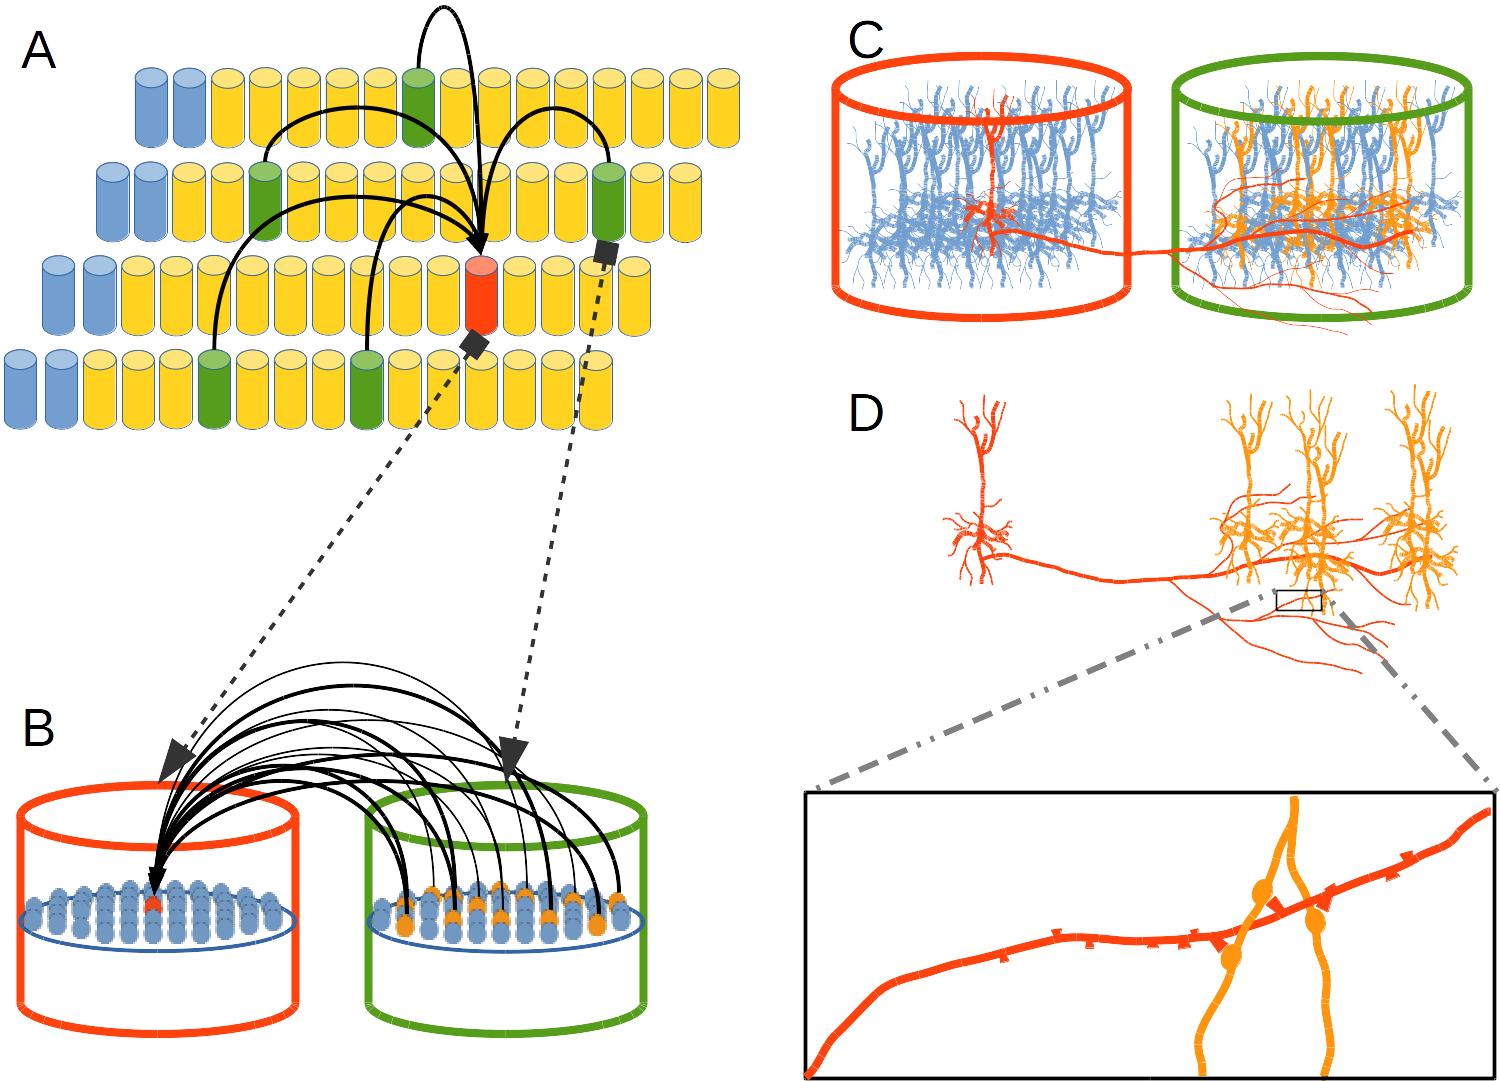
\includegraphics[width=0.9\textwidth]{DistalDendrites.png}
    \caption{Distal dendrite connections. (A) Distal dendritic branches from neighboring \glspl{cc} inside the receptive field
    of a \gls{cc} in the \gls{el}. A distal dendritic branch between the red \gls{cc} and a
    green \gls{cc} means that every neural unit in the red \gls{cc} is linked with a different
    subset of neural units in the green \gls{cc} by means of potential connections.
    (B) Potential connections in a dendritic branch which link a neural unit in the red \gls{cc}
    with a subset of neural units in a green \gls{cc}. The subset of potential connections comes from a percentage of neural units
    inside the green \gls{cc}. Such percentage is a tunable parameter for the \gls{cc}.
    (C) A distal dendritic branch between a pyramidal cell in a \gls{cc} and a 
    sub-set of pyramidal cells in a neighboring \gls{cc} inside its receptive field
    in the \gls{el}.
    (D) Physical proximity of a dendritic branch from the red cell to axonal branches from yellow cells constitutes potential connections
    which could prosper becoming in established synapses depending on the sequential activity among cells.}
    \label{fig:DistalDendrites}
\end{figure}

Such links in Fig \ref{fig:DistalDendrites} A, represent dendritic branches in neural tissue and
we call
each connection in Fig. \ref{fig:DistalDendrites} B,
%is called
potential connection.
%and
Potential connections represent synapses in the dendritic branch.
A cell unit inside the red \gls{cc} ends up with as many dendritic branches as green \glspl{cc} inside its receptive field (Fig \ref{fig:DistalDendrites} A.)

The term \emph{potential connection} is used, because it describes a pair of neural units linked by its physical location and dendritic and axonal disposition in cortical tissue (Fig. \ref{fig:DistalDendrites} C). However, an effective connectivity between such neurons will depend upon their sequential pattern of activation which will establish developed synapses between them. If two neural units--a red one and a yellow one in Fig. \ref{fig:DistalDendrites} D--are linked by means of a distal potential connection--produced by a synapse between a distal dendritic branch from the red one and an axonal branch from the yellow one--such connection will grow only if there is a sequential activation of the red cell after an activation of the yellow cell, in two consecutive time steps. If such phenomenon does not repeat itself over time, such synapse will decrease its strength with respect to other synapses in the dendritic branch in the red cell in Fig. \ref{fig:DistalDendrites} D. A simultaneous activation in both neural units--the red one and the yellow one in Fig. \ref{fig:DistalDendrites} D--will decrease the strength in such potential connection.

We implemented distal dendritic synaptic plasticity mechanisms by means of an algorithm called \gls{dsom}.
The learning mechanisms implemented on such algorithm simulate neurophysiological phenomena
such as \gls{stdp}, and homeostatic regulation plasticity in the synaptic strength regulation in
distal dendritic branches.







\subsubsection*{Activation rules in a \gls{cc}}

Finally, in reference to the activation rules of neural units inside a \gls{cc} in the \gls{el},
first a group of cell units in a \gls{cc} is partially depolarized 
by distal connections among such neural units and cell units activated in the
previous time step in the \gls{el}--Fig. \ref{fig:Activation} A.
That is, neural units activated in time step $t=0$ in the \gls{el}, will partially depolarize
a set of neural units in time step $t=1$ in such \gls{cc}, by means of distal--lateral and apical--
dendritic branch synapses established by learning in the \gls{dsom} algorithm.

Second, afferent proximal connections from \gls{mrstsa} will tend to depolarize
certain clusters of units in such \gls{cc} in time step $t=1$--Fig. \ref{fig:Activation} B.
The tentative depolarization is produced by the inputs from the \gls{mrstsa} with
proximal synapses established by learning in the \gls{ssom} algorithm. 
Such group of neural units are randomly chosen from a discrete distribution
whose probabilities are established by the state of excitation in afferent inputs.

If a sufficient number of partially depolarized units are in the set of
afferently excited units, such partially depolarized units
will fire previously in the group--Fig. \ref{fig:Activation} B left.
Those units--which fire before--prevent neighboring units in the excited clusters from firing,
hyperpolarizing them by means of lateral inhibitory connections in the column.

\begin{figure}[h!]
    \centering
    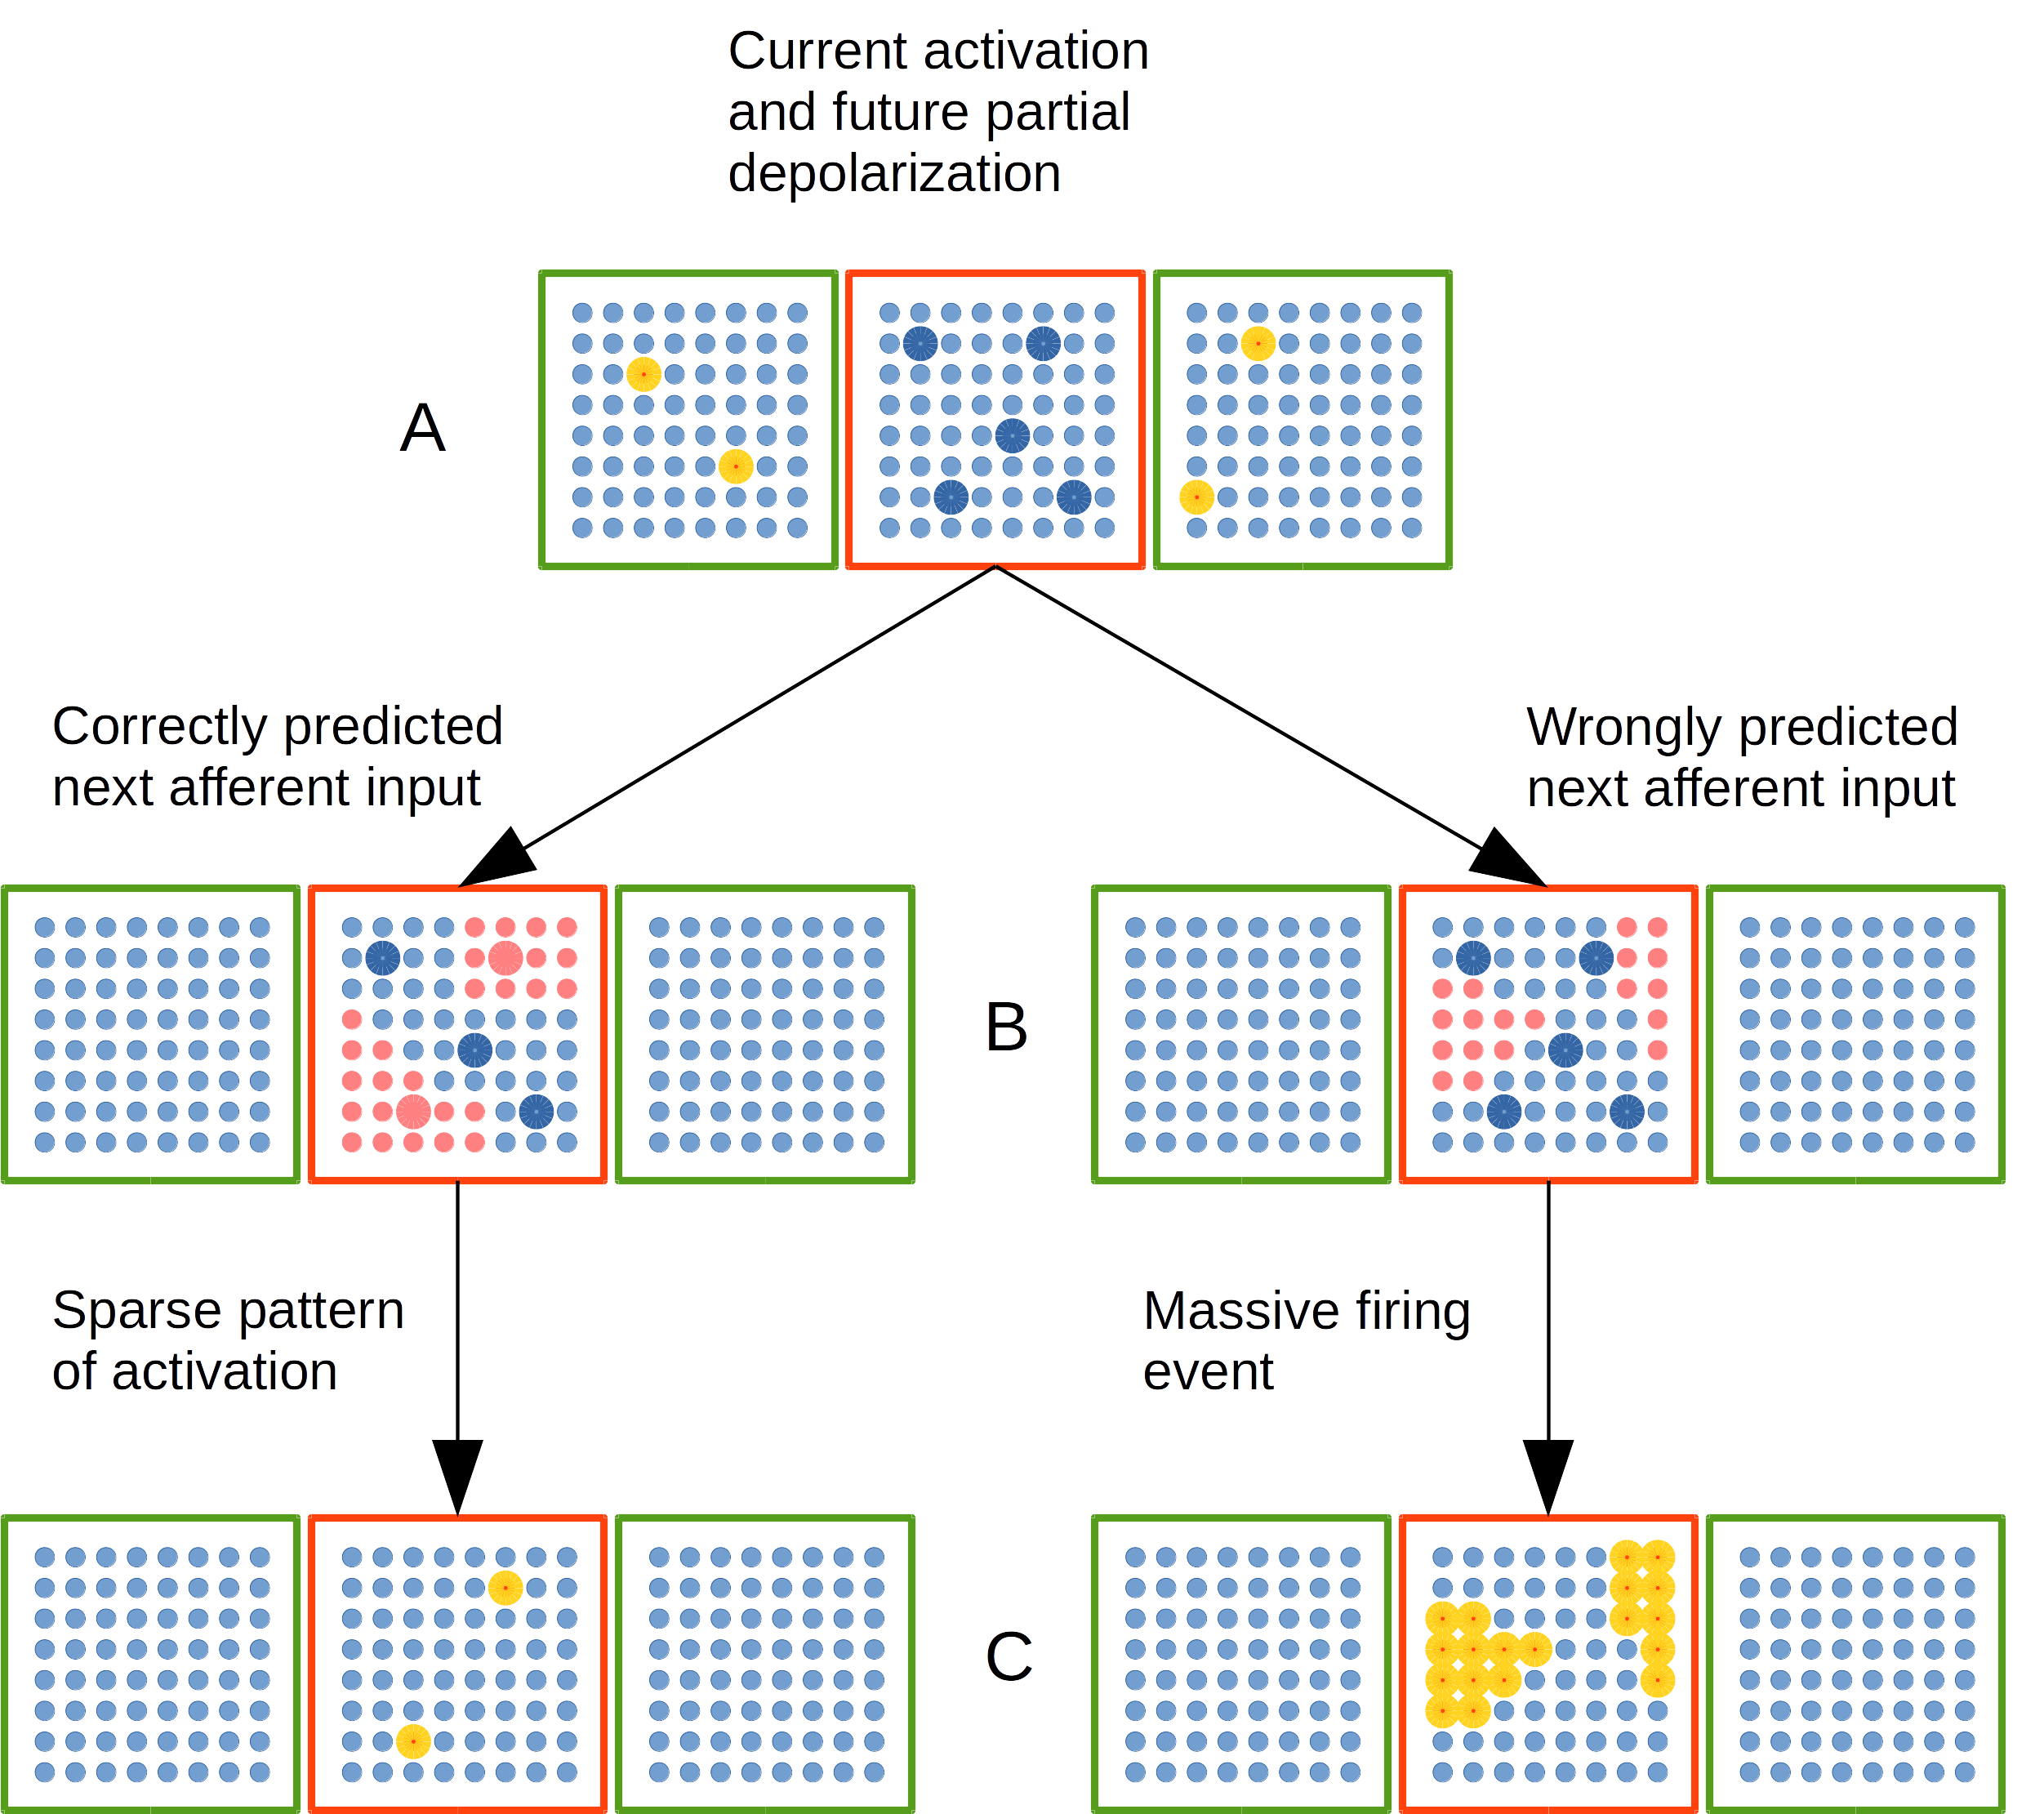
\includegraphics[width=0.7\textwidth]{Activation.png}
    \caption{Dynamic cellular activation in a \gls{cc} in the \gls{el}.
    A red cortical column is linked with two green cortical columns by means of distal dendrites.
    (A) Cellular activation in green \glspl{cc}--highlighted yellow cells--puts neural units
    in red \gls{cc} in a partially depolarized--predictive state highlighted in blue.
    (B) Cluster of neural cells activated by afferent inputs.
    Left: A substantial amount of partially depolarized cells are in the afferently excited cellular clusters.
    Right: There is no substantial amount of partially depolarized cells inside afferently excited cellular clusters.
    (C) \gls{cc} with active cellular units highlighted in yellow.
    Left: Sparse pattern of cellular activation.
    Right: Massive pattern of activation.}
    \label{fig:Activation}
\end{figure}

Partial depolarization states put cell units in a predictive state generated by
the activations produced in the \gls{el} in previous time steps.
That is, lateral and apical activation in previous time steps constitutes a context in which
current afferent inputs are received.

From the group of units that tend to be depolarized by current afferent inputs from the \gls{mrstsa},
only a reduced sub-set of those units are likely to fire in the previous contextual firing history
in the \gls{el}--Fig. \ref{fig:Activation} C left.

In case there is no context, that is, none of the units which tend to be depolarized by afferent inputs
is partially depolarized by previous--lateral and apical--activations--Fig. \ref{fig:Activation} B right--,
all units in the afferent excited clusters will be active, covering more hypotheses for next inputs--Fig. \ref{fig:Activation} C right.

Each neural unit in a \gls{cc} establishes its state of partial depolarization based on the contribution from
distal dendritic branches from lateral and apical connections.
A dendritic branch will contribute to the partial depolarization of the soma in such cell only if such
dendritic branch exceeds an activation threshold by means of the contribution from its individual synapses
in the context of the patterns of activation in the previous time step.

This mechanism has compelling sequential properties \cite{hawkins_2016},
which have already been applied in the classification of artificially generated sequential data \cite{cui_2016}.
We apply such mechanism in the \gls{dsom} algorithm by adding the contribution of synapses--in a dendritic branch--
whose connections are linked with cells that were active in the previous time step in the \gls{el}.

















\subsection*{\glsfirst{mrstsa}}
\label{sec-mrstsa}

In Chi T. et al. \cite{chi_2005}, a computational model of auditory analysis is described.
The model is inspired by psychoacoustical and
neurophysiological findings in early and central stages of the auditory system.
Such model provided
an unified multiresolution representation of the spectral and temporal features
which were interpreted as critical for the perception of sound.

The original algorithm has a subcortical and a cortical stage.
For the subcortical stage, first an affine wavelet transform of the acoustic signal
represents the spectral analysis performed by the cochlear filter bank.
Second, the cochlear filter outputs are transduced into auditory-nerve
patterns by a hair cell stage consisting of a high-pass filter,
a nonlinear compression and a membrane leakage low-pass filter.
Third, a first-order derivative with respect to the tonotopic axis
followed by a half-wave rectifier
simulates the action of a lateral inhibitory
network postulated to exist in the cochlear nucleus,
which effectively enhances the frequency
selectivity of the cochlear filter bank.
The final output of this stage is obtained by integrating
over a short window, with time constant of 8 ms, mimicking
the further loss of phase locking observed
in the midbrain.

The cortical stage mimics aspects of the responses of higher
central auditory stages, especially \gls{a1}.
Functionally, this stage estimates the
spectral and temporal modulation content of the auditory
spectrogram. It does so computationally via a bank of filters
that are selective to different spectrotemporal modulation parameters
that range from slow to fast rates temporally, and
from narrow to broad scales spectrally. The \glspl{strf}
of these filters are also centered at
different frequencies along the tonotopic axis.

Since we prompt a parsimonious incorporation of neurophysiological
properties--mainly centered in cortical features--
we followed the main guidelines in the implementation of the cortical section of such model. 
We implemented the initial stage in our model with the application of \gls{fft} to the audio vector
with a different sample window for each resolution.
We then extracted the power spectral density from each resolution.
In this way we obtained a multiresolution spectral analysis of the audio signal,
with high spectral and low temporal resolution for wider sample windows and
vice versa.
Such different time windows in the \gls{fft},
incorporated--at the same time--leakage low-pass filters with a time constant for each
resolution accounting for decrease of phase-locking in the auditory nerve.
We then applied a \gls{mfb} with 128 elements to each spectrum
in order to represent the spectral analysis performed by the cochlear filter bank.
Then, we convolved each resolution obtained in the last step along its tonotopic axis
with a complex multiresolution function whose real part
was a symmetric Mexican hat function and its imaginary part was its antisymmetric Hilbert transform.
With this strategy we incorporated the phenomena of symmetry \cite{shamma_1993}, bandwidth \cite{schreiner_1990}
and frequency modulation selectivity \cite{shamma_1993,heil_1992,mendelson_1985}
found in \gls{a1} and incorporated in the original algorithms \cite{wang_1995}.

We obtained the magnitude of each convolution and applied normalization to each time window
as a mean of automatic gain control in order to prioritize the information delivered by the
spectral configuration and not the absolute values delivered by the filters. 

By means of this constraint we account for the mechanical and chemical properties of hair cells in the mammalian inner ear
which constitute a transduction mechanism that appears to adapt to recent stimulus history in a way that can affect its gain
\cite{eatock_2000,holt_2000,le_goff_2005}. 
We decided to be conservative, not including
sound intensity dimension but just the shape of the filter responses.
























%\section{Phonetic Classification, a Case Study}

%We propose a computational approach called \gls{cstm}, which consists of two parts: The \gls{el} and the \gls{mrstsa}.  

%The algorithm \gls{mrstsa}, which processes the sound waves to feed inputs to the \gls{el}, is a technique inspired by Chi T. et al. \cite{chi_2005}. In their work, accumulating experimental findings from the central auditory system were exploited demonstrating its applications in the objective evaluation of speech intelligibility. In the present work, since we prompt a parsimonious incorporation of neurophysiological properties--mainly centered in cortical features--we followed the main guidelines in the implementation of the cortical section of such model.

%The \gls{el} converts a multidimensional array of real numbers into a multidimensional \gls{sdr}. This stage is composed by a set of \glspl{som} \cite{kohonen_2082, Kohonen:1989:SAM:69371} and incorporates neurophysiological phenomena such as columnar organization, afferent spontaneous micro-columnar formation, proximal and distal dendritic arborization, lateral intercolumn interaction by means of independent dendritic \gls{nmda} branch activations, \glspl{mfe} with contextual stimulus adaptation, proximal lateral intracolumn inhibition, \gls{ltp}, \gls{ltd}, \gls{stdp} and distal synaptic homeostatic regulations.

%In the present work, we studied the level of invariance in the phonetic features abstracted by the \gls{el}, by means of comparing such representations with the multiresolution spectro-temporal auditory features returned by the \gls{mrstsa} algorithm. To this end, we evaluated the features returned by each algorithm in different word classification tasks. In order to asses the word classification performance in each algorithm, we used \gls{svm} technique with the experimental setup depicted in Fig. \ref{fig:Experiment}.

%\begin{figure}[h!]
    %\centering
    %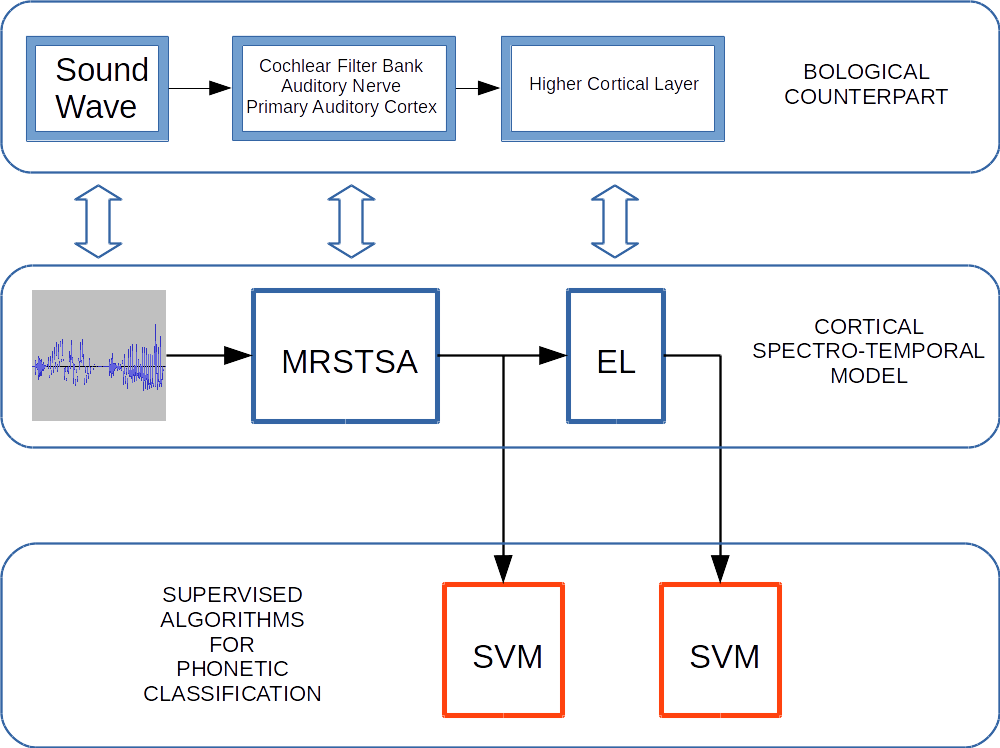
\includegraphics[width=0.5\textwidth]{Experiment.png}
    %\caption{Experimental setup to test word classification task performances.
    %Sound waves are processed by the \gls{mrstsa} algorithm.
    %The outputs from the \gls{mrstsa} are processed by the \gls{el}.
    %Word classification tasks are performed on both outputs by the \gls{svm} algorithm.
    %Each section in the \gls{cstm} has its biological counterpart.}
    %\label{fig:Experiment}
%\end{figure}

%In the experimental procedure we first trained the \gls{el} with an original corpus of 500 words from a vocabulary of 5 words with 10 different voices (8 males and 2 females) generated by \gls{festival} Synthesis \cite{festival2014} speech synthesizer. Afterwards, we processed the same corpus with the \gls{el} in inference mode. In such mode, the \gls{el} processed the information with its learning properties disabled. In this manner, during inference, the \gls{el} did not modify its synapses and just returned patterns of activation in response to the stimuli it received. We then used the outputs from the \gls{mrstsa} and the \gls{el} in inference mode to train the \gls{svm} classifiers. The cross validation training performances are shown in Table~\ref{SVM_Training}.

%\begin{table}[h!]
%\centering
%\caption{\gls{svm} 5-fold cross validation training results}
%\begin{tabular}{|l|l|l|}
%\hline
                   %& MRSTSA & Encoder Layer \\ \hline
%Monosyllabic Words & 98.8\% & 99\%          \\ \hline
%Disyllabic Words   & 98\%   & 97.8\%        \\ \hline
%Trisyllabic Words  & 97.6\% & 98\%          \\ \hline
%\end{tabular}
%\label{SVM_Training}
%\end{table}

%In a second stage, we ran the \gls{el} in inference mode again, but this time we affected the original corpus by means of different kind of variances. We tested the performances of the--already trained--classifiers in the presence of the features returned by the algorithms in response to the corpus affected by the variances which we introduced to original corpora by means of Audacity \cite{audacity}. The variances introduced to the original corpus included white noise, reverberation and pitch variations. The average classification performances are shown in Fig. \ref{fig:AV_ACC}.

%%The classification performances are shown in Figs. \ref{fig:MONO_ACC}, \ref{fig:DI_ACC} and \ref{fig:TRI_ACC}.

%%\begin{figure}[h!]
    %%\centering
    %%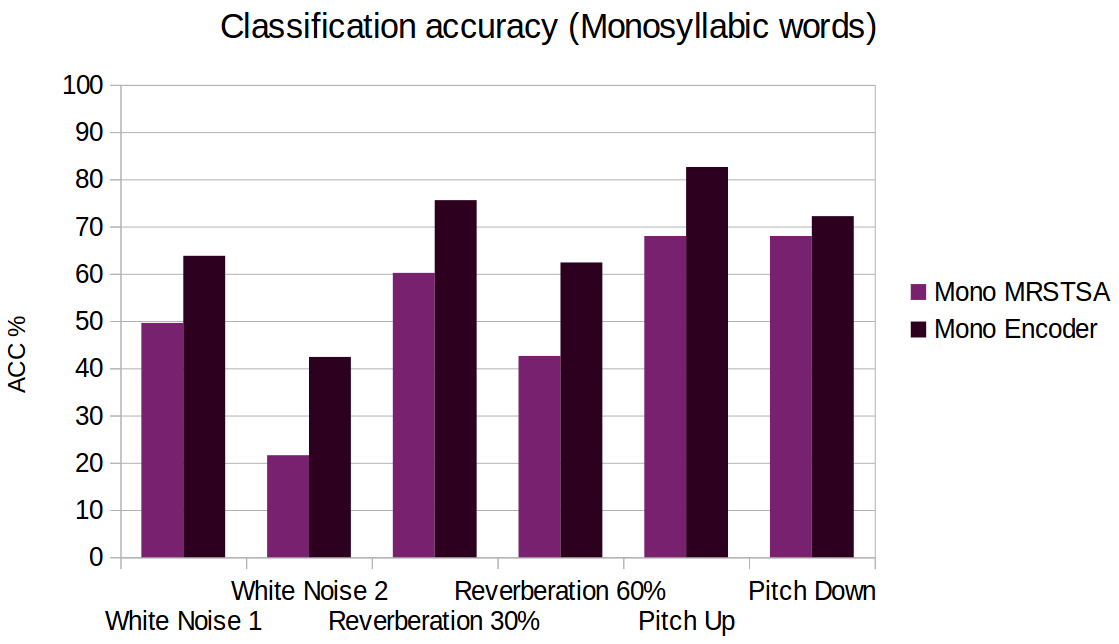
\includegraphics[width=0.9\textwidth]{MONO_ACC.png}
    %%\caption{\gls{mrstsa} and \gls{el} classification accuracies against different variances introduced to the original signals
    %%for \textbf{monosyllabic words}.
    %%White Noise 1 determines a \gls{snr} average \gls{rms} power rate of 19.8 dB while White Noise 2 13.8 dB.
    %%Reverberation 30\% determines a \gls{rt} value of 0.61 seconds while Reverberation 60\% determines a \gls{rt} value of 1.78 seconds.
    %%Pitch Up determines a pitch move from E to G, while Pitch Down determines a pitch move from E to C.}
    %%\label{fig:MONO_ACC}
%%\end{figure}

%%\begin{figure}[h!]
    %%\centering
    %%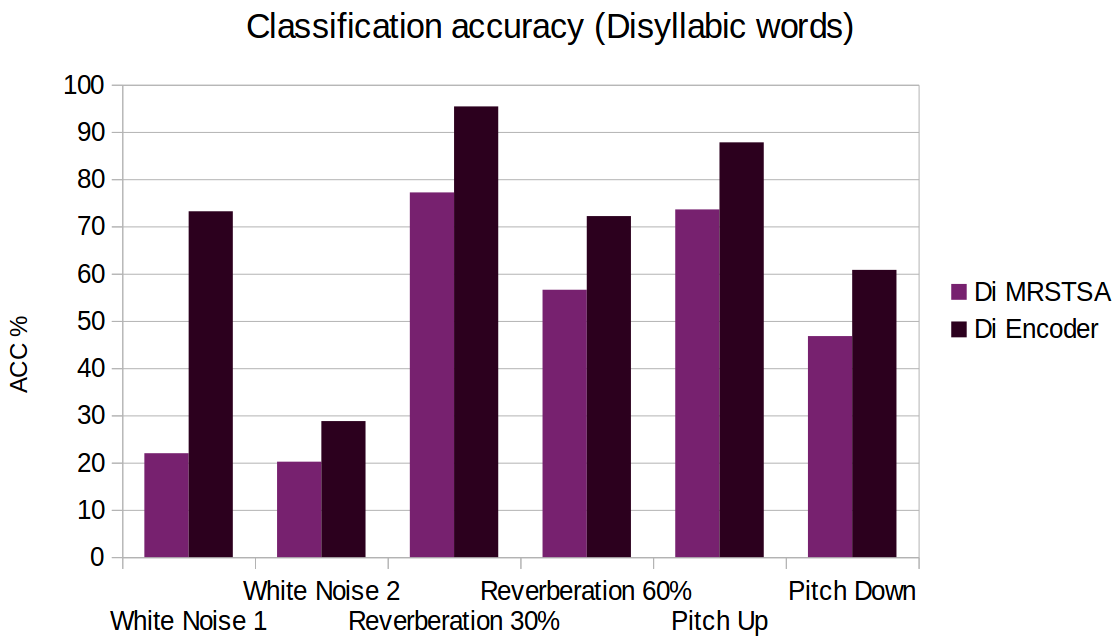
\includegraphics[width=0.9\textwidth]{DI_ACC.png}
    %%\caption{\gls{mrstsa} and \gls{el} classification accuracies against different variances introduced to the original signals
    %%for \textbf{disyllabic words}.
    %%White Noise 1 determines a \gls{snr} average \gls{rms} power rate of 19.8 dB while White Noise 2 13.8 dB.
    %%Reverberation 30\% determines a \gls{rt} value of 0.61 seconds while Reverberation 60\% determines a \gls{rt} value of 1.78 seconds.
    %%Pitch Up determines a pitch move from E to G, while Pitch Down determines a pitch move from E to C.}
    %%\label{fig:DI_ACC}
%%\end{figure}

%%\begin{figure}[h!]
    %%\centering
    %%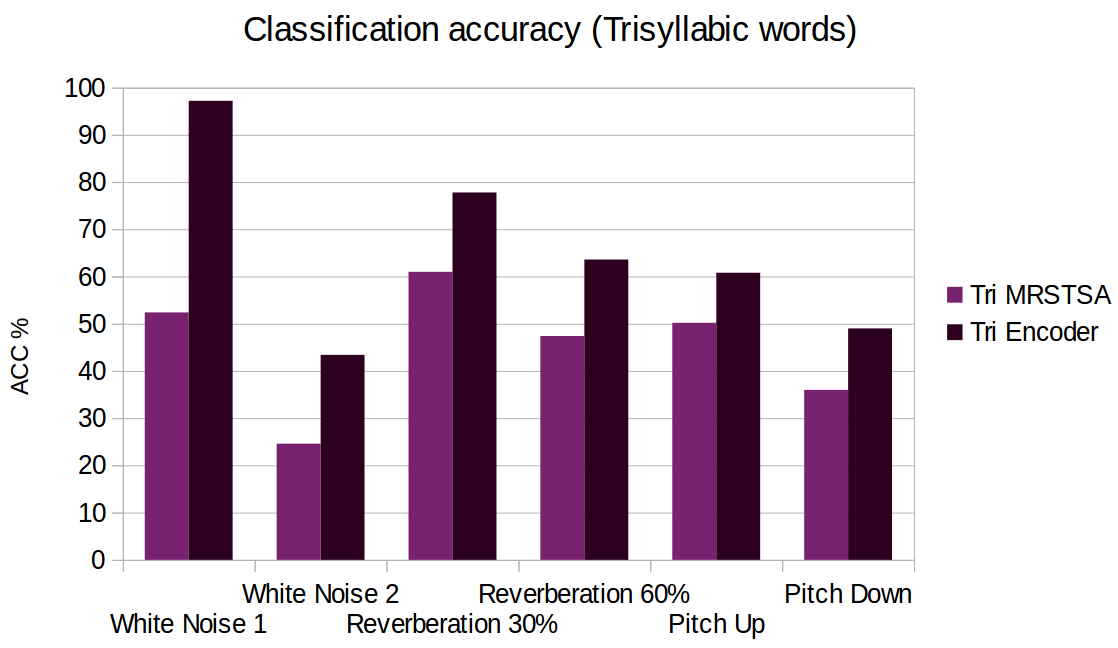
\includegraphics[width=0.9\textwidth]{TRI_ACC.png}
    %%\caption{\gls{mrstsa} and \gls{el} classification accuracies against different variances introduced to the original signals
    %%for \textbf{trisyllabic words}.
    %%White Noise 1 determines a \gls{snr} average \gls{rms} power rate of 19.8 dB while White Noise 2 13.8 dB.
    %%Reverberation 30\% determines a \gls{rt} value of 0.61 seconds while Reverberation 60\% determines a \gls{rt} value of 1.78 seconds.
    %%Pitch Up determines a pitch move from E to G, while Pitch Down determines a pitch move from E to C.}
    %%\label{fig:TRI_ACC}
%%\end{figure}

%%Regarding white noise, we introduced additive white noise to the original signal with a signal-noise average \gls{rms} power rate of 19.9 dB (White Noise 1) and 13.8 dB (White Noise 2). In terms of reverberation, we modified the original signal by means of \gls{rt} values of 0.61 seconds (Reverberation 30\%) and 1.78 seconds (Reverberation 60\%). \gls{rt} Is the time that a signal takes to decrease its amplitude to 60 dBs under its initial value. As regards pitch variations, we modified the signal pitch in +20\% (from E to G) (Pitch Up) and in --20\% (from E to C) (Pitch Down).

%Regarding white noise, we introduced additive white noise to the original signal with a signal-noise average \gls{rms} power rate of 19.9 dB and 13.8 dB. In terms of reverberation, we modified the original signal by means of \gls{rt} values of 0.61 seconds and 1.78 seconds. \gls{rt} Is the time that a signal takes to decrease its amplitude to 60 dBs under its initial value. As regards pitch variations, we modified the signal pitch in +20\% (from E to G) and in --20\% (from E to C).

%%Figs. \ref{fig:MONO_ACC}, \ref{fig:DI_ACC} and \ref{fig:TRI_ACC} show a 5 way word classification accuracy for mono, di and trisyllabic word corpora affected by white noise, reverberation and pitch variations. As can be seen in the figures, the \gls{el} outperforms the \gls{mrstsa} in all cases. Such behavior persists for multisyllabic words.

%Fig. \ref{fig:AV_ACC} shows a 5 way word classification accuracy for mono, di and trisyllabic word corpora affected by white noise, reverberation and pitch variations. As can be seen in the figure, the \gls{el} outperforms the \gls{mrstsa} in all cases.

%%Fig. \ref{fig:AV_ACC} shows average classification accuracies across all variances for mono, di and trisyllabic words. As can be seen in the figure, according to \textbf{Standard Error} bars, the encoder layer clearly shows a sustained superiority across words with different number of syllables.

%The figure shows average classification accuracies across all variances for mono, di and trisyllabic words. As can be seen in the figure, according to \textbf{Standard Error} bars, the encoder layer clearly shows a sustained superiority across words with different number of syllables.

%\begin{figure}[h!]
    %\centering
    %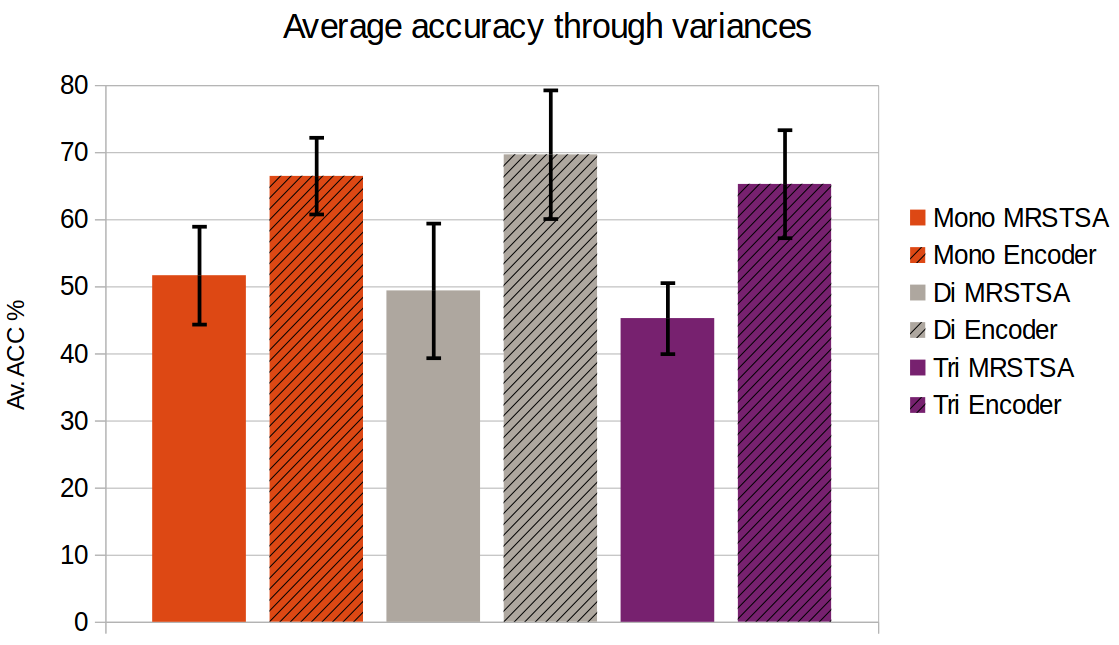
\includegraphics[width=0.6\textwidth]{AV_ACC.png}
    %\caption{Average classification accuracies across all variances for mono, di and trisyllabic words with Standard Error bars.
    %Mono means monosyllabic words, Di means disyllabic words and Tri means trisyllabic words.
    %Monosyllabic vocabulary: \textit{map, dog, mouse, with, truck.}
    %Disyllabic vocabulary: \textit{answer, doctor, teacher, summer, tennis.}  %and \textit{tennis}.
    %Trisyllabic vocabulary: \textit{computer, telephone, rectangle, tomato, magazine.} % and \textit{magazine}.
    %The white noise determines two levels of \gls{snr} average \gls{rms} power rate. One of 19.8 dB and the other of 13.8 dB.
    %The reverberation determines two levels of \gls{rt} value. One of 0.61 seconds while the other of 1.78 seconds.
    %Pitch variations determine a pitch move up from E to G and a pitch move down from E to C.}
    %\label{fig:AV_ACC}
%\end{figure}

%Since the \gls{el} has shown a prominent superiority respecting the \gls{mrstsa} in word classification performances, we produced a swept with \glspl{el} of different sizes in order to test if such improvement in the classification accuracy really comes from the intrinsic sequential characteristics in the algorithm or it is the result of a larger dimensionality present in the \gls{el}.

%In Table~\ref{EL_Swept} we show the initialization parameters for the different \glspl{el}.

%\begin{table}[h!]
%\centering
%\caption{\glspl{el} of different sizes in order to test how the number of \glspl{cc} affects the phonetic classification performance}
%\begin{tabular}{|l|l|l|l|l|}
%\hline
		%& Cortical Columns	& Number of Units	& Receptive Fields	& Cooley Nodes	\\ \hline
%Encoder Layer 0	& $1 * 1$		& $15 * 15$		& $1 * 1 (0)$		& 1		\\ \hline
%Encoder Layer 1	& $3 * 3$		& $15 * 15$		& $3 * 3 (1)$		& 1		\\ \hline
%Encoder Layer 2	& $9 * 9$		& $15 * 15$		& $9 * 9 (4)$		& 9		\\ \hline
%Encoder Layer 3	& $15 * 15$		& $15 * 15$		& $15 * 15 (7)$		& 25		\\ \hline
%Encoder Layer 4	& $21 * 21$		& $15 * 15$		& $15 * 15 (7)$		& 49		\\ \hline
%\end{tabular}
%\label{EL_Swept}
%\end{table}

%The \gls{el} 0 has one \gls{cc} with 15 for 15 (225) Neural Units, the \gls{el} 1 has 3 for 3 (9) \glspl{cc} with 225 Neural Units and so on. For each \gls{el} we used a number of Cooley computing nodes as to try to run 9 \glspl{cc} per Cooley Node distributed by means of \gls{omp} multi-threading operations. Fig.~\ref{fig:EL_Swept} shows the average phonetic word classification performance obtained for each \gls{el}. As can be seen in the figure, even though the \gls{el} 0 has less dimensions than the \gls{mrstsa} algorithm, \gls{el} 0 clearly outperforms such algorithm in the word classification task. This shows that the improvement in the performance has its root in the algorithmic sequential characteristics of the \glspl{el} and that this does not come exclusively from a larger dimensionality which would lead to a better discrimination.

%\begin{figure}[h!]
    %\centering
    %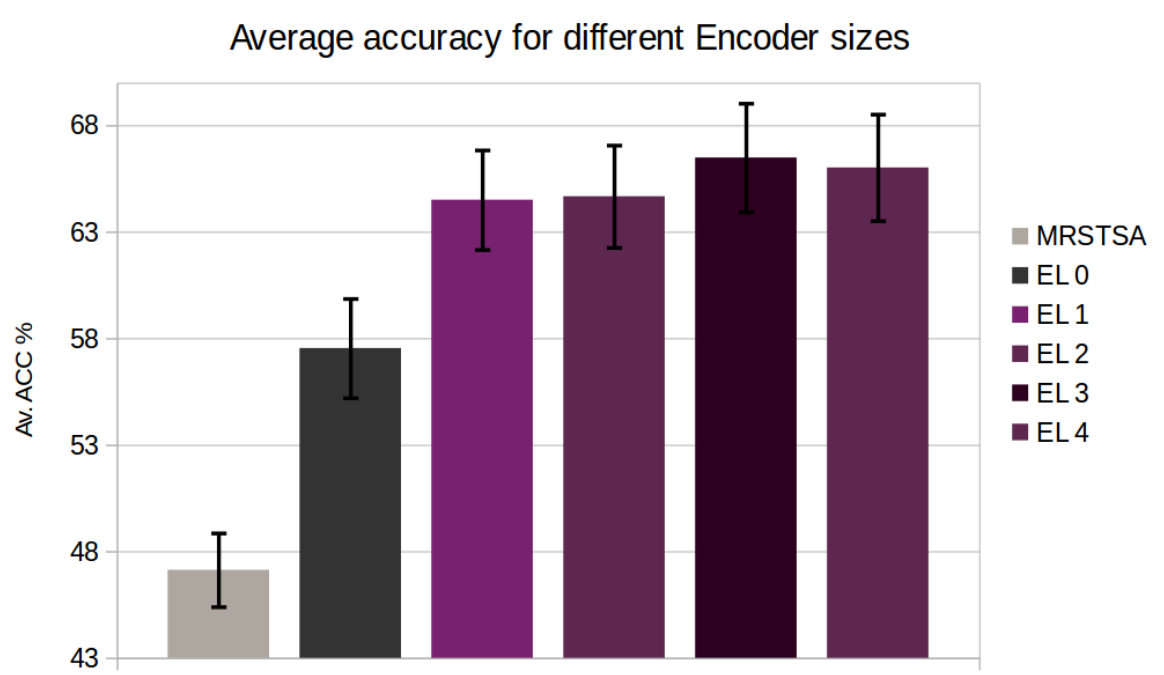
\includegraphics[width=0.6\textwidth]{EL_Swept.png}
    %\caption{Average classification performances tests with \glspl{el} of different sizes. The different \glspl{el} were trained with one corpus and tested with all corpora in the presence of the already used disturbances--such as white noise, reverberation and pitch variations. The bars show the total average for each \gls{el}. There is a sustained grow in the classification performance for \glspl{el} with more \glspl{cc}. Even though, the sharp jump in classification performance from the \gls{mrstsa} algorithm to the \gls{el} 0 shows that this improvement is originated in the algorithmic characteristics beyond a simple increment in the dimensionality of the representations.}
    %\label{fig:EL_Swept}
%\end{figure}

%Irrespective of the last asseveration, there is a clear tendency of the performance to grow with the size of the \gls{el}. Although the origin of such behavior comes from the greater dimensionality in larger \glspl{el} we also know that smaller \glspl{el} suffer from a distal dendrite sparsity problem which generates repetitive \glspl{mfe} and a lack of \glspl{sdr} whose origins are prediction faults produced in the processing of the stream of data.

%Although Fig.~\ref{fig:EL_Swept} shows the complete average in the performance for word classification tasks for each \gls{el}, the experimental procedure has an underlying complexity not shown by such figure. For each \gls{el} we got a different model trained with a different vocabulary. For example, we got three \glspl{el} 0, one trained using monosyllabic words, one trained using disyllabic words and one trained using trisyllabic words. Each of those \glspl{el} were tested using all the corpora, in this way we ended up having cross testing procedures in which an \gls{el} trained using monosyllabic words was tested not only using monosyllabic words but also di and trisyllabic words subjecting those \glspl{el} to the all kind of disturbances already mentioned--such as white noise, reverberation and pitch variations.

%Fig.~\ref{fig:EL_Cross_Performance} shows the average performances for all the \glspl{el}.

%\begin{figure}[h!]
    %\centering
    %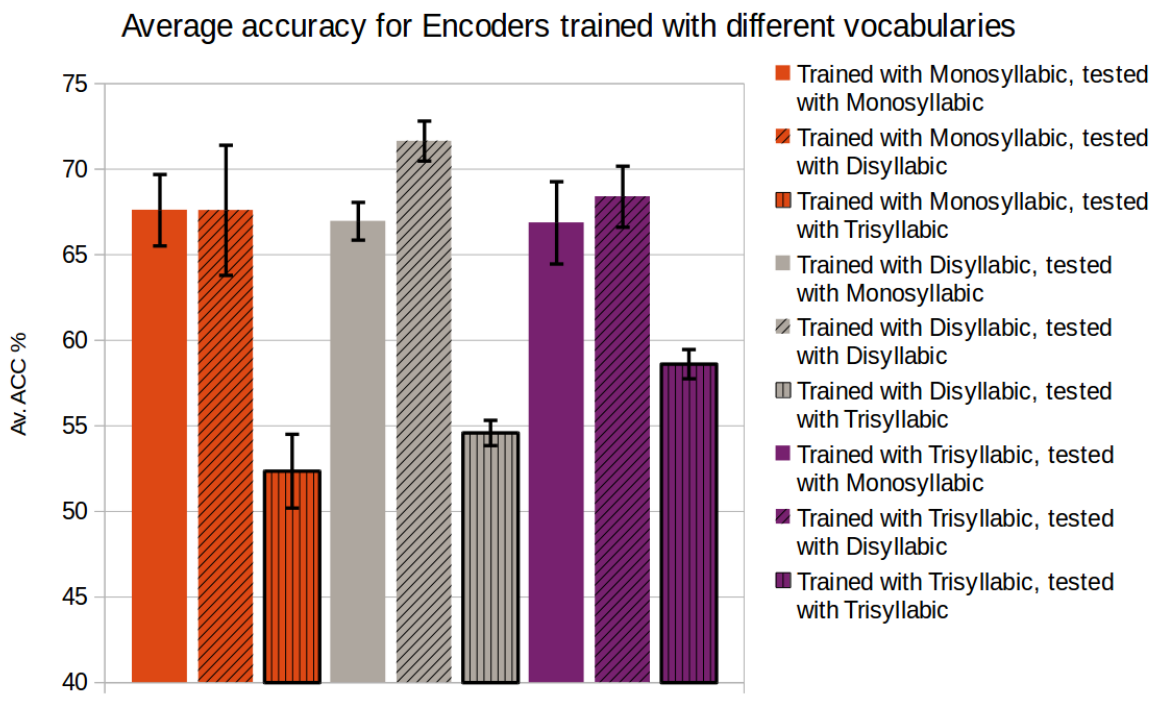
\includegraphics[width=0.6\textwidth]{EL_Cross_Performance.png}
    %\caption{Average classification performance tests with several \glspl{el} with different sizes. Each \gls{el} was trained using three different corpora--monosyllabic, disyllabic and trisyllabic words. Those \glspl{el} were tested using the three corpora. For example, an \gls{el} trained using monosyllabic words was tested using not only monosyllabic words but also di and trisyllabic words. This procedure was repeated for each \gls{el} listed in Table~\ref{EL_Swept} and all the \gls{el} performances were averaged to get the bars in this figure. This experimental procedure is similar to \emph{Self-taught Learning} implemented in~\cite{Raina:2007:SLT:1273496.1273592} in the sense that the data used to train the model was different from the labeled data used to test the phonetic features acquired by it. Orange bars show the performances of models trained with monosyllabic words, gray bars show the performances of models trained with disyllabic words and purple bars shows the performances of models trained with trisyllabic words. In the same fashion, solid bars show tests performed with monosyllabic words, diagonally striped bars show tests performed with disyllabic words while vertically striped bars show tests performed with trisyllabic words.}
    %\label{fig:EL_Cross_Performance}
%\end{figure}

%The \glspl{el} show to use the features acquired with one vocabulary in tests with other vocabularies. For example, looking at orange bars in Fig.~\ref{fig:EL_Cross_Performance} it is clear that \glspl{el} trained using monosyllabic words use its phonotactic features inferencing disyllabic words as well as monosyllabic words. The case depicted by purple bars shows that the phonotactic features acquired by models from certain vocabulary could get better performance inferencing other vocabularies deferent fron the one used to train the \glspl{el}. Respecting this last point we have to take into account that there is a clear decrease in performance for the classification of trisyllabic words respecting mono and disyllabic words. This decrease could be clearly originated in in a greater difficulty to classify larger words. Even though, if we pay attention only to vertically striped bars we will notice that the best performance is obtained when the words used to test the \glspl{el} is the same used to train it. A similar analysis could be done for solid and diagonally striped bars. Hence, there could be certain idiosyncratic behavior that shows better performance of the \glspl{el} for the words with which they were trained, as can be seen in the figure.














%these are the materials and methods used in the experimental procedures
\section{Materials and Methods}




\fi



\bibliographystyle{plain}
\bibliography{CARLA_Manuscript}

\end{document}
